\cotefile{5}
\scanpage{1}
IMAG

INSTITUT MONTPELLIERAIN

ALEXANDER GROTHENDIECK

\figure{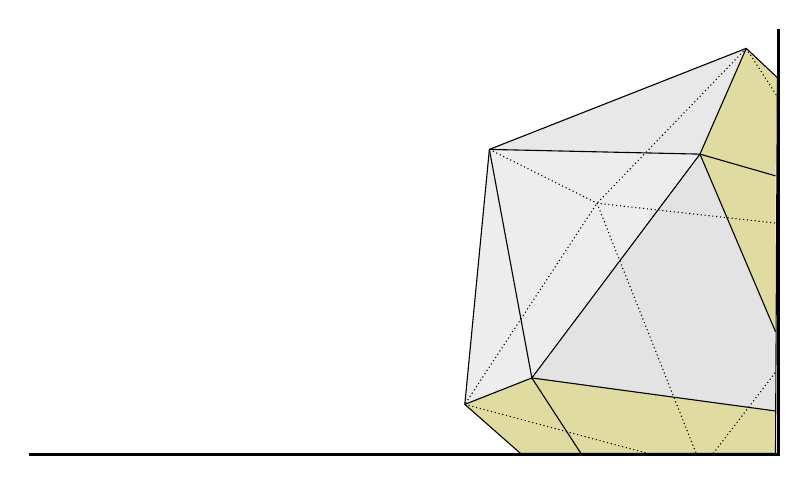
\begin{tikzpicture}[x=0.012cm,y=-0.012cm]
\fill[gray!18] (497,138)--(769,31)--(720,143)--cycle;
\fill[gray!14] (497,138)--(720,143)--(542,380)--(471,408)--cycle;
\fill[gray!22] (720,143)--(800,331)--(800,415)--(542,380)--cycle;
\fill[olive!28] (769,31)--(802,62)--(800,166)--(720,143)--cycle;
\fill[olive!28] (720,143)--(800,166)--(800,331)--cycle;
\fill[olive!28] (471,408)--(542,380)--(800,415)--(800,460)--(530,460)--cycle;
\draw (497,138)--(769,31)--(802,62)--(800,460)--(530,460)--(471,408)--cycle;
\draw (497,138)--(720,143)--(769,31);
\draw (720,143)--(800,166);
\draw (720,143)--(800,331);
\draw (497,138)--(542,380)--(720,143);
\draw (471,408)--(542,380)--(800,415);
\draw (542,380)--(594,460);
\draw[densely dotted] (497,138)--(611,195)--(800,216);
\draw[densely dotted] (769,31)--(611,195)--(471,408);
\draw[densely dotted] (611,195)--(716,460);
\draw[densely dotted] (471,408)--(665,460);
\draw[densely dotted] (734,460)--(800,374);
\draw[densely dotted] (769,31)--(802,82);
\draw[line width=1.3pt] (10,461)--(803,461)--(803,11);
\end{tikzpicture}}


\scanpage{3}
\diagram{\begin{tikzcd}[ampersand replacement=\&,column sep=large,row sep=large]
 \& X_{zar}\arrow[dl]\arrow[dr] \& \\
X_{conn}\arrow[rr,dashed]\arrow[dr,"\text{équiv -- car 0}"]\arrow[dd,"\substack{\text{équiv.}\\\text{si }X/S\text{ lisse}}"'] \& \& X_{\mathbb{P}\text{-}conn.}\arrow[dl,dashed]\arrow[dd,"\substack{\text{équiv}\\\text{si }X/S\text{ lisse}}"]\\
 \& X_{strat}\arrow[dd] \& \\
X_{cris}\arrow[rr,dashed]\arrow[dr]\arrow[dddr] \& \& X_{\mathbb{P}\text{-}cris}\arrow[dl,dashed]\arrow[dddl]\\
 \& X_{inf}\arrow[dd] \& \\
 \& \& \\
 \& X_{zar} \&
\end{tikzcd}}

\margin{$\left.\vphantom{\begin{matrix}X\\X\\X\\X\end{matrix}}\right\}$ morphismes de topos \uline{annelés}
[$\dashrightarrow$ définis si $X$ de torsion sur $\mathbb{Z}$]}

\margin{NB $\mid$ $S$ sous-entendu dans notations.}

Les flèches à valeurs dans $X_{zar}$ donnent lieu à des \uline{isomorphismes de localisation} \uline{\unsure{gerbienne|galoisienne}}, resp. des suites spectrales \unsure{intéressantes} --

\margin{détermination des \uline{points} de ces topos ?}

Les flèches en provenance de $X_{zar}$ donnent lieu à une suite exacte
\[
0\longrightarrow J\longrightarrow\mathcal{O}_{X}\longrightarrow\mathcal{O}_{X_0}\longrightarrow0
\]
\margin{\figure{\begin{tikzpicture}\draw (0,-1.1)--(.65,1.1);\node[anchor=west,text width=4cm] at (.6,0) {dire que $\operatorname{Mod}(X_{zar})\xrightarrow{\approx}\operatorname{Mod}(\mathcal{O}_{X_0})$};\end{tikzpicture}}}

Pour un module inversible $\underline{L}$ sur $X_{zar}$, \unsure{on|--} définit une classe de Chern $c^{\unsure{1|'}}(\underline{L})$ dans $H^2(X_{cris})$ et $H^2(X_{\mathbb{P}\text{-}cris})$, qui sont compatibles si $X$ de torsion. Sur $X_{cris}$, son annulation est NS pour que $\underline{L}$ provienne d'un Module inversible sur $X_{cris}$ [donc dans le cas relatif lisse \deleted{\unsure{disons}} qu'il admette une connexion intégrable].
\mspage{2}


\scanpage{4}
-32-

In view of th.11, it is natural to define a homomorphism
\[
\rho_\infty:I_K\longrightarrow F_\infty^*=(R\otimes F)^*
\]
by putting $\rho_\infty(a)=\varepsilon(a)\psi_\infty(a_\infty^{-1})$, where $a_\infty$ is the infinite component of the idèle $a$. This homomorphism is obviously characterized by the fact that it is continuous, trivial on $K^*$, and coincides with $\varepsilon$ on the group $I_K^\infty$ of idèles whose infinite component is 1.

Let $\sigma:F\to C$ be a homomorphism. The composition
\[
\chi_\sigma:I_K\xrightarrow{\rho_\infty}(R\otimes F)^*\xrightarrow{1\otimes\sigma}C^*
\]
is continuous and trivial on $K^*$ ; that is, $\chi_\sigma$ is a ``Grössencharakter'' in the broad sense (having values in $C^*$ rather than in the unit circle); it is essentially the same as the Grössencharakter defined in [18], p.148. For each valuation $v$ of $K$, the restriction of $\chi_\sigma$ to $U_v(K)$ is $\sigma\circ\varphi_v$, and, since $\sigma$ is injective, it follows that \uline{the exponent at} $v$ \uline{of the conductor of} $\chi_\sigma$ \uline{is equal to the number} $n_v$ \uline{of th.}6. Hence :

THEOREM 12 - \uline{The conductor of the abelian variety} $A$ \uline{is the} $2d$-th \uline{power of the conductor of} $\chi_\sigma$ ; \uline{in particular}, \uline{the support of the conductor of} $\chi_\sigma$ \uline{is the set of valuations of} $K$ \uline{where} $A$ \uline{has bad reduction}.

For elliptic curves, the second statement was proved by Deuring [7].
\mspage{3}


\scanpage{5}
$W$ vecteurs de Witt sur corps parfait $k$.

$\nu\geq1$ entier.

On s'intéresse à la catégorie des \deleted{algèbres} \inserted{anneaux} artiniens \deleted{\unsure{sur} algèbres sur} \inserted{de corps rés.} $k$ à idéal maximal muni de puiss. divisées $\nu$-nilpotentes. On va construire un objet initial de cette catégorie.

Pour ceci, on note que les $\Lambda$ sont des algèbres sur $W$ (\unsure{Cohen}). et que l'élément $\lambda_0=p\in W$ s'envoie dans $\unsure{\mathfrak{m}_{\Lambda}|\mathfrak{m}\Lambda}$. Donc $\Lambda$ reçoit
\[
\begin{split}
W^{(\nu)}=W[\Lambda_0,\ldots,\Lambda_\nu]/(&\Lambda_0^p-p!\Lambda_1,\Lambda_1^p-\frac{p^2!}{(p!)^p}\Lambda_2,\ldots,\Lambda_{\nu-1}^p-\frac{p^\nu!}{(p^{\nu-1}!)^p}\Lambda_\nu,\Lambda_\nu^p;\\
&\Lambda_0-\deleted{\unsure{p}}\lambda_0)
\end{split}
\]
[\deleted{\unsure{anneau avec idt}} \inserted{$W$-algèbre} avec idéal $J=(\Lambda_0,\ldots\Lambda_\nu)$ à puiss. div. $\nu$-nilpotentes, \uline{universel} pour les algèbres sur $W$, avec idéal à puissances divisées $\nu$-nilpotentes contenant l'image de $\lambda_0$]. NB. $\Lambda_\nu=\gamma^{p^\nu}(\Lambda_0)$; on utilise le fait que dans $W$ les nbs. premiers $l\ne p$ sont inversibles.

On \deleted{$\unsure{W^{(\nu)}}$} on voit de suite que $W^{(\nu)}$ est artinien de corps résiduel $k$, \deleted{(\unsure{c'est un vrai anneau de} \unsure{mettre|enlever} la relation $\Lambda_0-\lambda_0$), \unsure{qui}} \inserted{l'idéal maximal étant précisément $J$}

On va calculer explicitement $W^{(\nu)}$. Pour ceci, \deleted{\unsure{on pose}} on commence par l'anneau plus simple
\[
\deleted{\unsure{W}}\quad A^{(\nu)}=W[\Lambda_0,\ldots\Lambda_\nu]/(\Lambda_0^p-p!\Lambda_1,\ldots,\Lambda_\nu^p)
\]
(on omet la relation $\Lambda_0-\lambda_0$). On pose aussi
\[
\lambda_r=\frac{p^{p^r}}{p^r!}=\gamma^{p^r}_{\text{habituel}}(p)
\]
et on pose
\[
\Lambda_i=\lambda_i+\Theta_i\qquad 0\leq i\leq\nu.
\]
Par abus de \unsure{langage}, on désignera par la suite par $\Lambda_i$, $\Theta_i$ les images de $\Lambda_i$, $\Theta_i$ dans $A^{(\nu)}$. Alors $A^{(\nu)}$ \unsure{est} une
\mspage{4}


\scanpage{6}
base sur $W$ formée des
\[
\Theta_0^{a_0}\cdots\Theta_\nu^{a_\nu}\qquad 0\leq a_i\leq p-1\quad\text{pour }i=0,\ldots,\nu.
\]
Il faut maintenant diviser par l'idéal \inserted{$I$} engendré par $\Theta_0$. On a le

\uline{Lemme} Pour que $\displaystyle\sum_{\substack{a=(a_0,\ldots a_\nu)\\0\leq a_i\leq p-1}}w_a.\Theta_0^{a_0}\cdots\Theta_\nu^{a_\nu}$ soit dans l'idéal engendré par $\Theta_0$, il faut et il suffit que

a) pour $\forall\ a=(a_0,\ldots a_\nu)$, si \inserted{$a\ne0$ et si} $a_i$ est la première composante non nulle de $a$, on ait $\deleted{\unsure{p}}w_a\in p^iW$

b) le coefficient $w_0$ de $1$ soit dans $p^{c(\nu)}W$, où
\[
c(\nu)=\nu+p[p^\nu-(p^{\nu-1}+p^{\nu-2}+\cdots+1)]
\]

\uline{Dém.} \uline{Condition suffisante} Résulte des relations
\[
\left\{\begin{aligned}p^i\Theta_i&\in I\\p^{c(\nu)}&\in I\end{aligned}\right.
\]
La première relation par récurrence sur $i\geq0$. Si $i=0$ c'est $\Theta_0\in I$, \deleted{\unsure{c'est le}} trivial. Supposons qu'on sache $p^i\Theta_i\in I$ $(i\leq\nu-1)$ on utilise
\[
(\Theta_i+\lambda_i)^p=\frac{p^{i+1}!}{(p^i!)^p}(\Theta_{i+1}+\lambda_{i+1}),
\]
qui s'écrit
\[
\deleted{\unsure{\Theta_i^p=}}\quad\sum_{\alpha=1}^{\unsure{p-1|p}}\inserted{C_i^p}\Theta_i^\alpha\lambda_i^{p-\alpha}
=\left(\deleted{-\lambda_i^p}+\deleted{\frac{p^{i+1}!}{(p^i!)^p}\unsure{\lambda_{i+1}|\Theta_{i+1}}}+\frac{p^{i+1}!}{(p^i!)^p}\Theta_{i+1}\right)
\]
multipliant par $p^i$, on trouve que, compte tenu que $p^i\Theta_i\in I$ donc $p_i\Theta_i^\alpha=0$ si $\alpha\geq1$ :
\[
p^i\frac{p^{i+1}!}{(p^i!)^p}\Theta_{i+1}=0
\]
Or on constate que
\[
v_p\left(\frac{p^{i+1}!}{(p^i!)^p}\right)=1
\]
\mspage{5}


\scanpage{7}
donc la relation précédente équivaut à
\[
p^{i+1}\Theta_{i+1}=0
\]
On a donc prouvé les relations $p^i\Theta_i=0$. Pour la deuxième relation, on écrit
\[
(\lambda_\nu+\Theta_\nu)^p=0\qquad\text{i.e.}
\]
\[
\lambda_\nu^p+\sum_{i=1}^p C_i^p\Theta_\nu^i\lambda_\nu^{p-i}=0
\]
Multiplions par $p^\nu$ et utilisons que $p^\nu\Theta_\nu\in I$ donc $p^\nu\Theta_\nu^\alpha\in I$ si $\alpha\geq1$, on trouve
\[
p^\nu\lambda_\nu^p\in I
\]
Or on a
\[
v_p(p^\nu\lambda_\nu^p)=\nu+p\,v_p\left(\underbrace{\lambda_\nu}_{\inserted{=\frac{p^{p^\nu}}{p^\nu!}}}\right)=\nu+p\left(p^\nu-\frac{p^\nu-1}{p-1}\right)=c(\nu)
\]
Pour prouver que la condition est nécessaire, il suffit de noter que l'ensemble $I'$ formé des éléments satisfaisant les cond. \deleted{\unsure{de}} ci-dessus données (qui satisfait $I'\subset I$, $\Theta_0\in I'$) est bien un \uline{idéal}, i.e. \deleted{est stable} (comme c'est un sous-$W$-module) est stable par multiplication par $\Theta_0,\ldots,\Theta_\nu$. La vérification est facile et laissée au lecteur.

\margin{!}

\uline{Corollaire} Soit, pour tt $i$, $E_i$ un syst. de représentants de $W/p^iW$. Alors un élément de $W^{(\nu)}$ s'écrit de façon unique sous la forme
\[
\sum w_{a_1,\ldots,a_\nu}\dot{\Theta}_1^{a_1}\cdots\dot{\Theta}_\nu^{a_\nu}
\]
avec
\[
\left\{\begin{aligned}
&0\leq a_i\leq p-1\qquad(1\leq i\leq\nu)\\
&w_{a_1,\ldots,a_\nu}\in E_i\quad\text{si }a_i\text{ est la première coordonnée non nulle de }(a_1,\ldots,a_\nu).
\end{aligned}\right.
\]
\mspage{6}


\scanpage{8}
\[
\left\{\ w_0\in E_{c(\nu)}\right.
\]

\uline{Lemme} Soit $1\leq r\leq\nu$, et soit $W^{(\nu,r)}$ le quotient de $W^{(\nu)}$ par l'idéal engendré par $\dot{\Theta}_1,\ldots,\dot{\Theta}_r$. \deleted{Alors le} Soit $\deleted{\unsure{A}}\ I_{\nu,r}$ l'idéal de $A^{(\nu)}$ engendré par $\Theta_0,\ldots,\Theta_r$, de sorte que $A^{(\nu)}/I_{\nu,r}\simeq W^{(\nu,r)}$\figure{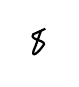
\begin{tikzpicture}[x=.14cm,y=.14cm]\draw[thick] (.8,2)--(-.3,1.5) .. controls (-.7,.9) and (1.2,1) .. (.55,.4) .. controls (-.1,-.5) and (-.6,-.6) .. (-.1,.4)--(.4,1.8);\end{tikzpicture}}. Pour que $\sum w_a\Theta_0^{a_0}\cdots\Theta_\nu^{a_\nu}$ soit dans $I_{\nu,r}$, il f. et s. que

a) pour tt \deleted{$\alpha,\ 1\leq\alpha\leq\nu-r$, \unsure{pour un}} \inserted{$a=(a_0,\ldots a_\nu)\ne0$,} \deleted{\unsure{si}} si $a_i$ est la première composante non nulle et si $i>r$, on ait $\deleted{\unsure{p}}$
\[
w_a\in p^{i-r}W
\]
b) On ait
\[
w_0\in p^{c(\nu)-r}W
\]

\uline{Cor.} Forme normale d'un élément de $W^{(\nu,r)}$ :
\[
\sum w_{a_{r+1},\ldots,a_\nu}\Theta_{r+1}^{a_{r+1}}\cdots\Theta_\nu^{a_\nu}
\]
avec
\[
\left\{\begin{aligned}
&w_{a_{r+1},\ldots a_\nu}\in E_i\deleted{\unsure{-r}}\quad\text{si }a_{r+i}\text{ est le premier des }a_\alpha\text{ qui est }\ne0\\
&w_0\in E_{c(\nu)-r}
\end{aligned}\right.
\]
\mspage{7}


\scanpage{9}
$W$ vecteurs de Witt

$\Lambda_0\cdots\Lambda_\nu$ indéterminées, \unsure{liées|liés} par
\[
\left\{\begin{aligned}
\Lambda_i^p&=\frac{p^{i+1}!}{(p^i!)^p}\Lambda_{i+1}\qquad\text{si }0\leq i\leq\nu-1\\
\Lambda_\nu^p&=0
\end{aligned}\right.
\]
Ceci implique
\[
\Lambda_0^{a_0}\cdots\Lambda_\nu^{a_\nu}=0\quad\text{si }\sum a_ip^i\geq p^{\nu+1}\qquad(a_i\geq0
\]
\deleted{\unsure{Comme}} \uline{Dém} \figure{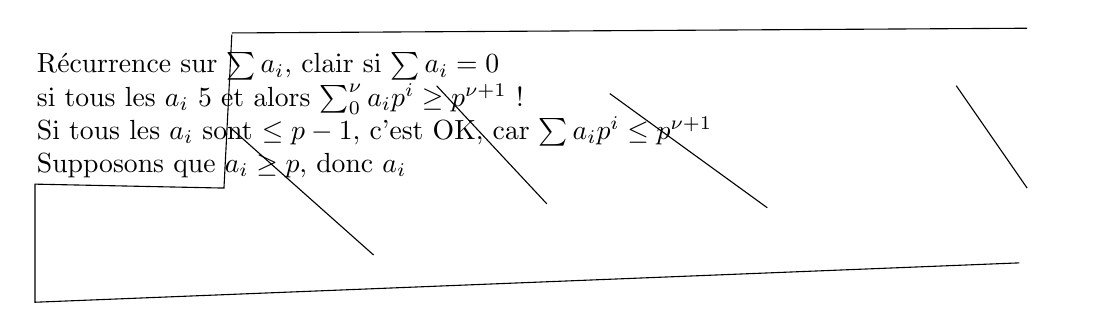
\begin{tikzpicture}[x=1cm,y=1cm]
\node[anchor=north west,text width=13cm,align=left] at (0,0) {\deleted{Récurrence sur $\sum a_i$, clair si $\sum a_i=0$\par si tous les $a_i$ \illegible{5} et alors $\sum_0^\nu a_ip^i\geq p^{\nu+1}$ !\par Si tous les $a_i$ sont $\leq p-1$, c'est OK, car $\sum a_ip^i\leq p^{\nu+1}$\par Supposons que $a_i\geq p$, \unsure{donc} $a_i$}};
\draw (2.6,.12)--(12.7,.18);
\draw (2.6,.1)--(2.5,-1.85)--(.1,-1.8)--(.1,-3.3)--(12.6,-2.8);
\draw (2.6,-1.1)--(4.4,-2.7);
\draw (5.2,-.55)--(6.6,-2.05);
\draw (7.4,-.65)--(9.4,-2.1);
\draw (11.8,-.55)--(12.7,-1.85);
\end{tikzpicture}}

\deleted{\unsure{si}} \deleted{\unsure{est}}

\uline{Lemme}
\[
\Lambda_0^{a_0}\Lambda_1^{a_1}\cdots\Lambda_\nu^{a_\nu}=c\Lambda_0^{b_0}\cdots\Lambda_{\nu-1}^{b_{\nu-1}}\Lambda_\nu^{b_\nu},\qquad c\in W
\]
avec $0\leq b_\alpha\leq p-1$ pour $0\leq i\leq\uline{\nu-1}$ et $b_\nu$ a priori \unsure{qq.}, et
\[
\sum_0^\nu a_ip^i=\sum_0^\nu b_ip^i
\]
Pour le voir, on \deleted{procède} par récurrence, \deleted{\unsure{sur} $\sum a_i$, \unsure{de sorte}} \inserted{transformons} l'expression en une expression $c\Lambda_0^{a'_0}\cdots\Lambda_\nu^{a'_\nu}$, avec les $a'_\alpha\leq p-1$.
\deleted{\unsure{par} $\sum a_i$, \unsure{puis tous} $a_i$ \unsure{tels}} \inserted{\unsure{le premier des} $a'_\alpha\leq p-1$}
\deleted{Donc \unsure{pour} $\sum a_i$, \unsure{si on a}} \inserted{$\alpha\leq p-1\ (i\leq\nu-1)$}
Si \unsure{nous} (pour $a_i$ \deleted{$\unsure{(i\leq\nu-1)}$} est $\geq p$, on écrit $a_i=pq_i+a'_i$, d'où
\[
\Lambda_i^{a_i}=(\Lambda_i^p)^{a'_i}\Lambda_i^{\alpha_i}=(c_i\Lambda_{i+1})^{a'_i}\Lambda_i^{\alpha_i}=c'\Lambda_{i+1}^{a'_i}\Lambda_i^{\alpha_i}
\]
donc
\[
\Lambda_0^{a_0}\cdots\Lambda_\nu^{a_\nu}=c\Lambda_0^{a_0}\cdots\Lambda_i^{a'_i}\Lambda_{i+1}^{\overbrace{a_{i+1}+q_i}^{\inserted{a'_{i+1}}}}\Lambda_{i+2}^{a_{i+2}}\cdots,
\]
et évidemment on a
\[
\sum a_ip^i=\sum a'_ip^i,
\]
car
\[
\deleted{a'_ip^i+}\quad\underline{a'_ip^i+\underline{(a_{i+1}+q_i)}}p^{i+1}=\underbrace{(a'_i+q_ip)}_{a_i}p^i+a_{i+1}p^{i+1}.
\]
Or, si on a $\sum b_ip^i\geq p^{\nu+1}$, alors \deleted{\unsure{on}} (et alors seulement) \deleted{$\unsure{p}$} $b_\nu\geq p$, donc $\Lambda_\nu^{b_\nu}$ est un \deleted{\unsure{multiple de} $\unsure{\Lambda_\nu^p}$} multiple de $\Lambda_\nu^p$, or $\Lambda_\nu^p=0$. OK.
\mspage{8}


\scanpage{10}
\mspage{\unsure{9|6}}
\mspage{34}
\[
(D-\operatorname{div}(g)).(w_1\times\cdots\times A\times\cdots\times w_5)=0.
\]
($h$-ième facteur égal à $A$ dans la seconde parenthèse). Supposons le diviseur $D-\operatorname{div}(g)$ non nul, et soit $Z$ l'une de ses composantes. D'après la relation précédente, $Z$ se projette suivant une sous-variété de codimension $\geq2$ sur chacun des produits partiels formés avec quatre des facteurs du produit $B=A\times A\times A\times A\times A$. Ceci est impossible, puisque $Z$ est de codimension $1$ relativement à $B$. On a bien $D=\operatorname{div}(g)$.

Soit maintenant $z$ un point générique de $A$ sur le corps $K(a_0,a_1,a_2,b_0)$, et considérons la fonction $g'$ sur $A$, définie sur $K$, telle qu'on ait
\[
g'(z)=g(a_0,a_1,a_2,b_0,z).
\]
D'après ([14], IX, 2, th.3), on a
\[
a_0\times a_1\times a_2\times b_0\times\operatorname{div}(g')=\operatorname{div}(g).(a_0\times a_1\times a_2\times b_0\times A).
\]
Or, d'après l'expression de $\operatorname{div}(g)$ obtenue plus haut, et d'après le lemme 2, on a
\[
\operatorname{div}(g).(a_0\times a_1\times a_2\times b_0\times A)=a_0\times a_1\times a_2\times b_0\times X_{\underline{a}}.
\]
On a donc
\[
\operatorname{div}(g')=X_{\underline{a}}.
\]
De plus, le point $c$, ainsi que le point $c_0=a_0\times a_1\times a_2\times b_0\times b_0$, n'appartiennent pas au support de $\operatorname{div}(g)$. La fonction $g$ est donc définie en $c$ et en $c_0$, et on a les relations
\[
g(c)=g'(b_1)\qquad g(c_0)=g'(b_0).
\]
Remarquons en outre que, si $\bar{y}_1$ est un point générique de $A$ sur $K(x_0,x_1,x_2,y_0,y_1)$, on a
\[
g(x_0,x_1,x_2,y_1,\bar{y}_1)=g(x_0,x_1,x_2,y_0,\bar{y}_1)\,g(x_0,x_1,x_2,y_0,y_1)^{-1}.
\]


\scanpage{11}
\[
\begin{aligned}
\overset{\deleted{\unsure{\mu+1}}}{v_p}(n!)={}&a_\nu v_p(p^\nu!)+\cdots+a_{\mu+1}v_p(p^{\mu+1}!)\\
&-v_p(p^{\mu+1}!)+\underbrace{(\mu+1)+(p-1)[v_p(p^\mu!)+\cdots+v_p(p)]}_{\deleted{\unsure{p^{\mu+1}}}}
\end{aligned}
\]
\[
v_p(1)=0
\]
\[
v_p(p)=1+(p-1).0=1
\]
\[
v_p(p^2)=2+(p-1)1=p+1
\]
\[
v_p(p^3)=3+\inserted{(p-1)}((p+1)+1)=p^2+p+1
\]
\[
\begin{aligned}
v_p(p^4)&=4+(p-1)[p^2+2p+3]\\
&=4+p^3+2p^2+3p\\
&\phantom{={}}\quad-p^2-2p-3\qquad=\deleted{4+}p^3+p^2+p+1
\end{aligned}
\]
\[
v_p(p^\nu)=p^{\nu-1}+p^{\nu-2}+\cdots+\deleted{\unsure{p}}1=\frac{p^\nu-1}{p-1}
\]
\[
\begin{aligned}
v_p(p^{\nu+1})&=\nu+1+(p-1)[p^{\nu-1}+2p^{\nu-2}+3p^{\nu-3}\cdots+\nu p^0]\\
&=\nu+1+p^\nu+2p^{\nu-1}+3p^{\nu-2}\cdots+\nu p\\
&\phantom{={}}\quad-p^{\nu-1}-2p^{\nu-2}-\cdots-(\nu-1)p-\nu\\
&=p^\nu+p^{\nu-1}+\cdots+p+1
\end{aligned}
\]
\[
\sum a_\nu(p^{\nu-1}+p^{\nu-2}\cdots+1)
\]
\[
\begin{aligned}
v_p(n!)(p-1)&=a_1(p-1)+a_2(p^2-1)+\cdots+a_\nu(p^\nu-1)\\
&=n-a_0-a_1-\cdots-a_\nu\\
&=
\end{aligned}
\]
\[
\boxed{a_1+a_2(p+1)+a_3(p^2+p+1)+a_4(p^3+p^2+p+1)+\cdots}
\]
\[
a_1+pa_2\deleted{\unsure{\longrightarrow}}+p^2a_3\qquad p
\]
\figure{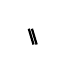
\begin{tikzpicture}[x=.2cm,y=.2cm]\draw[thick] (0,1)--(.3,0);\draw[thick] (.2,1)--(.5,0);\end{tikzpicture}}
\[
\boxed{\boxed{v_p(n!)=\frac{n-\sum a_i}{(p-1)}}}
\]
\mspage{10}


\scanpage{12}
45bis

\margin{\textcircled{x}}
(v)- Supposons $\underline{a}$ rationnel sur $K$, et $\underline{q}$ définie sur $K$. Alors $\xi_0(\underline{q}_{\underline{a}_m})$ est définie sur $K$ pour tout $m$. Soit $x$ un point de $A$, rationnel sur une extension algébrique de degré fini $L$ de $K$. Pour $\underline{q}$, $\underline{a}$, $x$ et $m$ fixés, le nombre $(\xi_0(\underline{q}_{\underline{a}_m}))((x)-(0),v)$ ne dépend que de la valeur absolue $w$ induite par $v$ sur $L$. \margin{\figure{\begin{tikzpicture}\draw[thick] (0,0)--(.03,-.35);\end{tikzpicture}}}Par passage à \deleted{\unsure{l'infini}} la limite pour $m$ infini, on en déduit qu'il en est de même de $(\mu(\underline{q},\underline{a}))((x)-(0),v)$, autrement dit que $\mu(\underline{q},\underline{a})$ est définie sur $K$.
\margin{$\longrightarrow$ \textcircled{xx} p.45}
\mspage{11}


\scanpage{13}
\[
v_p\left(\frac{\pi^n}{n!}\right)\ge0\quad\inserted{\text{\unsure{resp. }} >0}\qquad\text{pour \unsure{tout} }n\ ?
\]
\[
v_p\left(\frac{\pi^n}{n!}\right)\longrightarrow+\infty\qquad\text{pour }n\longrightarrow+\infty
\]
\[
\deleted{\unsure{(p-1)}}\quad v_p\left(\frac{\pi^n}{n!}\right)=\deleted{\unsure{(p-1)}}n v_p(\pi)-\frac{\{n-\operatorname{chif}(n)\}}{p-1}\ge0
\]
\[
\Updownarrow\qquad v_p(\pi)\ge\frac{1-\dfrac{\operatorname{chif}(n)}{n}}{p-1}
\]
\[
\deleted{v_p(\pi)}\qquad\operatorname{chif}(n)/n\longrightarrow0
\]
\deleted{$\dfrac{\operatorname{chif}(n)}{n}$ \unsure{fonction décroissante de $n$, tjs $\le1$}}
\[
\operatorname{chif}(n)\le1
\]
\[\unsure{c}\]
\margin{$\unsure{\frac q6|\ne}$}
\[
\begin{aligned}
n&=a_0+a_1p+\cdots+a_\nu p^\nu\\
\operatorname{chiff}(n)&=a_0+a_1+\cdots+a_\nu
\end{aligned}
\]
si $a_\nu\ne0$, on \unsure{trouve|a}
\[
\begin{aligned}
\operatorname{chiff}n&\le(p-1)\nu\deleted{\unsure{+1}}\\
n&\ge p^\nu\\
\frac{\operatorname{chiff}n}{n}&\le\frac{(p-1)\nu}{p^\nu}\longrightarrow0
\end{aligned}
\]
donc
\figure{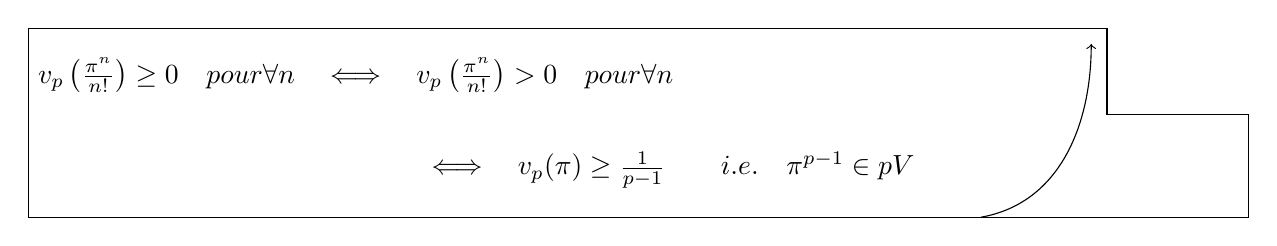
\begin{tikzpicture}
\node[anchor=west] at (0,1.2) {$v_p\left(\frac{\pi^n}{n!}\right)\ge0\quad\text{pour }\forall n\quad\Longleftrightarrow\quad v_p\left(\frac{\pi^n}{n!}\right)>0\quad\text{pour }\forall n$};
\node[anchor=west] at (5,0) {$\Longleftrightarrow\quad v_p(\pi)\ge\frac1{p-1}\qquad\text{i.e.}\quad\pi^{p-1}\in pV$};
\draw (0,1.8)--(13.7,1.8)--(13.7,0.7)--(15.5,0.7)--(15.5,-0.6)--(0,-0.6)--cycle;
\draw[->] (12.1,-0.6) to[out=10,in=-90] (13.5,1.6);
\end{tikzpicture}}
\[
(p-1)v_p\left(\frac{\pi^n}{n!}\right)=n[(p-1)v_p(\pi)-1]+\operatorname{chif}(n)
\]
Si $v_p(\pi)=\dfrac1{p-1}$, c'est $\operatorname{chif}(n)$, qui ne tend pas vers $+\infty$

Si $v_p(\pi)>\dfrac1{p-1}$, on \unsure{trouve} $\underbrace{\alpha n+\operatorname{chif}(n)}_{\displaystyle =n\left(\alpha+\frac{\operatorname{chif}(n)}n\right)\sim\alpha n}$, \inserted{$\alpha>0$,} (qui tend vers $\infty$

Donc \deleted{\unsure{condition}}
\[
\boxed{v_p\left(\frac{\pi^n}{n!}\right)\longrightarrow+\infty\quad\Longleftrightarrow\quad v_p(\pi)>\frac1{p-1}}
\qquad\boxed{\begin{gathered}\text{i.e. }p=\operatorname{unit}\pi^r,\\\text{avec }r<p-1\end{gathered}}
\]
\mspage{12}


\scanpage{14}
\figure{\begin{tikzpicture}[x=.009cm,y=-.009cm,every node/.style={anchor=west}]
\node at (0,0) {p.64}; \node at (140,0) {l.28}; \node at (380,0) {13)).};
\node at (150,60) {l.42}; \node at (370,60) {[5]};
\node at (0,140) {p.66}; \node at (180,140) {l.44,49}; \node at (450,140) {$\sigma$};
\node at (0,220) {p.67}; \node at (180,220) {l.26}; \node at (400,220) {Si}; \node[draw,ellipse] at (590,220) {minuscule};
\node at (180,280) {l.30}; \node at (420,280) {id};
\node at (180,340) {l.30}; \node at (420,340) {$\overline S=\operatorname{Spec}(\overline k)$.};
\node at (180,410) {l.33}; \node at (420,410) {noethérien\textcircled{s}.};
\node at (180,465) {l.48}; \node at (410,465) {\unsure{encore, encore}};
\node at (0,545) {p.68}; \node at (180,545) {l.57}; \node at (410,545) {1)). Alors};
\node at (930,545) {(\uuline{double parenthèse}, point)};
\node at (190,605) {l.61}; \node at (400,605) {$\sigma$};
\node at (0,670) {p.69}; \node at (190,670) {l.50}; \node at (410,670) {7.9.4),};
\node at (0,760) {p.70}; \node at (190,760) {l.21}; \node at (480,760) {\uline{Suppr. virgule} !!!};
\node at (0,840) {p.71}; \node at (190,840) {l.14}; \node at (430,840) {le composé};
\node at (0,925) {p.\deleted{74}\textcolor{red}{\inserted{73}}}; \node at (190,925) {l.62}; \node at (430,925) {le composé};
\node at (0,1010) {p.75}; \node at (190,980) {l.52}; \node at (430,980) {$X_K$}; \node[draw,ellipse] at (870,955) {$K$ maj.};
\node at (0,1090) {p.76}; \node at (250,1080) {l.61}; \node at (490,1080) {Compléter \unsure{bibliographie|bibliogr.} par [6]};
\draw[red,line width=1pt] (-8,-8)--(-10,8) (130,-8)--(125,8) (145,45)--(140,65) (-5,125)--(-10,148) (160,130)--(155,153) (0,205)--(-5,230) (170,205)--(165,230) (175,266)--(172,289) (175,328)--(172,349) (175,398)--(172,418) (175,450)--(172,475) (-5,535)--(-10,555) (175,535)--(170,555) (195,590)--(190,615) (-10,653)--(-15,678) (190,655)--(185,678) (-15,747)--(-20,772) (205,745)--(200,770) (-15,827)--(-20,850) (185,825)--(180,850) (-20,913)--(-25,938) (190,910)--(185,935) (-15,997)--(-20,1020) (195,970)--(190,990) (-20,1075)--(-25,1100) (250,1065)--(245,1085);
\draw[line width=.7pt] (350,300)--(1160,1120) (60,655)--(540,1120)--(520,1080) (860,200) to[out=-25,in=135] (1400,680);
\end{tikzpicture}}
\mspage{13}


\scanpage{15}
\margin{\unsure{Frobeniuseries|Frobeniuscria}}
\mspage{14}


\scanpage{16}
\unsure{General non-sens} sur Frobenius

1) Soit
\diagram{\begin{tikzcd}[ampersand replacement=\&]
X\arrow[r,"f_X"]\arrow[d,"g"']\&X\arrow[d,"g"]\\
Y\arrow[r,"f_Y"']\&Y
\end{tikzcd}}
un diagramme commutatif, à isom donné près, de topos. Si $E$ est un \deleted{complexe de} faisceaux \deleted{abéliens} \inserted{d'ens} sur $X$, on a \deleted{(sous des conditions, en degré \unsure{convenable})} un hom de changement de base
\[
\text{(1.1)}\qquad c_E:f_Y^*(g_*(E))\longrightarrow g_*(f_X^*(E))
\]
Si donc on a encore un hom
\[
\text{(1.2)}\qquad F_E:f_X^*(E)\unsure{-|\longrightarrow}E
\]
on en déduit
\[
g_*(F_E):g_*f_X^*E\unsure{-|\longrightarrow}g_*(E)
\]
d'où un hom composé
\[
\text{(1.3)}\qquad\deleted{\unsure{c_E}}\quad g_*(F_E)\circ c_E:f_Y^*(g_*(E))\longrightarrow g_*(E)
\]
\deleted{En d'autres termes, on le \unsure{fait}}

Si $E$ faisceau de groupes, et (1.2) hom de tels, alors (1.3) aussi, \inserted{car (1.1) l'est.} Fait analogue pour $E$ dans une catégorie dérivée.

De $\overline{\mathrm m}$, considérons un faisceau $G$ sur $Y$, d'où un isom
\[
\text{(1.4)}\qquad c^G:f_X^*(g^*(G))\xrightarrow{\sim}g^*(f_Y^*(G))
\]
d'où, si on se donne un hom
\[
\text{(1.5)}\qquad F_G:f_Y^*(G)\longrightarrow G
\]
\margin{\uline{d'où}}
\mspage{15}


\scanpage{17}
d'où
\[
g^*(F_G):g^*f_Y^*(G)\unsure{-|\longrightarrow}g^*(G)
\]
un hom composé
\[
\text{(1.6)}\qquad g^*(F_G)\circ c^G:f_X^*(g^*(G))\longrightarrow g^*(G)
\]

2) Soient
\diagram{\begin{tikzcd}[ampersand replacement=\&]\alpha,\beta:\quad X'\arrow[r,shift left]\arrow[r,shift right]\&X\end{tikzcd}}
deux morphismes de topos. \deleted{Alors} Considérons la catégorie $\unsure{\mathcal L|\mathcal Q}(\alpha,\beta)$ dont les objets sont les couples $(E,F_E)$, où \deleted{$E\in\operatorname{Ob}X,\qquad F_E$}
\[
E\in\operatorname{Ob}X,\qquad F_E:\alpha^*(E)\unsure{-|\longrightarrow}\beta^*(E)
\]
[resp $F_E$ un \uline{isom}]. On a \deleted{\unsure{des}} foncteurs

\deleted{\unsure{Prop.}\ \unsure{vers}\ $X$ et $X'$ \unsure{sont}}
\[
\text{``oubli''}:\omega^*:\mathcal L(\alpha,\beta)\xrightarrow{\unsure{\mathrm{can}}}X
\qquad\omega(E,F_E)=E
\]

\margin{$\big|$}
\uline{Prop} $\mathcal L(\alpha,\beta)$ est un topos, et $\omega^*$ est le foncteur image inverse d'un morphisme de topos
\[
\omega:X\longrightarrow\mathcal L(\alpha,\beta)
\]
\margin{$\big|$}
Considérons les composés $\omega\alpha$, $\omega\beta$. Alors on a un hom canonique \inserted{(resp. isom can.)} dans $\underline{\operatorname{Hom}\mathrm{top}}(\unsure{X|X'},\mathcal L(\alpha,\beta))$
\[
F:\omega\beta\longrightarrow\omega\alpha
\]

\margin{$\big|$}
Pour tout topos $Y$, considérons la catégorie \inserted{$\underline{\operatorname{Hom}\mathrm{top}}(X,\alpha,\beta;Y)$ des} des \deleted{\unsure{fonct}} couples \inserted{$(\varphi,f)$} d'un \deleted{foncteur} \inserted{morphisme de topos} $\varphi:X\longrightarrow Y$ et d'un $f:\varphi\beta\longrightarrow\varphi\alpha$ [qui se décrit abstraitement à l'aide des
\diagram{\begin{tikzcd}[ampersand replacement=\&]\underline{\operatorname{Hom}}\,\underline{\mathrm{top}}(X,Y)\arrow[r,shift left]\arrow[r,shift right]\&\underline{\operatorname{Hom}}\,\underline{\mathrm{top}}(X',Y)\end{tikzcd}}
et le foncteur évident $g\longmapsto(g\circ\omega,g*F)$
\[
\underline{\operatorname{Hom}}\,\underline{\mathrm{top}}(\mathcal L(\alpha,\beta),\unsure{X|Y})\longrightarrow\underline{\operatorname{Hom}}\,\underline{\mathrm{top}}(X,\alpha,\beta;Y)
\]
\mspage{16}


\scanpage{18}
\uline{Ce foncteur est une équivalence de catégories.}

Pour prouver que $\mathcal L$ est un topos, le seul pb est de voir qu'il admet une petite famille génératrice. (Il est évident que $\mathcal L$ satisfait les conditions de Giraud a) b) c), et que $\omega$ \deleted{est} ex. à g. et commute aux $\underline{\lim}$). Dans le cas resp, $\mathcal L$ s'interprète comme la catégorie des \uline{sections cartésiennes} sur un topos fibré $F$ évident sur
\diagram{\begin{tikzcd}[ampersand replacement=\&]x'\arrow[r,bend left,"u"]\arrow[r,bend right,dash,"v"']\&x\end{tikzcd}},
\inserted{$F_{x'}=X',\quad F_x=X$,} associé aux changts de base $\alpha^*$, $\beta^*$, et on peut appliquer \inserted{SGA4} I 9.25. Dans le cas non resp, on \figure{\begin{tikzpicture}[x=1cm,y=1cm]
\node[anchor=north west] at (0,0) {\begin{minipage}{13cm}\deleted{\unsure{considère une catégorie}\ \inserted{topos fibré $F$ sur}
\diagram{\begin{tikzcd}[ampersand replacement=\&]x'\arrow[d,"f"']\arrow[dr,"u"]\&\\x'_1\arrow[r,"v"']\&x\end{tikzcd}}
\unsure{associé aux changts de base $u$}}\end{minipage}};
\draw (1.3,.02)--(12.9,.1)--(9.4,.28)--(9.3,.49)--(7.7,.43);
\draw (1.3,.02)--(1.25,-1.6) (1.22,-1.72)--(1.15,-2.5)--(.05,-2.6)--(.05,-2.95)--(8.45,-2.75) to[out=0,in=-60] (8.7,-2.25) to[out=120,in=-90] (7.5,-.22);
\end{tikzpicture}}
\unsure{remarque} que les arguments de SGA4 I 9.21 et suite donnent le résultat \unsure{.....|voulu}.
\margin{\uline{à vérifier}}

\figure{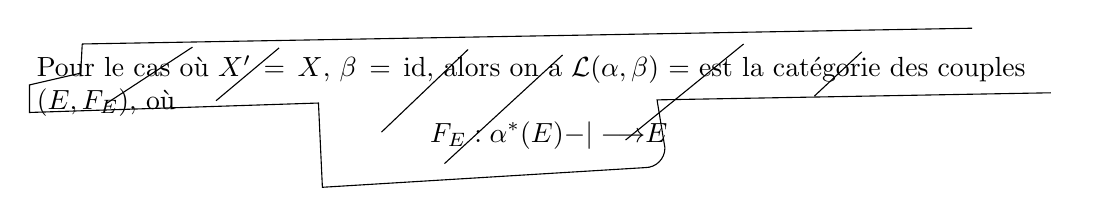
\begin{tikzpicture}[x=1cm,y=1cm]
\node[anchor=north west,text width=13cm,align=left] at (0,0) {\deleted{\unsure{Pour le cas où} $X'=X$, $\beta=\mathrm{id}$, alors \unsure{on a} $\mathcal L(\alpha,\beta)$ \deleted{\unsure{=}} est la catégorie des couples $(E,F_E)$, où
\[
F_E:\alpha^*(E)\unsure{-|\longrightarrow}E
\]}};
\draw (.7,.02)--(12,.22);
\draw (.7,.02)--(.68,-.35)--(.03,-.5)--(.03,-.85)--(3.7,-.73)--(3.75,-1.8)--(7.85,-1.55) to[out=0,in=-90] (8.1,-1.3)--(8.0,-.69)--(13,-.6);
\draw (1.0,-.74)--(2.1,-.02) (2.4,-.7)--(3.2,-.03) (4.5,-1.1)--(5.6,-.05) (5.3,-1.5)--(6.8,-.12) (7.6,-1.2)--(9.1,.02) (10,-.64)--(10.6,-.08);
\end{tikzpicture}}

Le \deleted{catégorie} \inserted{topos} $\mathcal L(\alpha,\beta)$ dépend ``fonctoriellement'' de
\diagram{\begin{tikzcd}[ampersand replacement=\&]\alpha,\beta:\quad X'\arrow[r,shift left]\arrow[r,shift right,dash]\&X\end{tikzcd}}
de façon précise, si on a un diagramme
\diagram{\begin{tikzcd}[ampersand replacement=\&]
u:\quad X'\arrow[r,shift left,"\alpha"]\arrow[r,shift right,dash,"\beta"']\arrow[d,"u_1"']\arrow[dr,phantom,"\unsure{\nearrow\ \nearrow|\xi\ \psi}" description]\&X\arrow[d,"u_0"]\\
Y'\arrow[r,shift left,"\lambda"]\arrow[r,shift right,dash,"\mu"']\&Y
\end{tikzcd}}
\margin{\unsure{a|u}}
\mspage{17}


\scanpage{19}
commutatif à isom près, on en déduit (p.ex. à l'aide de la caractérisation universelle de la prop) un \deleted{foncteur} \inserted{morphisme de topos}
\[
\mathcal L(u):\mathcal L(\alpha,\beta)\longrightarrow\mathcal L(\lambda,\mu)
\]
avec transitivité,\unsure{\ldots} rendant commutatif (à isom can. près) le diagramme
\diagram{\begin{tikzcd}[ampersand replacement=\&]
X\arrow[r,"\omega_X"]\arrow[d,"u_0"']\arrow[dr,phantom,"\overset{\sim}{\nearrow}" description]\&\mathcal L(\alpha,\beta)\arrow[d,"\mathcal L(u)=v"]\\
Y\arrow[r,"\omega_Y"']\&\mathcal L(\lambda,\mu)
\end{tikzcd}};
d'ailleurs les foncteurs $\mathcal L(u_0)_*$ et $\mathcal L(u_0)^*$ s'explicitent essentiellement comme indiqué au n°1, qu'on \deleted{\unsure{expl}} interprète \deleted{par le} en disant qu'on est dans le cas
\[
X'=X,\quad Y'=Y,\quad\beta=\mathrm{id}_X,\quad\mu=\mathrm{id}_Y,\qquad\alpha=f_X,\quad\lambda=f_Y,
\]
et en disant qu'on a un carré commutatif comme dessus\ldots\ldots

Revenons au cas général. Si $\mathcal E\inserted{=(E,F_E)}$ est un objet abélien de $\mathcal L(\alpha,\beta)$, on a des ``hom de chgt. de base''
\[
\omega_X^*(R^iv_*(\mathcal E))\longrightarrow R^iu_{0*}(\omega_X^*(\mathcal E))=R^iu_{0*}(E),
\]
et on aimerait savoir que ce sont des \uline{isoms}, sachant que c'est le cas pour $i=0$. On est obligé pratiquement d'établir que \deleted{\unsure{de}} si $\mathcal E\inserted{=(E,F_E)}$ est un faisceau abélien \uline{injectif} de $\mathcal L(\alpha,\beta)$, alors $E$ est un faisceau acyclique \deleted{\unsure{en}} (SGA4 V\quad). Il suffit pour ceci que $\alpha$ et $\beta$ commutent aux produits infinis (i.e. $\alpha_!$, $\beta_!$ existent)
\mspage{18}


\scanpage{20}
auquel cas il en est de $\overline{\mathrm m}$ de $\omega_X$ i.e $\omega_{X!}$ existe.
\mspage{19}


\scanpage{21}
\margin{\uline{\unsure{Th|Alg} de De Rham}\\(à puissances divisées)}
\mspage{20}


\scanpage{22}
\uline{\S1} Pseudo-anneau $=$ groupe abélien à loi de composition interne associative bilinéaire.

Nous sous-entendrons par la suite la commutativité.

Pseudo-anneau \inserted{$J$} \uline{à puissances} \uline{divisées}. C'est un ps-anneau muni d'applications \deleted{satisfaisant}
\[
\pi^n:x\rightsquigarrow x^{(n)}=\pi^n(x)\qquad n\in\mathbb N^+
\]
satisfaisant les conditions
\[
\begin{aligned}
1.1.\quad&\pi^1=\mathrm{id}\qquad\text{i.e.}\qquad x^{(1)}=x\\
1.2.\quad&\pi^n(x+y)=\deleted{\unsure{\sum}}\pi^n(x)+\sum_{\substack{p,q\ge1\\p+q=n}}\pi^p(x)\pi^q(y)+\pi^n(y)\\
1.3.\quad&\pi^n(xy)=x^n\pi^n(y)\\
1.4.\quad&\pi^m(\pi^n(x))=\frac{(mn)!}{(n!)^m m!}\pi^{mn}(x)\\
1.5.\quad&\pi^m(x)\pi^n(x)=\frac{(m+n)!}{m!n!}\pi^{m+n}(x)
\end{aligned}
\]
Supposons que $J$ est un idéal d'un anneau $A$, avec la structure de pseudo-anneau induite. Alors la relation 2. peut s'écrire
\[
\pi^n(x+y)=\sum_{p+q=n}\pi^p(x)\pi^q(y)\qquad x,y\in J
\]
où on pose $\pi^0x=1$, $\pi^p(x)=0$ si $p<0$. De la formule 5. on tire
\[
\text{(1.5.bis)}\qquad\pi^{p_1}(x)\pi^{p_2}(x)\cdots\pi^{p_r}(x)=\frac{(p_1+\cdots+p_r)!}{p_1!\cdots p_r!}\pi^{p_1+\cdots+p_r}(x)
\]
en particulier
\[
\text{1.\unsure{5|7}.ter}\qquad n!\pi^n(x)^{\deleted{\unsure{n}}}=\deleted{\unsure{n!}}x^n
\]
\unsure{Que|Si} $\Lambda$ est un anneau (comm), une $\Lambda$-algèbre
\mspage{21}


\scanpage{23}
à puissances divisées est un \inserted{pseudo-}\uline{anneau} à puissances divisées, muni d'une structure de $A$-algèbre, satisfaisant
\[
1.6.\qquad\pi^n(\lambda x)^{\unsure{n}}=\lambda^n\pi^n(x)\qquad\lambda\in A,\quad x\in\unsure{D|J}.
\]
\margin{N.B. C'est tjs vérifié si $\Lambda=\mathbb Z$}

Si $J$ est un idéal de $A$, c'est une $A$-algèbre; on \deleted{\unsure{dit que la structure à puissances divisées}\ \unsure{compatible}\ \illegible{2}\ \unsure{scalaires}} \inserted{appelle structure à puissances divisées sur \uline{l'idéal}} $J$ une structure de puissances divisées sur la \deleted{ps-anneau} \inserted{$A$-algèbre} sous-jacente, i.e. une structure de p.div. sur le pseudo-anneau sous-jacent, satisfaisant 6.

\uline{\S2} Soit $A$ un anneau, et $M$ un $A$-module. Considérons \inserted{la $A$-algèbre}
\[
\Gamma^*(M)=\coprod_{n\ge0}\Gamma^n(M),
\]
on a des applications
\[
\pi^n_{(1)}:x\rightsquigarrow x^{(n)}\qquad\text{de }M\text{ dans }\Gamma^nM
\]
On va les prolonger en des applications
\[
\pi^n:\Gamma^+(M)\longrightarrow\Gamma^+(M)\qquad x\rightsquigarrow x^{(n)}
\]
induisant
\[
\pi^n_{(p)}:\Gamma^p(M)\longrightarrow\Gamma^{np}(M)\qquad\deleted{\unsure{x\rightsquigarrow x^{(n)}}}
\]
en notant que ceci revient à se donner une ``application polynomiale homogène'' de degré $p$
\[
x\rightsquigarrow\pi^n_{(p)}(x^{(p)}):\underset{\sim}{M}\longrightarrow\underset{\sim}{\Gamma^{np}(M)}
\]
\inserted{``$(x^{(p)})^{(n)}$}
et on prendra
\[
(x^{(p)})^{(n)}=x^{(pn)}\frac{(pn)!}{(p!)^n n!}
\]
\mspage{22}


\scanpage{24}
On vérifie que les $\pi^n:\Gamma^+(M)\longrightarrow\Gamma^+M$ ainsi construits satisfont les conditions 1.1. à 1.6. ($\Gamma^+(M)$ considéré comme un idéal de $\Gamma(M)$, ou comme une $\Lambda$-algèbre).

$\Gamma^{\unsure{+|*}}(M)$ devient ainsi une $\Lambda$-algèbre à puissances divisées. Elle est munie d'un hom de $\Lambda$-modules
\[
M\longrightarrow\Gamma^+(M)\ ;
\]
ce \unsure{dernier} \unsure{joue} un rôle \uline{universel}.

\uline{§ 3} Soit $A$ un anneau, et $I$ un idéal de $A$. On s'intéresse, --- pour un anneau $B$, muni d'un idéal $J$ \uline{à puissances divisées}, aux homs d'anneaux
\[
u:A\longrightarrow B
\]
tels que $u(I)\subset J$. On cherche un tel \unsure{fourbi|fonct.}, \uline{universel}. On prend l'\deleted{\unsure{anneau}} \inserted{$A$-algèbre} $\Gamma^{\unsure{+|*}}(A,\unsure{I|J})$ engendré par des éléments
\[
\pi^n x\qquad \deleted{n\in\unsure{\mathbb N^{*}|\mathbb N}}\inserted{n\geq2},\ x\in\unsure{I|J}
\]
avec les relations 1.2. à 1.6. (où \deleted{\unsure{i}} $x,y\in\unsure{I|J}$, $\lambda\in A$, et $\pi^1(x)$ doit être $x$). Une autre façon de le dire est celle-ci: $\unsure{I|J}$ est un $A$-module, on construit $\Gamma_A^+(\unsure{J|I})$, et on
\mspage{23}


\scanpage{25}
divise \deleted{\unsure{cet}} \inserted{pseudo-}anneau à puissances divisées par l'idéal engendré par les
\[
(x.y)^{(n)}-x^n*y^{(n)}
\]
où le signe $*$ désigne provisoirement la multiplication de $\Gamma_A^+(J)$, le $.$ celle de $J$. On constate que les opérations $\pi^n$ passent au quotient \inserted{$J'$} pour donner une structure \inserted{de $A$-algèbre} à puissances divisées sur $J'$ [construction indépendante du fait que $J$ est un idéal de $A$]. On considère maintenant l'extension de $A/J$ par \inserted{la $A$-algèbre} $J'$ déduite de $J\longrightarrow J'$, i.e. le quotient
\[
A\times J'/\alpha(J^{\unsure{\flat|b}}),\quad\text{où}\qquad
\alpha:J^{\unsure{\flat|b}}\longrightarrow A\times J'
\]
est donné par
\[
\alpha(x)=(x,-x')
\]
où $x\sim x'$ est l'application canonique $J\longrightarrow J'!$

\deleted{On a, si $\deleted{\unsure{(a,X)}}\ (a,\unsure{\zeta|\xi})\in A\times J'$}

On \deleted{$(a,\unsure{\zeta|\xi})(x,-x')=ax,-\unsure{\zeta|\xi} x$} \unsure{je gue.}

\uline{N.B.} Supposons que $A$ soit une algèbre sur un anneau $\Lambda$. Alors le composé $\Lambda\longrightarrow A-\Gamma(A,J)$ définit évidemment sur $\Gamma(A,J)$ une structure de $\Lambda$-algèbre.
\mspage{24}


\scanpage{26}
\uline{Cas particulier}

$A=\operatorname{Sym}_{\Lambda}(M)$ où $M$ est un $\Lambda$-module

\deleted{$\unsure{M}$} $J=\operatorname{Sym}_{\Lambda}^{+}(M)$ l'idéal d'augmentation.

Alors le pb universel est le même que celui d'envoyer $\underline{M}$ dans une $\Lambda$-algèbre à puissances divisées, on trouve
\[
\Gamma(\operatorname{Sym}_{\Lambda}(M),\operatorname{Sym}_{\Lambda}^{+}(M))\simeq\Gamma_{\Lambda}^{\unsure{+|*}}(M)
\]
Ainsi, en tant qu'algèbre \deleted{\unsure{de $\Lambda$-anneau}} à puissances divisées $\Gamma_{\Lambda}(M)$ dépend fonctoriellement de l'anneau \uline{augmenté} $\operatorname{Sym}_{\Lambda}^{\unsure{+|*}}(M)$ \unsure{---}

\deleted{Si $A=\Lambda[T_1,\ldots,T_n]$}

\margin{plus haut au § 1, aux fonctorialités\ldots}

\margin{\unsure{\S\,1}} [Soit $A$ un \deleted{$\Lambda$-algèbre} \inserted{anneau avec idéal $J$} à puissances divisées, considérons des éléments $(x_i)_{i\in I}$ \inserted{de $J$} et proposons-nous de \unsure{trouver} les homs $(A,J)\longrightarrow(A'',J'')$ avec $A'$ un \deleted{$\Lambda$-algèbre} \inserted{anneau à idéal $J'$} à puissances divisées, qui annulent les $x_i$. Existe-t-il un $(A',J')$ universelle? Oui, il suffit de prendre le quotient de $A$ par l'idéal \inserted{$K$} engendré par les $\pi^n(x_i)$ $i\in I$, $n\geq1$, i.e. les expressions
\[
\sum \deleted{(\unsure{\lambda_i})}\deleted{\unsure{\lambda}}(\lambda_{ni}\,\pi^n(x_i)),\quad\inserted{\text{avec}}\deleted{(\unsure{\lambda_i\pi^n(x_i)})}
\]
\deleted{$\unsure{\lambda_i,\lambda}$} $\lambda_{ni}\in A$. On \unsure{trouve} ainsi le plus petit idéal $K$ stable par les $\pi^n$ $(n\geq1)$,
\mspage{25}


\scanpage{27}
contenant les $x_i$, et pour un idéal $K$ stable \inserted{(et pour un tel seulement)}, les $\pi^n$ passent au quotient et définissent sur $(A/K,J/K)$ une structure d'anneau à idéal avec puiss. divisées.]

Anneau avec idéal à puissances divisées \uline{$n$-tronqué}: qui satisfait
\[
\deleted{\unsure{(x)}}\quad x^{(i)}=0\quad\text{pour }i>\unsure{n|m},\ x\in J
\]
ce qui implique que
\[
x\in J\Longrightarrow x^{n+1}=0
\]
Si $J$ est engendré par un nb fini d'éléments $x_1---x_N$, tous ceux-ci sont nilpotents, $J$ est un \uline{nilidéal} [de façon précise, $J^{Nn+1}=0$]. \deleted{Application}

Anneau ``avec'' \uline{nilidéal à puissances divisées \deleted{``nilpotentes}} \deleted{$\forall x,\exists n$} $\exists n$, tel \deleted{\unsure{que}} qu'il soit \deleted{tronqué} à puissances divisées $n$-tronquées. Anneau ``avec idéal à puissances divisées nilpotentes'', $\forall x$, $\exists n$ tel que $x^{(i)}=0$ si $i>n$. On a, pour un tel anneau, deux isom de groupes inverses l'un de l'autre

\diagram{\begin{tikzcd}[ampersand replacement=\&,column sep=huge,row sep=large]
1+J \arrow[r,shift left=1.0ex,"\log(1+x)=\sum_{\unsure{n>0|n\geq0}}(-1)^n(n-1)!x^{(n)}"] \& J \arrow[l,shift left=1.0ex,"\exp x=\sum_{n\geq0}x^{(n)}"] \\
A^* \arrow[u,phantom,"\cap" description] \&
\end{tikzcd}}
\mspage{26}


\scanpage{28}
§ 4 \uline{Site de De Rham}

\diagram{\begin{tikzcd}[ampersand replacement=\&]
 \& U \arrow[r,phantom,"\subset" description] \& X \arrow[dd,"f"] \\
U' \arrow[ur] \& \& \\
 \& \& S
\end{tikzcd}}

Schéma relatif. Les objets du \uline{site de De Rham} \inserted{$(X/S)_{\mathrm{DR}}$, ou $\mathrm{DR}(X/S)$} sont les \deleted{triplets} \inserted{quadruples} \deleted{$(U,\mathcal A,\varphi,\pi^*)$}\inserted{$(U,U',i,\pi)$}, où $U$ est un ouvert de $X$, \deleted{$\mathcal A$ un faisceau \unsure{de} $i:U\longrightarrow U'$} $U'$ un $S$-préschéma, $i:U\longrightarrow U'$ une $S$-imm. nilpotente, et $\pi$ une structure de puissances divisées tronquées (pour $n$ convenable) sur $J=\operatorname{Ker}(\underline{O}_{U'}\unsure{-|\longrightarrow}\underline{O}_U)$. Morphismes du site évidents. Topologie itou: la ``topologie de Zariski''.

Le site de \uline{De Rham restreint} (ou \inserted{\uline{site de De Rham}} \uline{\unsure{stratifiant|strictifiant}}) est formé des objets tels que localement sur $U'$ il \uline{existe} une rétraction sur $U$ (N.B. cette rétraction n'entre pas dans la structure).

Topos. $\widetilde{(X/S)}_{\mathrm{DR}}$; $\widetilde{(X/S)}_{\mathrm{DRst}}$ ou \deleted{simplement} $\widetilde{\mathrm{DR}}(X/S)$, $\widetilde{\mathrm{DRst}}(X/S)$; si une ambiguïté n'est pas à craindre, on laisse tomber le $/S$.

Diagramme de morphismes de topos
\mspage{27}


\scanpage{29}
\diagram{\begin{tikzcd}[ampersand replacement=\&]
\deleted{\unsure{\widetilde X_{\mathrm{DR}}|\widetilde{\mathrm{Zar}}(X)}} \arrow[r] \& \deleted{\unsure{\widetilde{\mathrm{DR}}(X)}} \arrow[r] \& {}
\end{tikzcd}}

\diagram{\begin{tikzcd}[ampersand replacement=\&]
\widetilde{\mathrm{Zar}}(X) \arrow[r,dashed] \& \widetilde{\mathrm{DRstrat}}(X) \arrow[r] \arrow[d] \& \widetilde{\mathrm{Strat}}(X) \arrow[d] \\
 \& \widetilde{\mathrm{DR}}(X) \arrow[r] \& \widetilde{\mathrm{Cris}}(X)
\end{tikzcd}}

Si $X$ est \unsure{formt.} lisse sur $S$, alors les flèches verticales sont des équivalences de Topos. Si $X$ est de car. 0, (p.ex. $S$ de car. 0) alors les flèches horizontales sont des équivalences de Topos.

Dans les sites $\mathrm{DR}(X)$ et $\mathrm{DRst}(X)$, les produits fibrés (de deux objets sur un troisième) et les noyaux de couples existent. Mais il semble douteux que ce soit le cas pour \unsure{ces} $\mathrm{Cris}(X)$ et $\mathrm{Strat}(X)$ \ldots
\margin{?}

\figure{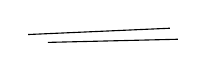
\begin{tikzpicture}\draw (0,0)--(1.8,0.08);\draw (0.25,-0.1)--(1.9,-0.06);\end{tikzpicture}}

Travaillons dans $\mathrm{DRstrat}(X)$. Notons que l'objet $\widetilde X$ de $\widetilde{\mathrm{DRst}}$ associé à $X$ couvre l'objet final (par définition des objets de $\mathrm{DRstrat}$). Donc on peut utiliser \deleted{$\mathrm{DRstrat}$} $\widetilde X$ pour écrire une suite spectrale de Leray
\[
H^*(X_{\mathrm{DRst}},O)\Longleftarrow E_2^{pq}=H^p(\unsure{\nu|\gamma}\longmapsto H^q(\widetilde X^{\unsure{\nu|\gamma}+1},O))
\]
\mspage{28}


\scanpage{30}
Or $\widetilde X^{\nu+1}$ est ind-représentable de la façon suivante. On regarde sur $X^{(\nu)}:=X^{\nu+1}$ les voisinages infinitésimaux $\Delta_{X/S}^{(\nu)}(i)$ de la diagonale. Pour chacun, on regarde (grâce à l'augmentation $\underline O_{\Delta^{(\nu)}(i)}\longrightarrow O_{\Delta^{(\nu)}(\unsure{0|\omega})}=\underline O_X$) le \unsure{fourbi|fonct.} augmenté à \uline{puissances divisées} qu'il définit, soit $\widetilde{\Delta_{X/S}^{(\nu)}(i)}$ [\deleted{\unsure{ainsi on}} c'est une notation \unsure{doublement} justifiée, i.e. cohérente avec \deleted{celle déjà} l'usage de $\sim$ déjà utilisé\ldots], et ses $j$-tronqués [\deleted{pour} \deleted{$j$} \deleted{le} au sens des puissances divisées] $\Delta_{X/S}^{(\nu)}(i,j)$, de sorte que du point de vue
\[
\underbrace{\widetilde{\Delta_{X/S}^{(\nu)}(i)}}_{\begin{gathered}
\text{faisceau}\\
\deleted{\text{De Rham}}\ \mathrm{DR}\text{-stratifiant}\\
\text{``\deleted{\unsure{ind}}représenté'' par }\Delta_{X/S}^{(\nu)}(i)\text{ augmenté}\\
\text{\unsure{vers}}\quad\Delta_{X/S}^{(\nu)}\deleted{\unsure{(i)}}(\unsure{0|\omega})
\end{gathered}}
=\varinjlim_j\Delta_{X/S}^{(\nu)}(i,j)
\]
et
\[
\widetilde X^{\unsure{2\nu+1|\nu+1}}=\varinjlim_{i,j}\widetilde{\Delta_{X/S}^{(\nu)}(i,j)}.
\]
On aura aussi
\[
H^q(\widetilde{\mathrm{DRst}}/\widetilde{(U,U')},O)\simeq H^q(U',\underline O_{U'})
\]
\margin{à vérifier}
\mspage{29}


\scanpage{31}
pour tout objet $U'$ du site \inserted{DR-}stratifiant. D'où, si $X$ est affine
\[
\left\{\begin{aligned}
H^q(\widetilde X^{\nu+1},O\unsure{]|)}&=0\quad\text{si }q>0\\
H^0(\widetilde X^{\nu+1},O)&=\varprojlim_{i,j}H^0(\Delta_{X/S}^{(\nu)}(i,j),O_{\Delta_{X/S}^{(\nu)}(i,j)})
\end{aligned}\right.
\]
et par suite
\[
H^n(X_{\mathrm{DRstrat}},O)\simeq H^n(\nu\longmapsto H^0(\widetilde{\widehat{X^{\nu+1}}_{/X}}))
\]
Dans le cas général, on trouve sur $X$ un anneau cosimplicial $\underline O_X$-augmenté à puissances divisées, soit $\mathcal E^*$, et
\[
H^*(X_{\mathrm{DRstrat}},O)\simeq\mathbb H^*(X_{\mathrm{zar}},\mathcal E^*)
\]
\mspage{30}


\scanpage{32}
Soit $A$ un anneau, $I$ idéal de $A$, \deleted{$(x_i)_{i\in I}$ un syst. de gén. de $I$}. On cherche \deleted{\unsure{un}} $B$ avec idéal $J$ à puiss. divisées, et hom $A\overset{u}{\unsure{-|\longrightarrow}}B$ avec $u(I)\subset J$, qui soit \uline{universel}. On prend l'algèbre quotient
\[
B=A[\deleted{\unsure{\Gamma_i^n}}\{\Gamma_{\deleted{x}}^n(x)\}_{\substack{x\in\unsure{J|I}\\n\geq2}}\}]/\ \deleted{\unsure{les}}\ \text{relations}
\]
\[
\left\{\begin{aligned}
&\Gamma^n(x+y)-(\Gamma^n x+\Gamma^n y+\sum_{\substack{p,q\geq1\\p+q=n}}\Gamma^p(x)\Gamma^q(y))\quad x,y\in I;\quad\text{où }\Gamma_x^1=x\ \inserted{\text{par déf.}}\\
&\Gamma^n(xy)-x^n\Gamma^n(y)\qquad x\in I,\ y\in A\\
&\deleted{\Gamma^{\unsure{n|m}}(\Gamma^{\unsure{m|n}}(x))-\frac{(mn)!}{\unsure{n!(m!)^n|(n!)^m m!}}\Gamma^{mn}(x)}\\
&\Gamma^m(x)\Gamma^n(x)-\frac{(m+n)!}{m!n!}\Gamma^{m+n}(x)\qquad x\in I
\end{aligned}\right.
\]
\margin{\unsure{où}} \uline{$J$} idéal engendré par les $\Gamma^n(x)$ $(n\geq1,x\in\unsure{J|I})$.

\deleted{\unsure{Supposons que} \illegible{5}}

Vérifions que c'est une solution au Pb universel. Il faut introduire sur $J$ des puiss. div\ldots

\deleted{Pour cela \unsure{on voit que l'on} \unsure{le fait} \illegible{2} \unsure{clair que} de prendre $\Gamma_{\unsure{A|\Lambda}}(J)$ ($J$ étant considéré comme $A$-module) \unsure{et on le} divise par l'idéal engendré par les $\deleted{\unsure{\Gamma^n(xy)}}(xy)^{(n)}-x^n*y^{(n)}$, où $*$ est produit}

Supposons qu'on ait un nb premier $p$ tel que tous les $l\ne p$ soient inv. dans $A$, \inserted{i.e. $A$ une alg. sur $\mathbb Z_{p\mathbb Z}$} Alors on peut simplifier la construction de $B$, en notant que si $n$ est un entier, sous forme $p$-adique \deleted{\unsure{soit}}
\[
n=a_0+a_1p+a_2p^2---+a_\nu p^\nu\qquad0\leq a_i\leq p-1,
\]
alors on aura
\[
\nu_p(n)=\sum a_i\nu_p(p^{\unsure{\nu|i}})\qquad[\mathrm{NB}\ \nu_p(p^\nu)=\frac{p^\nu-1}{p-1}]
\]
d'où \deleted{si $C$ est} un $A$-alg. avec idéal $K$ à puiss. divisées, pour tt $x\in K$
\[
\gamma^n(x)=\deleted{\unsure{\frac{\gamma^n(x)}{n!}}\ \unsure{a}}\ C_n\,\deleted{\unsure{x^0}}\gamma^1(x)^{a_0}\gamma^p(x)^{a_1}---(\gamma^{p^\nu}(x))^{a_\nu}
\]
où $C_n\in\mathbb Z_{p\mathbb Z}$ est donné par
\mspage{31}


\scanpage{33}
\[
C_n=\frac{\prod_i[(p^i!)/p^{\nu_p(p^i!)}]^{a_i}}{[n!/p^{\nu_p(n!)}]}=\text{partie première à }p\text{ de }\frac{\prod(p^i!)^{a_i}}{n!}
\]
Par suite, $B$ est aussi engendré par les images des $\Gamma^{p^\nu}(x)$, $\nu\geq1$,\inserted{$x\in I$,} qu'on va noter $[x,\nu]$.

Quelles sont les relations?

\uline{Définissons} les $\Gamma^n(x)$ dans $A[\deleted{\unsure{\Gamma}}\{[x,\nu]\}_{\substack{x\in I\\\nu\geq1}}]$ par la formule ci-dessus, \inserted{donc $\Gamma^{p^\nu}(x)=[x,\nu]$,} on trouve les \deleted{formules} \inserted{relations}
\[
\deleted{\unsure{\Gamma_x^{p^\nu}}}\quad\deleted{[x,\nu]}
\]
\margin{ne faut-il en passer par les $\Gamma^n(x+y)$, tous $n$?}
\[
\left\{\begin{aligned}
\Gamma^{p^\nu}(x+y)&=\Gamma^{p^\nu}x+\Gamma^{p^\nu}y+\underbrace{\sum_{\substack{\alpha,\beta\geq1\\\alpha+\beta=p^\nu}}\deleted{\unsure{\Gamma^\beta}}\Gamma^\alpha(x)\Gamma^\beta(y)}_{\substack{\text{expression en les}\\\Gamma^{p^i}(x),\Gamma^{p^j}(y),\ i,j<\nu}}\\
\Gamma^{p^\nu}(xy)&=x^{p^\nu}\Gamma^{p^\nu}(y)\\
\Gamma^{\unsure{p^m}}(x)\Gamma^{\unsure{p^n}}(x)&=\frac{(p^m+p^n)!}{p^m!p^n!}\Gamma^{p^m+p^n}(x)\quad\ldots
\end{aligned}\right.
\]
\margin{\unsure{il suffit de} ? \unsure{en poser} pour certains $m,n$. On se demande s'il suffit
$\Gamma^{p^\nu}(x)^p=\dfrac{(p^{\nu+1})!}{(p^\nu!)^p}\Gamma^{p^{\nu+1}}(x)$}

\figure{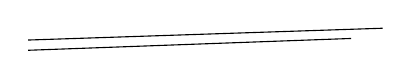
\begin{tikzpicture}\draw (0,0)--(4.5,0.15);\draw (0,-0.13)--(4.1,0.02);\end{tikzpicture}}

Supposons maintenant que $I$ soit engendré par un élément $\lambda$. Alors $B$ est aussi \deleted{\unsure{un}} le quotient de $A[(\Gamma^n(\lambda))_{n\geq2}]$ par les relations
\mspage{32}


\scanpage{34}
\mspage{41}
$\underline a=\sum_i m_i(a_i)\in Z(A)$, on posera $\underline q_{\underline a}=\prod_i m_i\,\underline q_{a_i}$. On a toujours $\operatorname{div}(\underline q_{\underline a})=(\operatorname{div}\underline q)_{\underline a}$. Pour $\underline a\in Z_o(A)$, et $v\in M_{\overline K}$, le nombre réel $\underline q_o(\underline a,v)$ ne dépend que de $\underline q$, $\underline a$, et $v$. Nous le désignerons par $\underline q(\underline a,v)$.

\margin{\figure{\begin{tikzpicture}[x=1cm,y=1cm]\draw[gray,line width=.2pt] (0,1.2) -- (1.2,1.65);\draw[gray,line width=.2pt] (0,0) .. controls (.8,-.12) and (1.3,-.16) .. (1.7,-.06);\end{tikzpicture}}}
Soit $X\in D_\ell(V)_{\overline K}$, et soit $f$ une fonction sur $V$, définie sur $\overline K$, telle que $\operatorname{div}(f)=X$. La classe $\chi_V(f)$ de la quasi-fonction principale $\widetilde f$ ne dépend que de $X$. Cette classe sera désignée par $\underset{\sim}{f}(X)$, ou $\underset{\sim}{f}_V(X)$.

Soit $A$ une variété abélienne définie sur $K$. Nous noterons $Q^*_\ell(A)$ (resp. $Q^*_a(A)$) le sous-groupe de $Q^*(A)$ composé des éléments $\underline q$ tels qu'on ait $\operatorname{div}(\underline q)\in D_\ell(A)$ (resp. $\operatorname{div}(\underline q)\in D_a(A)$).

Pour $\underline q\in Q^*_\ell(A)$, nous poserons $\xi_o(\underline q)=\underset{\sim}{f}(\operatorname{div}(\underline q))\,q^{-1}$. On a $\operatorname{div}(\xi_o(\underline q))=0$, d'où $\xi_o(\underline q)\in B^*(A)$, et il est clair que l'application $\xi_o:Q^*_\ell(A)\longrightarrow B^*(A)$ ainsi définie est un homomorphisme. Pour $u\in A_{\overline K}$, l'homomorphisme $\xi_o$ commute avec la translation $\tau_u$; autrement dit, pour $\underline q\in Q^*_\ell(A)$, on a $\xi_o(\underline q_u)=(\xi_o(\underline q))_u$. Montrons en outre que, pour $\underline q\in Q^*(A)$, et pour $\underline a$, $\underline b$ $Z_o(A)$, tels qu'on ait $X_{\underline a}$ et $X_{\underline b^-}\sim0$ (i.e. $\underline q_{\underline a}$ et $\underline q_{\underline b}\in Q^*_\ell(A)$), on a les relations
\[
(15)\qquad (\xi_o(\underline q_{\underline a}))(\underline b,v)=(\xi_o(\underline q_{\underline b^-}))(\underline a^-,v)=(\xi_o(\underline q^-_{\underline b}))(\underline a,v).
\]
En effet, soit $f$ une fonction sur $A$, définie sur $\overline K$, et admettant pour diviseur $X_{\underline a}$. Soit d'autre part $\underline r$ une quasi-fonction sur $A$ représentant $\underline q$. On a
\[
\begin{aligned}
(\xi_o(\underline q_{\underline a}))(\underline b,v)&=(\widetilde f\,r_{\underline a}^{-1})(\underline b,v)\\
&=(\widetilde f\,r_{\underline a}^{-1})_{\underline b^-}(0,v).
\end{aligned}
\]
\mspage{33}


\scanpage{35}
\[
\left\{\begin{aligned}
\alpha)\quad&\Gamma^m(\lambda)\Gamma^n(\lambda)-\frac{\unsure{(m+n)!|(m+n!}}{m!n!}\Gamma^{m+n}(\lambda)\\
\alpha*)\quad&\deleted{\unsure{x^n\Gamma^n(\lambda x)-y^n\Gamma^n}}\quad(x^n-y^n)\Gamma^n(\lambda)\quad\text{pour }x,y\in A\ \inserted{\text{tels que}}\ (x-y)\lambda=0.
\end{aligned}\right.
\]
[ \uline{NB} On récupère $\Gamma^n(\lambda x)$ comme $\equiv x^n\Gamma^n(\lambda)$,
qui \deleted{ne} ne dépend en effet que de $\lambda x$ --- \unsure{ici|car} \deleted{\unsure{on a}} $\lambda x=\lambda y$ implique $x^n\Gamma^n(\lambda)\equiv y^n\Gamma^n(\lambda)$;
\margin{grâce à $(\alpha*)$}
les relations $\Gamma^n(\lambda(x+y))\inserted{\equiv\ldots}$ résultent alors des $\alpha$,
$\Gamma^n(xy)\equiv x^n\Gamma^n(y)$ est trivial, ainsi que $\Gamma^{\unsure{n|m}}(\lambda x)\Gamma^{\unsure{m|n}}(\lambda y)=\ldots$.

Si maintenant tous les nbs premiers $\ne p$ sont inv., on trouve aussi le quotient de $\unsure{A|\Lambda}[(\Gamma^{p^\nu}(\lambda))_{\nu\geq1}]$ par les relations
\[
\left\{\begin{aligned}
&\Gamma^m(\lambda)\Gamma^n(\lambda)-\frac{\unsure{(m+n)!|(m+n!}}{m!n!}\Gamma^{m+n}(\lambda)\\
&(x^n-y^n)\Gamma^n(\lambda)\qquad\text{si }x,y\in A\text{ tels que }(x-y)\lambda=0
\end{aligned}\right.
\]
où $\Gamma^n(\lambda)$ se définit en termes des $\Gamma^{p^\nu}(\lambda)$ comme plus haut. Les premières relations se réduisent, semble-t-il, à
\[
\boxed{\Gamma^{p^\nu}(\lambda)^{\unsure{p+a|p^a}}=\deleted{\unsure{\Gamma^{p^{\nu+1}}\frac{(a+b)!}{}}}\quad\frac{(\unsure{a|e}p^{\nu+1})!}{(p^\nu!)^p}\Gamma^{\unsure{a|e}p^{\nu+1}}(\lambda)}
\]
pour $p\leq e\unsure{<|\leq}2p-1$, donc pour $e=p+a$ $(0\leq a\leq p-1)$

à $\Gamma^{p^\nu}(\lambda)$
\mspage{34}


\scanpage{36}
\mspage{39 bis}
\margin{\figure{\begin{tikzpicture}[x=1cm,y=1cm]\draw[gray,line width=.2pt] (0,1) -- (1.2,1.45);\draw[gray,line width=.2pt] (0,0) .. controls (.7,-.08) and (1.2,-.16) .. (1.55,-.09);\end{tikzpicture}}}
fini ($\varepsilon$ et $m_o$ fixés). Il en résulte aussitôt que la suite $\psi(m)$ est de Cauchy, donc convergente.

Soit $a$ la limite de cette suite. En remplaçant la suite donnée $\varphi(m)$ par la suite $\varphi(m)-am$, on se ramène au cas où cette limite $a$ est nulle; autrement dit, il nous suffit de prouver que, dans ce dernier cas, on a nécessairement $|\varphi(m)|\leq d$ pour tout $m$. Or on a, d'après la relation (14), $|\varphi(2m)-2\varphi(m)|\leq d$; plus généralement, pour tout entier $h>0$, on en déduit, par récurrence sur $h$, $|\varphi(2^hm)-2^h\varphi(m)|\leq(2^h-1)d$. Donc, s'il existait un $m_1$ tel que $\varphi(m_1)=d_1>d$, on aurait $\varphi(2^hm_1)>(2^h-1)(d_1-d)$, et $\psi(2^hm_1)=\varphi(2^hm_1)/2^hm_1$ ne tendrait pas vers $0$ pour $h$ infini. Ceci contredirait l'hypothèse $a=0$.
\mspage{35}
\figure{\begin{tikzpicture}\draw (0,0)--(0.02,-0.22);\end{tikzpicture}}


\scanpage{37}
Lemme de Poincaré vrai pour les $k$-algèbres suivantes ($k$ corps de car. nulle).
\[
\left\{\begin{aligned}
&k[[x]][\unsure{Y|X}]/(Y^p-x^q)\\
&k[[x]][Y]/(Y^2+P(x)Y+Q(x))\\
&k[x_1,\ldots x_n]/(x_1^{p_1},x_2^{p_2},\ldots,x_n^{p_n})\qquad\text{p. ex. }k[x]/(x^p)\\
&k[x,y]/\mathfrak m^2\\
&k[x,y]/(x^3,y^2,x^2y)\\
&k[x,y]/(x^3,y^2,xy)
\end{aligned}\right.
\]
Si $A$ \deleted{\unsure{Artinien}} local sur $k$, ext. résiduelle triviale, alors pour tt $x\in\mathfrak m$ avec $d_{A/k}x=0$, on a $x\in\mathfrak m^3$.

\figure{\begin{tikzpicture}
\node[anchor=west] at (0,0) {Ann. Éc. N. Sc.};
\node[anchor=west] at (4.3,0.13) {$65\ \unsure{ou|à}\ 66$};
\node[anchor=west] at (0.4,-0.65) {ou};
\node[anchor=west] at (1.6,-0.65) {J. de Liouville};
\draw (4.15,0.4)--(4.1,-0.14)--(5.9,-0.14);
\draw (5.85,0.4)--(6.02,0.4)--(5.96,-0.75)--(5.79,-0.75);
\draw (5.89,0.38)--(5.84,-0.73);
\end{tikzpicture}}
\mspage{36}


\scanpage{38}
\mspage{-18-}
effet, les réductions successives de la preuve de (6.14.4) ramènen\inserted{t,} \uline{sans utiliser} (6.14.1), au cas où $C$ est \inserted{/} \uline{intègre}, $A$ le corps des fractions de $C$. Comme alors $B$ est un anneau normal et que le morphisme $\operatorname{Spec}(B')\longrightarrow\operatorname{Spec}(B)$ est \uline{étale}, il résulte de (17.5.7) que $B'$ est un anneau \deleted{\unsure{noethérien}} normal; le raisonnement se termine \deleted{\unsure{alors}} en faisant appel seulement au lemme élémentaire \deleted{\illegible{1}} (6.14.1.1), mais non à la partie difficile de la preuve de (6.14.1).
\mspage{37}


\scanpage{39}
\uline{Supposons que les car. résiduelles de $A$} \uline{soient \unsure{égales|positives}:} $p>0$
\[
\deleted{(x^{\unsure{(n)}})^{(m)}=}\qquad\text{op. de puiss. div. }(\pi_n)_{n\geq0}
\]
a)
\[
\pi_m^{\deleted{(m)}}(a)\pi_n^{\deleted{(n)}}(a)=\binom{m+n}{n}\pi_{m+n}^{\deleted{(m+n)}}(a)
\]
Supposons que $\left\{\begin{aligned}m&\equiv0\ (p)\\0&\leq n\leq p-1\end{aligned}\right.$ alors
\[
\deleted{\unsure{\pi^m}}\quad\binom{m+n}{n}=\frac{(m+1)\cdots(m+n)}{n!}\not\equiv0\ (p)
\]
donc
\[
\boxed{\pi_{m+n}^{\deleted{(m+n)}}(a)=\binom{m+n}{n}^{-1}\pi_m^{\deleted{(m)}}(a)\pi_n^{\deleted{(n)}}(a)}
\]
b)
\[
\pi_m^{\deleted{m}}\circ\pi_n^{\deleted{n}}=\frac{(mn)!}{(n!)^m m!}\pi_{mn}^{\deleted{mn}}
\]
[ Supposons $m=p$, on trouve un coefficient
\[
c_n=\frac{(pn)!}{(n!)^p p!}
\]
et on a, si $n=a_0+a_1p+\cdots+a_rp^r$
\[
\begin{aligned}
\nu_p(c_n)&=\deleted{\unsure{a}}\ \nu_p((pn)!)-p\nu_p(\unsure{m|n}!)-1\\
&=\frac{pn-\sum a_i}{p-1}-p\frac{n-\sum a_i}{p-1}-1\\
&=\deleted{\frac{1}{p-1}}(\sum a_i)-1
\end{aligned}
\]
]
\figure{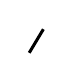
\begin{tikzpicture}\draw[line width=1.1pt] (0,0)--(0.18,0.3);\end{tikzpicture}}
Supposons $n=p$, on trouve un coeff.
\[
d_m=\frac{(pm)!}{(p!)^m m!}
\]
\margin{$m=\deleted{\sum}b_0+b_1p+\cdots+b_sp^s$}
et
\[
\begin{aligned}
\nu_p(d_m)&=\nu_p((pm)!)-m\nu_p(p!)-\nu_p(m!)\\
&=\frac{pm-\sum b_i}{p-1}-m-\frac{m-\sum b_i}{p-1}\\
&=0
\end{aligned}
\]
donc
\[
\pi_{pm}^{\deleted{pm}}=\left(\frac{(pm)!}{(p!)^m m!}\right)^{-1}\pi_m^{\deleted{m}}\circ\pi_p^{\deleted{p}}
\]
a) et b) ensemble nous montrent que \uline{les} $\pi_n^{\deleted{n}}$ \uline{sont connus} \uline{quand on connaît} $\pi_p^{\deleted{p}}$
\mspage{38}


\scanpage{40}
\mspage{39}
\mspage{-4}
\uline{Professeur Nicolaas H. Kuiper}: \textit{Variétés Hilbertiennes}

\uline{Programme}

Variétés Hilbertiennes; aspects géométriques.

Les sujets qui seront traités sont les suivants:

\uline{Introduction}: Définition d'une variété $X$, modelée sur un espace de Banach, de classe de différentiabilité $C^r$. (Le livre de Serge Lang: ``Introduction to differentiable manifolds'' sera supposé connu de l'auditoire). (There is a cheaper french version of the book).

Théorème de Bessaga: L'espace de Hilbert $H$ est (analytiquement) difféomorphe à $H-\{0\}$.

Construction d'un plongement fermé de $X$ dans $B$. Par exemple pour $B=c_o\oplus\unsure{l|1}_p$. Existence d'une norme $C^\infty$ sur l'espace , $c_o$ des suites convergeant vers $0$.

Le groupe linéaire d'un espace de Hilbert est contractile.

Le théorème d'isotopie ambiante des voisinages tubulaires.

La version, en dimension infinie, du théorème d'isotopie ambiante de Hirsch et quelques lemmes simples de transversalité.

Fonctions non dégénérées sur une variété hilbertienne, condition $C$ de Palais-Smale. Forme canonique d'une telle fonction au voisinage d'un point critique. Théorème d'existence de Nicole Moulis. Décomposition en anses. Théorie de Morse. Stabilité d'après Palais: la variété Hilbertienne $X$ est difféomorphe à $X\,x\,H$. Enoncé du théorème de plongement ouvert de Eells et Elworthy.

\margin{$\ldots/$}


\scanpage{41}
$\pi=\pi^p$ satisfait les conditions
\[
\left\{\begin{aligned}
\pi^{\deleted{p}}(x+y)&=\pi x+\pi y+\sum_{0<i<p}\deleted{\unsure{C_i^p}}\frac{1}{i!(p-i)!}x^iy^{\unsure{i}}\\
\pi(fx)&=f^p\pi x
\end{aligned}\right.
\]
Si on a une application satisfaisant ces conditions, peut on définir les $\pi^{(n)}$ \deleted{?} satisfaisant les conditions \deleted{\unsure{premières}} \inserted{des puiss. div.} $(1.1):(1.5)$?, avec $\pi^{\unsure{(p)}}=\pi$

\deleted{On \unsure{construira|construit} les $\pi_N$ par récurrence, en supposant les $\pi_i$ construits pour $i<N$ et \unsure{de façon à} satisfaire $(1.1):(1.5)$ [les $\unsure{1.4|1.5}$ pour $mn<N$, les $1.5$ pour $m+n<N$].

\uline{Cas} $1$\quad $N\not\equiv0\ (p)$ donc $N=N'+\deleted{\unsure{p}}s$, avec $N'\equiv0\ (p)$, $0<s\leq p-1$.

On aura donc $\ldots$}

On va construire
\[
\pi_n(x)=c_nx^{a_0}\pi(x)^{a_1}\pi^2(x)^{a_2}\cdots\pi^r(x)^{a_r}
\]
où
\[
n=a_0+a_1p+\cdots+a_rp^r
\]
est le développement $p$-adique de $n$, et où \deleted{\unsure{c}}
\[
\deleted{c_n\in\mathbb Z\cap\mathbb Z_p^*}\qquad c_n\in\mathbb Q\cap\mathbb Z_p^*
\]
est un élément de $\mathbb Q$ dont la valuation $p$-adique est nulle.

[ Il serait intéressant de connaître $c_n$ mod $p$, qui est un élément de $\mathbb F_p^*$. Est-ce tjs $1$? ].
\mspage{40}


\scanpage{42}
\mspage{41}
\mspage{-3}
6- Coefficients locaux et ``isomorphisme de Thom''.

7- Suites exactes de catégories de Banach.

8-9- Description des groupes $\unsure{k|K}^{p,q}(X)$ à l'aide d'opérateurs de Fredholm. Structures multiplicatives. Espaces classifiants.

10- K-théorie équivariante.

11- Applications diverses de la K-théorie.

N.B.- En principe, aucune connaissance spéciale de K-théorie n'est requise pour suivre cette série de conférences. Cependant, on pourra utilement consulter les exposés de K-théorie du Séminaire Cartan 1963/1964, et les notes aux comptes-rendus, t. 263, série A, p. 275, 347 et 357 et t. 267, même série, p. 305, 328 et 345. (voir aussi l'exposé de Cartan au séminaire Bourbaki 1968/1969).

\uline{Professeur Joseph J. Kohn}: \textit{Complexes différentiels}.

\uline{Programme}

The lectures will concentrate on differential complexes which are not elliptic. The main example of interest is the case of the Cauchy-Riemann equations (the \quad- complex) restricted to a real submanifold. The course will be planned to complement the courses given by Kuranishi and Spencer. If time permits various boundary value problems will also be discussed. Every effort will be made to make the course accessible to all who have had a basic graduate course in analysis.

\margin{$\ldots/$}


\scanpage{43}
Une application polynomiale homogène \inserted{de degré $n$} $\Phi:\underset{\sim}{M}\longrightarrow\underset{\sim}{N}$ définit par la formule
\[
\Phi\left(\sum_1^r t_ix_i\right)=\sum_{p_1+\cdots+p_r=n}\Phi_{p_1\cdots p_r}(x_1,\ldots,x_r)t_1^{p_1}\cdots t_r^{p_r}
\]
[les $t_i$ des indéterminées] des applications polynomiales
\[
\Phi_{p_1\cdots p_r}:\quad\unsure{\underset{\sim}{M}|\underline M}\times\cdots\times\underline M\unsure{\longrightarrow|\mathrel{\text{---}}}\underline N
\]
multihomogènes de degrés $p_1,\ldots,p_r$, d'où des applications
\[
\varphi_{p_1,\ldots,p_r}:\quad\underbrace{M\times\cdots\times M}_{r}\longrightarrow N
\]
(définies si $r\geq1$, $p_1,\ldots,p_r\geq0$, $\sum p_i=n$). Ces applications sont reliées par des relations
\[
\varphi_{p_1,\ldots,p_r}\deleted{\unsure{\varphi}}\left(\sum_{1\leq i\leq s_1}x_{1,i},\ \sum_{1\leq i\leq s_2}x_{2,i},\ \ldots\sum_{1\leq i\leq s_r}x_{r,i}\right)
=\sum_{\left\{\substack{\sum_{1\leq i_1\leq s_1}q_{1,i_1}=p_1\\\sum_{1\leq i_2\leq s_2}q_{\unsure{1|2},i_2}=p_2\\\cdots\\\sum_{1\leq i_r\leq s_r}q_{r,\unsure{s_r|i_r}}=p_r}\right.}
\varphi_{q_{1,i_1},\ldots,q_{r,s_r}}(x_{11},\ldots,\unsure{x_{r,s_r}}
\]
\margin{\figure{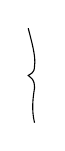
\begin{tikzpicture}[x=.4cm,y=.4cm]\draw (0,3) .. controls (.1,2.6) and (.25,2.1) .. (.2,1.8) .. controls (.2,1.55) and (.05,1.55) .. (0,1.5) .. controls (.1,1.4) and (.2,1.4) .. (.2,1.1) .. controls (.15,.8) and (.1,.4) .. (.2,0);\end{tikzpicture}}il suffit quand \uline{un} des \unsure{argts|arguments} est \unsure{remplacé} par une somme de \uline{deux} termes}
\uline{Plus relations de symétrie.}

On suppose que l'on a \unsure{une|aussi} réciproque $\ldots\ldots$
\mspage{42}


\scanpage{44}
b) $v_1$ et $v_2$ représentent, par abus de langage, les actions de $v_1\in V_1$ et de $v_2\in V_2$ sur $E$.

c) $v_1\cos\theta+\varepsilon^i\sin\theta$, $i=1,2$, $\theta\in[0,\pi/2]$, représentent, encore par abus de langage, les graduations $v_1\cos+\varepsilon^i\sin\theta$ au point de $S^+(V_1+1)$ de coordonnées $v_1\cos\theta+\varepsilon\sin\theta$, $v_1$ appartenant à $S(V_1)$ et $\varepsilon$ représentant le vecteur unité de $R$.

\uuline{Théorème 1.1} $^{(2)}$: L'homomorphisme
\[
t:K^{V_1+V_2}(X)\longrightarrow K^{V_2}(B(V_1),S(V_1))
\]
est un isomorphisme.

1.4\quad Soit $\operatorname{Spin}(p,q)$ le sous-groupe du groupe multiplicatif $(C^{p,q})^*$ formé des éléments $x$ de degré zéro tels que
\[
\begin{aligned}
\text{a)}\quad&\forall\ y\in R^{p+q},\quad xyx^{-1}\in R^{p+q}\\
\text{b)}\quad&x^*x=1,
\end{aligned}
\]
$*$ désignant l'antiinvolution de $C^{p,q}$ définie sur les générateurs $e_i$, $i=1,\ldots,p+q$, par $e_i^*=-e_i$.
Pour un élément $x$ de $\operatorname{Spin}(p,q)$ la transformation $\sigma(x)$ définie par $\sigma(x)y=xyx^{-1}$ appartient en fait à $\operatorname{SO}(p,q)$ et on a une suite exacte
\diagram{\begin{tikzcd}[ampersand replacement=\&]
0\arrow[r]\&Z_2\arrow[r]\&\operatorname{Spin}(p,q)\arrow[r,"\sigma"]\&\operatorname{SO}(p,q)\arrow[r]\&0
\end{tikzcd}}
Pour plus d'informations sur le groupe $\operatorname{Spin}(p,q)$, voir $^{(2)}$.

Soit maintenant $V$ un fibré vectoriel réel muni d'une forme quadratique non dégénérée de type $(q,p)$, i.e. dont le groupe structural est réduit à $\operatorname{O}(p,q)$. On dira que le fibré $V$ est spinoriel de type $\operatorname{Spin}(p,q)$ si on se donne un fibré principal $P$ de groupe $\operatorname{Spin}(p,q)$ tel que $V\approx P\,x_{\operatorname{Spin}(p,q)}R^{p+q}$, $\operatorname{Spin}(p,q)$ opérant sur $R^{p+q}$ par la représentation $\sigma$. Si $\mathcal C$ est une catégorie de Banach arbitraire, on définit maintenant une équivalence de catégories
\mspage{43}


\scanpage{45}
\figure{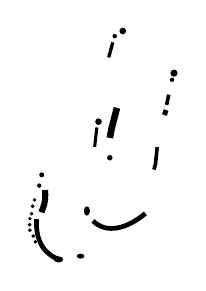
\begin{tikzpicture}[x=.35cm,y=.35cm]
\draw[line width=1.2pt] (3.0,8.6)--(3.15,9.15);
\fill (3.22,9.37) circle (.08); \fill (3.51,9.56) circle (.12);
\fill (5.37,8.03) circle (.13); \fill (5.30,7.79) circle (.08);
\draw[line width=1.3pt] (5.18,7.25)--(5.10,6.88);\draw[line width=1.8pt] (5.08,6.69)--(5.02,6.51);
\draw[line width=2.4pt] (3.30,6.77)--(3.11,6.04)--(3.04,5.68);
\draw[line width=1.1pt] (2.57,6.06)--(2.49,5.35);\fill (2.63,6.27) circle (.12);\fill (3.04,4.96) circle (.10);
\draw[line width=1.3pt] (4.76,5.35)--(4.70,4.74)--(4.64,4.53);
\fill (.57,4.34) circle (.09);\fill (.48,3.95) circle (.08);
\draw[line width=2.2pt] (.69,3.79) .. controls (.73,3.29) and (.60,3.13) .. (.56,2.98);
\foreach \x/\y in {.31/3.43,.24/3.20,.20/2.93,.14/2.75,.13/2.53,.14/2.33,.26/2.12,.34/1.91} {\fill (\x,\y) circle (.07);}
\draw[line width=1.7pt] (.38,2.73) .. controls (.34,1.90) and (.69,1.41) .. (1.28,1.25);
\fill (1.18,1.27) ellipse (.17 and .11);\fill (1.98,1.39) ellipse (.14 and .09);
\draw[line width=1.7pt] (2.43,2.67) .. controls (2.92,2.18) and (3.67,2.39) .. (4.33,2.94);
\fill (2.21,3.03) ellipse (.11 and .17);
\end{tikzpicture}}
\uline{Cristaux}
\margin{\illegible{1}\quad \unsure{C}\illegible{1}\quad \unsure{C}\illegible{1}\unsure{n}\quad \illegible{1}\quad \unsure{C}\illegible{1}\unsure{n}\quad \unsure{C}\illegible{1}\unsure{on}}

Soit $J$ un idéal principal d'un anneau $A$, $J=\pi A$. Formellement, pour y définir des puissances divisées, on est amené à définir des
\[
\frac{(\pi y)^n}{n!}=\frac{\pi^n}{n!}y^n=\pi^{(n)}y^n
\]
\margin{\illegible{1}\quad \unsure{C}\illegible{1}\quad \illegible{1}\quad \unsure{Canson|CANSON}\quad \illegible{1}\quad \unsure{Canson|CANSON}}
donc à définir des éléments
\[
\pi^{(0)}=1\qquad\deleted{\unsure{et}}\quad\pi^{(n)}\in\pi A\qquad(n\geq1)
\]
qui satisfassent aux conditions suivantes.
\margin{\unsure{Canson|CANSON}\quad \unsure{Canson|CANSON}\quad \unsure{C}\illegible{1}\unsure{n}\quad \unsure{Canson|CANSON}\quad \unsure{C}\illegible{1}\unsure{n}\quad \unsure{Canson|CANSON}}
\figure{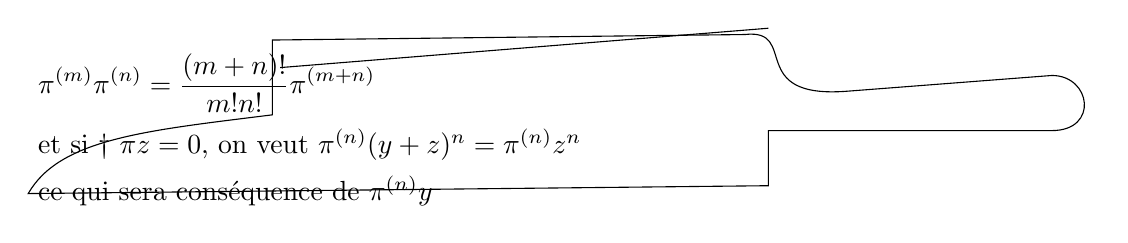
\begin{tikzpicture}[x=1cm,y=1cm]
\node[anchor=north west,text width=13cm,align=left] at (0,0) {\deleted{$\displaystyle\pi^{(m)}\pi^{(n)}=\frac{(m+n)!}{m!n!}\pi^{(m+n)}$}\\[5pt]\deleted{et si $\unsure{\dagger}$ $\pi z=0$, on veut $\pi^{(n)}(y+z)^n=\pi^{(n)}z^n$}\\[5pt]\deleted{ce qui sera conséquence de $\pi^{(n)}y$}};
\draw (3.1,.05)--(9.1,.12) .. controls (9.8,.2) and (9.1,-.7) .. (10.4,-.6)--(13,-.4) .. controls (13.5,-.4) and (13.6,-1.1) .. (13,-1.1)--(9.4,-1.1)--(9.4,-1.8)--(0,-1.9) .. controls (.4,-1.2) and (1.5,-1.1) .. (3.1,-.9)--cycle;
\draw (3.2,-.3)--(9.4,.2);
\end{tikzpicture}}
\[
\pi^{(1)}=\pi
\]
\margin{\unsure{Canson|CANSON}\quad \unsure{C}\illegible{1}\quad \illegible{1}\quad \illegible{1}\quad \unsure{Canson|CANSON}\quad \unsure{Canson|CANSON}}
\[
\unsure{\alpha|a}\quad\left\{\begin{aligned}
\pi^{(m)}\pi^{(n)}&=\frac{\unsure{(m+n)!|(m+n!}}{m!n!}\pi^{(m+n)}\\
\pi^{(p)}\left(\frac{\pi^{(q)}}{\pi}\right)^p&=\frac{(pq)!}{p!(q!)^p}\pi^{(pq)}.
\end{aligned}\right.
\]
\uline{NB} Comme $\pi^{(q)}\in\pi A$, $\dfrac{\pi^{(q)}}{\pi}$ est défini mod. addition d'un $z$ tel que $\pi z=0$, mais comme $\pi^{(p)}\in\pi A$, on détermine sans ambiguïté l'élément $\pi^{(p)}\left(\dfrac{\pi^{(q)}}{\pi}\right)^p$.

\margin{\illegible{1}\unsure{on}\quad \illegible{1}\quad \illegible{1}\unsure{n}\quad \illegible{1}\unsure{n}\quad \illegible{1}\unsure{on}\quad \unsure{C}\illegible{1}\unsure{on}}

Alors on trouve une structure de puissances divisées \inserted{de $I=\pi A$} en posant
\[
x^{(n)}=(\pi y)^{(n)}=\pi^{(n)}y^n\qquad\text{pour }x=\pi y\in J,
\]
\margin{\illegible{1}\unsure{on}\quad \unsure{Canson|CANSON}\quad \unsure{Canson|CANSON}\quad \unsure{C}\illegible{1}\quad \unsure{C}\illegible{1}\unsure{on}\quad \illegible{1}\unsure{on}}
en notant que $x^{(n)}$ ne dépend pas du choix de $y$ \unsure{t.q.|d.q.} $x=\pi y$.

\uline{Exemple$^1$} Supposons que $A$ soit sans torsion sur $\mathbb Z$. Alors les \deleted{\unsure{premières}} relations
\[
\pi^n=n!\pi^{(n)}
\]
\margin{\illegible{1}\quad \illegible{1}\quad \illegible{1}\quad \unsure{C}\illegible{1}}
déterminent uniquement les $\pi^{(n)}$ en fonction de $\pi$, et leur existence équivaut au fait que $\pi^n\in n!A\quad\forall n\geq2$. Les relations $\unsure{\alpha|a}$ sont satisfaites automatiquement.

\uline{Exemple$^2$} Supposons $A_o=\mathbb Z_{(p\mathbb Z)}$, \deleted{Alors} $\pi=p$. Alors les conditions précédentes sont satisfaites,
\margin{\unsure{Canson|CANSON}\quad \unsure{C}\illegible{1}\unsure{on}\quad \illegible{1}\quad \unsure{C}\illegible{1}\quad \illegible{1}}
les $\dfrac{p^n}{n!}$ sont des entiers p-adiques. Donc si $A$ est un anneau dans lequel tout nb premier $q\ne p$ est inv. (i.e. les seules car. résiduelles sont $p,0$), \unsure{i.e.} une algèbre sur $A_o$, on trouve par spécialisation des $\pi^{(n)}\in A$, $\pi^{(n)}=\dfrac{p^n}{n!}$, qui
\margin{\illegible{1}\quad \illegible{1}\quad \illegible{1}}
\mspage{44}


\scanpage{46}
\mspage{- IV-977 -23-}

\unsure{ïncide} avec le module de différentielles analytiques défini dans (18.13.1) ; \deleted{\illegible{4}} \inserted{en effet} (les définitions étant celles de (18.13.1)), il résulte du fait que $\overline{\Omega}^{1}_{A/k}$ est de type fini \deleted{\illegible{1}} et de (\uline{0},20.4.8) que \deleted{\illegible{12}} la dérivation $\overline{d}_{A/k}$ se factorise en \deleted{\illegible{3}} $A\xrightarrow{d_{A/k}}\Omega^1_{A/k}\xrightarrow{u_0}\overline{\Omega}^1_{A/k}$ et que tout A-homomorphisme \deleted{\illegible{1}} $\Omega^1_{A/k}\xrightarrow{u}L$, où L est un A-module de type fini, se factorise nécessairement en $\Omega^1_{A/k}\xrightarrow{u_0}\overline{\Omega}^1_{A/k}\xrightarrow{v}L$, si bien que $\operatorname{Ker}(u)$ contient toujours $\operatorname{Ker}(u_0)$, d'où notre assertion.

On notera que \uline{si} $\overline{\Omega}^1_{B/A}$ est un B-module \uline{de type fini}, il \uline{représente} le foncteur covariant $L\rightsquigarrow\operatorname{Dér}_A(B,L)$ dans la catégorie des B-modules \uline{de type fini}. \deleted{\illegible{4}} Il est clair que si $\Omega^1_{B/A}$ lui-même est \uline{de type fini} (ce qui sera par exemple le cas (\uline{0},20.4.7) lorsque B est une A-algèbre \uline{de type fini}), on a $\overline{\Omega}^1_{B/A}=\Omega^1_{B/A}$.

\uline{Proposition} (18.13.5).-- \uline{Soient} A \uline{un anneau topologique}, \deleted{\illegible{2}} \inserted{B \uline{et} C \uline{deux}} \uline{A-algèbres topologiques qui} \deleted{\illegible{1}} \inserted{\uline{sont des}} \uline{anneaux} \deleted{\illegible{10}} \uline{semi-locaux noethériens et dont les topologies sont les topologies préadiques}, $\rho:B\to C$ \uline{un A-homomorphisme continu. Alors} :

\figure{\begin{tikzpicture}\draw (0,0.7) .. controls (1.1,0.2) and (-0.2,-0.8) .. (0.2,-0.7) .. controls (1.6,1.3) and (4.8,1.3) .. (4.9,0.6) .. controls (5.1,-0.4) and (3.7,-0.6) .. (3.3,0) .. controls (2.5,-0.4) and (2.1,-0.6) .. (1.8,-0.4);\end{tikzpicture}}

(i) \uline{Si} \deleted{\unsure{C est un B-module}\illegible{5}} $\overline{\Omega}^1_{C/A}$ \uline{est un C-module de type fini} \deleted{\illegible{1}} $\overline{\Omega}^1_{C/B}$ \uline{est un C-module de type fini}.

(ii) \uline{Si} $\overline{\Omega}^1_{B/A}$ \uline{est un B-module de type fini et si} C \uline{est une B-algèbre finie}, $\overline{\Omega}^1_{C/A}$ \uline{est un C-module de type fini}.

(iii) \uline{Supposons vérifiées, soit les hypothèses de} (ii), \uline{soit} \deleted{\illegible{2}} \uline{l'hypothèse de} (i) \uline{et la condition supplémentaire que} $\Omega^1_{B/A}$ \uline{est un B-module de type fini ; alors il existe deux C-homomorphismes} \deleted{\uline{déterminés de} \inserted{façon} \uline{unique}}, $\overline{u}:\overline{\Omega}^1_{C/A}\to\overline{\Omega}^1_{C/B}$ \uline{et} \deleted{\unsure{:}} $\overline{v}:\overline{\Omega}^1_{B/A}\otimes_B C\to\overline{\Omega}^1_{C/A}$ \uline{tels que le diagramme}
\margin{style \uline{ambigu}}
\figure{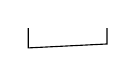
\begin{tikzpicture}\draw (0,0.2)--(0,-0.05)--(1,0)--(1,0.2);\end{tikzpicture}}

\diagram{\begin{tikzcd}[ampersand replacement=\&,column sep=large]
\Omega^1_{B/A}\otimes_B C \arrow[r,"v"] \arrow[d,"r'\otimes1"'] \& \Omega^1_{C/A} \arrow[r,"u"] \arrow[d,"r"'] \& \Omega^1_{C/B} \arrow[r] \arrow[d,"r''"] \& 0 \\
\overline{\Omega}^1_{B/A}\otimes_B C \arrow[r,"\overline{v}"'] \& \overline{\Omega}^1_{C/A} \arrow[r,"\overline{u}"'] \& \overline{\Omega}^1_{C/B} \arrow[r] \& 0
\end{tikzcd}}
\margin{(18.13.5.1)}
\margin{45}


\scanpage{47}
\unsure{satisfont} aux conditions précédentes $\unsure{\alpha)}$, donc une structure à puissances divisées canonique sur $pA$.

\uline{Exemple} 3 \quad Soit $A$ intègre, \deleted{\unsure{à valuation}} tel que les seules \deleted{\unsure{son corps des fractions soit}} \unsure{car.} résiduelles soient $p$ et $0$. Soit $\pi$ un élément tel que les caractéristiques résiduelles de $A/\pi A$ soient $p$. À quelle condition peut-on trouver des $\unsure{\pi^{(n)}|\pi^{[n]}}$ ?

Supposons que $A$ soit de valuation discrète. Il faut écrire \deleted{$\unsure{\forall}$} $\pi^n/n!\in A$, i.e.
\[
v(\pi^n/n!)\geq 0\qquad\text{pour }\forall n
\]
i.e.
\[
n v(\pi)-v(n!)\geq0\qquad\text{pour tout }n.
\]
Soit \deleted{$\unsure{v_p}$} $v(p)=e$ l'indice de ramification absolue de $A$, \unsure{on a} \deleted{$v(N)$} pour $\forall$ entier $N$,
\[
v(N)=e\,v_p(N).
\]
\deleted{Soit de plus $\rho=v(\pi)$.} La condition s'écrit
\[
\deleted{\unsure{\rho}}v(\pi)\geq\deleted{\unsure{e}}e\frac{\deleted{\unsure{e}}v_p(n!)}{n}\deleted{\unsure{e}}\qquad\text{pour tout }n
\]
i.e.
\[
v(\pi)\geq e\lambda(p)\qquad\text{où}\quad\lambda(p)=\sup_n\frac{v_p(n!)}{n}\inserted{=\frac1{p-1}}
\]
\margin{\unsure{Legendre}}
est une constante ne dépendant que de $p$, et qui est $\leq1$ \ldots\ Donc on trouve la condition
\margin{\deleted{\unsure{déterminer} $\lambda(p)$}}
\[
v(\pi)\geq\frac{e}{\unsure{r|p}-1}.
\]
Supposons que $\pi$ soit l'uniformisante, donc $v(\pi)=1$, on trouve la condition
\[
\boxed{e\leq p-1}
\]
\margin{46}


\scanpage{48}
\mspage{- IV-977 -22-}

(18.13.4) Le résultat de (18.13.2), \deleted{joint au fait que pour une k-algèbre analytique A, $\overline{\Omega}^1_{A/k}$ soit un A-module de type fini}, peut encore s'exprimer en disant que dans la catégorie des A-modules \uline{de type fini}, $\overline{\Omega}^1_{A/k}$ est un objet \uline{représentant le foncteur covariant} $L\rightsquigarrow\operatorname{Dér}_{\unsure{k|A}}(A,L)$ \inserted{($\uline{0}_{\mathrm{III}}$,8.1.11)}.

\figure{\begin{tikzpicture}\draw (0,0.2) .. controls (-0.1,-0.2) and (0.6,-0.2) .. (1,-0.2)--(4.5,-0.2) .. controls (4.8,-0.2) and (4.8,-0.3) .. (4.8,-0.5);\end{tikzpicture}}

Nous allons généraliser ce résultat. Considérons d'abord un anneau topologique A, et une A-algèbre topologique B qui est un \uline{anneau semi-local noethérien, muni de sa topologie $\underline r$-préadique} ($\uline{r}$ étant le radical de B). Alors, pour tout B-module \uline{de type fini} L, toute A-dérivation D de B dans L est \uline{continue} pour les topologies $\underline r$-préadiques sur B et L, puisque l'on a $D(\underline r^{j+1})\subset\underline r^jL$ pour tout entier j ; en vertu de (\uline{0},20.4.8) elle s'écrit donc $D=u\circ d_{B/A}$, où $u:\Omega^1_{B/A}\to L$ est un homomorphisme de B-modules (nécessairement \uline{continu} pour les topologies $\underline r$-préadiques, et on sait que dans le cas considéré la topologie \inserted{canonique} de $\Omega^1_{B/A}$ est la topologie \deleted{\illegible{2}} \inserted{$r$-préadique} ((\uline{0},20.4.5)). Nous désignerons par $\overline{\Omega}^1_{B/A}$ le quotient de $\Omega^1_{B/A}$ par l'\uline{intersection des noyaux des homomorphismes} $\Omega^1_{B/A}\to L$ pour les B-modules \inserted{L} \uline{de type fini} (ou, ce qui revient au même puisque \deleted{\illegible{1}} L est noethérien, l'intersection des sous-modules M de $\Omega^1_{B/A}$ tels que $\Omega^1_{B/A}/M$ soit \uline{de type fini}). \inserted{On a donc $\operatorname{Hom}_B(\overline{\Omega}^1_{B/A},L)=\operatorname{Hom}_B(\Omega^1_{B/A},L)$ pour tout B-module de type fini L.} Nous désignerons par $\overline d_{B/A}$ ou simplement $\overline d$ l'application composée $B\xrightarrow{d_{B/A}}\Omega^1_{B/A}\xrightarrow{r}\overline{\Omega}^1_{B/A}$ ; c'est une \inserted{A-}dérivation, et $\overline{\Omega}^1_{B/A}$ est engendré par les éléments $\overline d_{B/A}(x)$ où x parcourt B, en vertu de (\uline{0},20.4.7) ; la définition précédente montre que l'application $v\rightsquigarrow v\circ\overline d_{B/A}$ est un isomorphisme de B-modules, fonctoriel en L
\margin{*}
\figure{\begin{tikzpicture}\draw (0.4,0.6) .. controls (-0.2,0.2) and (-0.3,-0.5) .. (0,-0.5) .. controls (1.6,0.1) and (0.7,0.8) .. (0.4,0.6);\draw (0.7,-0.15) .. controls (0.7,-0.7) and (2.4,-0.5) .. (2.4,0.35) .. controls (2.4,0.6) and (2.25,0.7) .. (2.15,0.7);\draw (6,0.7) .. controls (4.7,0.5) and (4.9,-0.3) .. (5.2,-0.3) .. controls (6.6,-0.2) and (6.7,0.6) .. (6,0.7);\end{tikzpicture}}
\margin{à quoi servent ces hypothèses ? Prendre un anneau topologique plus général ?}
\[
(18.13.4.1)\qquad \operatorname{Hom}_B(\overline{\Omega}^1_{B/A},L)\xrightarrow{\sim}\operatorname{Dér}_A(B,L)\inserted{=\operatorname{Dér.cont}_A(B,L)}
\]
L étant toujours supposé \uline{de type fini}. \deleted{\illegible{1}} Lorsque l'on est dans les conditions de (18.13.2), le A-module $\overline{\Omega}^1_{A/k}$ qui vient d'être défini co-
\margin{47}


\scanpage{49}
\margin{Lettre \unsure{Deligne}\par sur coh. p-adiques}
\margin{48}


\scanpage{50}
\margin{10.12.1965}

Cher Deligne,

\figure{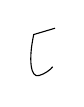
\begin{tikzpicture}[x=0.1cm,y=0.1cm]\draw (3,6)--(0.3,5.2)..controls(-0.4,2)and(-0.1,-0.4)..(1,0)..controls(1.7,0.2)and(2.4,0.7)..(2.7,1.1);\end{tikzpicture}}
Je vous propose une simplification pour la démonstration du théorème de dualité, qui permet d'éviter tout recours au théorème de pureté relative. Vous vous rappelez qu'on était réduit au cas où $f:X\quad Y$ est de dimension relative 1, $F=A_X$ et $G=A_Y$. Le procédé de passage à la limite de Exp VI, par.6, permet de supposer la base noethérienne, et même si on y tien de dimension finie (car de type fini sur $\underline Z$). On raisonne par récurrence sur $n=\dim X$. Si $n=0$, on sait le vérifier. Supposons le théorème démontré en dimension $<n$. Se localisant sur Y, on peut supposer Y strictement local. Alors, si y est son point fermé, on a $\dim(Y-y)\quad n$, et comme on est réduit à prouver le théorème séparément pour $X\times_Y(Y-y)$ et $X\times_Y y$, on gagne. - Autre remarque: le théorème de dualité peut se démontrer, essentiellement de la même façon et avec le même énoncé, pour un morphisme lisse $f:X\quad Y$ compactifiable, lorsque Y est muni d'un faisceau d'anneaux A quelconque tel que il existe un entier n premier aux caractéristiques \unsure{résidueales|résiduelles} annulant A, et X d'un faisceau d'\unsure{anneaux|anneaus} B, et f étant donné comme morphisme de (X,B) dans (Y,A), de sorte qu'on a un \inserted{homo}morphisme de faisceau d'anneaux $f^{-1}(A)\quad B$. On définit alors
\[
f^{!}(K^{\bullet})=R\,\underline{\operatorname{Hom}}^{\bullet}_{f^{-1}(A)}(B,f^{-1}(K)\otimes T_{X/Y}\quad 2d).
\]
La définition de l'homomorphisme trace et la démonstration du théorème de dualité se décomposent alors en le cas où $f^{-1}(A)\quad B$ est un isomorphisme, qui se traite comme le cas $A=(\underline Z/n\underline Z)_Y$, et le cas où $f=\operatorname{id}$, qui est trivial. Je pense qu'il vaut le coup d'inclure cette forme générale du théorème de dualité, soit de prime abord, soit à la fin dans un numéro-ratrappage. Je n'ai pas regardé si par hasard il pourrait se déduire du cas particulier
\margin{49}


\scanpage{51}
$A=(\underline Z/n\underline Z)_Y$ comme simple corollaire, mais ça m'étonnerait. La même remarque s'applique d'ailleurs également au théorème de dualité globale, qui s'énonce pour des faisceaux d'anneaux plus généraux que le faisceau constant $\underline Z/n\underline Z$.
\figure{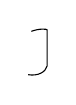
\begin{tikzpicture}[x=0.1cm,y=0.1cm]\draw(0,5.5)..controls(1,5.9)and(2,5.8)..(2,5.7)--(2,1.1)..controls(1.8,0.3)and(0.8,-0.2)..(-0.4,0);\end{tikzpicture}}

Il me semble que la relation de nature transcendante qui lie la cohomologie de De-Rham ou de Hodge aux cohomologies $\ell$-adiques, lorsque le corps de base est $\underline C$, via la cohomologie entière, devrait avoir un\deleted{\unsure{e relati|relati}}\deleted{\unsure{on|en}} analogue lorsque le corps de base est \inserted{alg clos} valué complet non archimédien, à corps résiduel de caractéristique p, \deleted{\unsure{caractéristique}} et corps des fractions \inserted{K} de caractéristique zéro,savoir que $H^*(X,\underline Z_p)$ doit s'envoyer alors de façon $\underline Z_p$-linéaire dans la cohomologie de De\unsure{-}Rham $H^*(X)$, qui serait isomorphe alors à $H^*(X,\underline Z_p)\otimes_{\underline Z_p}K$. Pour définir un tel homomorphisme, on pourrait penser à utiliser l'espace rigide-analytique au sens de Tate défini par X (NB c'est un site qui ne peut être défini par une topologie au sens ordinaire, ce qui explique les difficultés conceptuelles initiales de Tate pour arriver à définir la notion d'espace rigide-analytique), soit $X^{\mathrm{an}}$. On espère que les arguments habituels prouveront que pour des fais\deleted{\unsure{ce}}ceaux de torsion, la cohomologie de $X_{\text{ét}}$ coïncide avec celle de $X^{\mathrm{an}}$, et un excès d'optimisme nous ferait espérer que la cohomologie de $X^{\mathrm{an}}$ à coéfficients constants $\underline Z_p$ est bien la limite projective des cohomologies à coéfficients dans les $\underline Z/p^n\underline Z$, donc coïncide avec la cohomologie p-adique $H(X_{\text{ét}},\underline Z_p)$ (définie précisément comme une limite analogue). Si cela était vrai, l'immersion canonique de $\underline Z_p$ dans les fonctions constantes sur $X^{\mathrm{an}}$ semblerait permettre d'envoyer $H(X^{\mathrm{an}},\underline Z_p)$ dans la cohomologie de De Rham de $X^{\mathrm{an}}$, qui par Gaga rigide-analytique n'est autre que celle de X. L' ``excès'' plus haut serait justifié essentiellement par un ``lemme
\margin{50}


\scanpage{52}
de Poincaré'' rigide-analytique, disant que sur $X^{\mathrm{an}}$, le complexe de De-Rham est bien une résolution du faisceau des fonctions constantes à valeurs dans le corps de base. Notez bien que c'est certainement trivial pour l'analytique p-adique ordinaire, étant une simple question de séries converge\deleted{\unsure{a}}ntes dans \unsure{ce} cas, mais que la question pour la topologie rigide-analyique (qui est \unsure{beamucoup|beaucoup} plus grossière) est plus délicate. Je vous avoue d'ailleurs que j'ai de grands doutes que les choses marchent aussi simplement que ça, i.e. que la cohomologie rigide-analytique à coéfficients constants tout bêtes donne les ``bons'' nombres de Betti. Je crois me rappeler que Tate \unsure{m'avait|n'avait} dit que c'était déjà faux pour le $H^1$ des courbes elliptiques - il faudrait lui demander quel était son argument; apparemment, on trouverait un peu plus que pour la cohomologie étale, mais quand même pas toute la cohomologie. Il reste plausible néanmoins, quoi qu'il en soit, que la topologie rigide-analytique aura son rôle à jouer dans ces questions.

Notez qu'en caractéristique $p>0$, on a un homomorphisme évident de $H^*(X,\underline F_p)$ dans la cohomologie de De-Rham, comme on voit en calculant cette dernière pour la cohomologie étale et non pour la cohomologie de Zariski (ce qui donne le même résultat, puisque les composantes du complexe de De Rham sont quasi-cohérents), et utilisant la suite spectrale en cohomologie étale
\[
H^*(X)\Longleftarrow H^p(X,\underline H^q(\underline\Omega)).
\]
Cet homomorphisme se factorise d'ailleurs à travers $H^*(X,F_p)-H^*(X,\underline O_X)$, ce dernier s'envoyant dans $H^*(X)$ grace à l'homomorphisme de puissance p-ème $f\rightsquigarrow f^p$, induisant un isomorphisme $\unsure{\underline O_X|\underline\Omega_X}\simeq\underline H^0(\underline\Omega)$. Le composé des homomorphismes canoniques $H^{\deleted{\unsure{p}}\inserted{n}}(X,\underline O_X)\to H^n(X)\to H^n(X,\underline O_X)$ (ce dernier
\margin{51}


\scanpage{53}
résultant de l'autre suite spectrale pour la cohomologie de De Rham) ne peut guère être autre chose que l'homomorphisme de Frobenius. Il faut dire que tout ça est bien éculé, et qu'on ne pourra dire \deleted{\unsure{dans|des}} des choses vraiment intéressantes et nouvelles qu'en faisant appel à la ``\unsure{vraie|vcaie}'' cohomologie p\unsure{-}adique.

Bien cordialement
\margin{52}


\cotefile{6}
\scanpage{1}
IMAG

INSTITUT MONTPELLIERAIN

ALEXANDER GROTHENDIECK

\figure{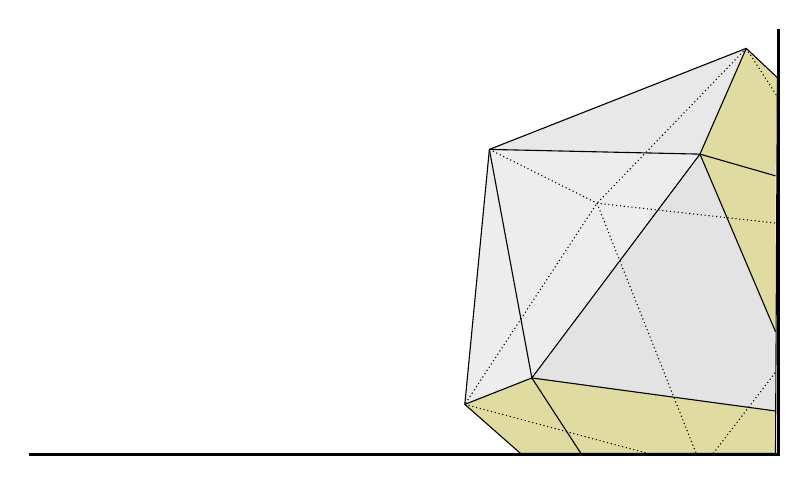
\begin{tikzpicture}[x=0.012cm,y=-0.012cm]
\fill[gray!18] (497,138)--(769,31)--(720,143)--cycle;
\fill[gray!14] (497,138)--(720,143)--(542,380)--(471,408)--cycle;
\fill[gray!22] (720,143)--(800,331)--(800,415)--(542,380)--cycle;
\fill[olive!28] (769,31)--(802,62)--(800,166)--(720,143)--cycle;
\fill[olive!28] (720,143)--(800,166)--(800,331)--cycle;
\fill[olive!28] (471,408)--(542,380)--(800,415)--(800,460)--(530,460)--cycle;
\draw (497,138)--(769,31)--(802,62)--(800,460)--(530,460)--(471,408)--cycle;
\draw (497,138)--(720,143)--(769,31);
\draw (720,143)--(800,166);
\draw (720,143)--(800,331);
\draw (497,138)--(542,380)--(720,143);
\draw (471,408)--(542,380)--(800,415);
\draw (542,380)--(594,460);
\draw[densely dotted] (497,138)--(611,195)--(800,216);
\draw[densely dotted] (769,31)--(611,195)--(471,408);
\draw[densely dotted] (611,195)--(716,460);
\draw[densely dotted] (471,408)--(665,460);
\draw[densely dotted] (734,460)--(800,374);
\draw[densely dotted] (769,31)--(802,82);
\draw[line width=1.3pt] (10,461)--(803,461)--(803,11);
\end{tikzpicture}}


\scanpage{2}
\margin{Pise, Mai 1966}
\mspage{1}

Cher John,

J'ai réfléchi aux groupes formels et à la cohomologie de De Rahm, et suis arrivé à un projet de théorie, ou plutôt \inserted{de} début de théorie, que j'ai envie de t'exposer,pour me clarifier les idées.

\uline{Chapitre} 1\qquad\uline{La notion de cristal.}

Commentaire terminologique: Un cristal possède deux propriétés caractéristiques: la \uline{rigidité}, et la faculté de \uline{croitre},dans un voisinage approprié. Il y a des cristaux de toute espèce de substance: des cristaux de soude, de souf\deleted{f}re, de modules, d'anneaux, de schémas relatifs etc.

1.0. Soit S un préschéma, au dessus d'un autre R; dans le cas qui nous intéressera le plus, on aura $R=\operatorname{Spec}(\underline Z)$. Soit C la catégorie des \inserted{R-}préschémas \inserted{T} \uline{sous} S, \inserted{(}i.e. munis d'un R-\deleted{\unsure{ho}}morphisme $S\to T$,\inserted{)} tels que $S\to T$ soit une immersion fermée définie par un idéal localement nilpotent. On a le foncteur ``oubli'' de C dans (Sch), et la catégorie fibrée des Modules quasi-cohérents sur des préschémas variables induit donc une catégorie fibrée sur C, associant à tout T la catégorie des Modules quasi-cohérents sur T.

\uline{Définition} 1.1. On appelle cristal de modules (sous-entendu: quasi-cohérents) sur S, relativement à R, une section cartésienne de la catégorie fibrée précédente au dessus de C. Plus généralement, pour toute catégorie fibrée $\underline F$ sur $(\mathrm{Sch})_{/R}$, on définit la notion de ``$\underline F$-cristal'' sur S, ou ``cristal en objets de $\underline F$ '', de la façon correspondante. Ceci donne un sens aux expressions: cristal en algèbres, en algèbres commutatives, en préschémas relatifs etc\inserted{,} sur S relativement à R. Quand $R=\operatorname{Spec}(\underline Z)$, on parlera de ``cristal absolu'' sur S, de l'espèce considérée.

1.2. Les $\underline F$-cristaux sur S forment une catégorie, qui dépend fonctoriellement de $\underline F$. Ceci permet, en particulier, de définir sur la catégorie des cristaux de modules sur S les opérations tensorielles habituelles: produit tensoriel de deux cristaux de modules etc, satisfaisant aux propriétés habituelles.
\margin{1}


\scanpage{3}
UNIVERSITÀ DI PISA

\margin{Tel. 24.550}

ISTITUTO MATEMATICO ``LEONIDA TONELLI''

\figure{\begin{tikzpicture}[x=0.025cm,y=0.025cm]
\draw (0,3)--(4.2,3);
\draw (-1.5,0)--(1.5,0);
\fill (1.6,-0.09) rectangle (2.2,0.09);
\draw (2.3,0)--(5.5,0);
\end{tikzpicture}}
\margin{2}


\scanpage{4}
\mspage{2}

1.3. Regardons de même ce qui se passe quand on fixe $\underline F$ et fait varier R,S. Tout d'abord, si $S\to R'\to R$, alors tout cristal sur S relativement à R en définit un \deleted{sur} relativement à R', par simple restriction. En particulier, un cristal absolu définit un cristal relatif, pour tout préschéma de base R de S.

Fixons maintenant R,S et soit $S'\to S$ un morphisme. On définit alors de façon naturelle un foncteur ``image inverse'' allant des cristaux de type $\underline F$ sur S vers les cristaux de même type sur S' (tout relatif à R). Pour s'en assurer, \unsure{il|id} suffit de définir un foncteur $C'\longrightarrow C$ (ou $C'\deleted{\unsure{a}}$ est défini en termes de S' comme C en termes de S), compatible avec les foncteurs ``oubli''. Or si $S'\longrightarrow T'$ est un objet de C', il y a une construction évidente de somme amalgamée dans la catégorie des préschémas, qui donne un $T=S\amalg_{S'}T'$ et un morphisme $S\longrightarrow T$, qui fait de T un objet de C, ce qui définit le foncteur cherché.

On peut donc dire que pour un S variable sur R, les cristaux de type $\underline F$ sur S forment une \uline{catégorie fibrée} sur $(\mathrm{Sch})_{/R}$, grâce à la notion d'image inverse précédente.

Les deux variances (en R, et en S) sont compatibles dans un sens évident, et peuvent être regardées comme provenant d'une variance en (R,S) directement.

1.4. On a un foncteur naturel et évident qui va des \unsure{criataux|cristaux} de modules (disons) sur S (rel à R) dans des Modules quasi-cohérents sur S: c'est le foncteur ``valeur en S''. On fera attention que ce foncteur n'est en général pas même fidèle (cf exemple \inserted{1.5.} plus bas). Il est donc un peu dangereux de vouloir considérer un cristal de modules sur S comme étant un Module quasi-cohérent $\underline M$ sur S, \uline{muni} d'une structure \unsure{spplémentaire|supplémentaire}, sa ``structure cristalline''. Dans certains cas cependant \inserted{(cf 1.8.)}, le foncteur cristaux de modules $\rightsquigarrow$Modules est fidèle et le point de vue précédent devient plus raisonnable,

1.5. \uline{Exemple} 1: \uline{relations avec les vecteurs de Witt}. Supposons que S soit le spectre d'un corps \uline{parfait} \deleted{\unsure{du}} k, et $R=\operatorname{Spec}(\underline Z)$. Soit W l'anneau de Cohen de corps résiduel k: si $\operatorname{car}k>0$, c'est l'anneau des vecteurs de Witt défini par k, si $\operatorname{car}.k=0$, c'est k lui-même\inserted{; dans ce dernier cas, supposons k \uline{algébrique} sur Q.} Alors il est bien connu que la catégorie C de 1.0.
\margin{3}


\scanpage{5}
\mspage{3}

\unsure{Est|est} équivalente à celle des W-algèbres locales, annulées par une puissance de l'idéal maximal de W, à extension résiduelle triviale. Ecrivant $W=\varprojlim W_n$ comme à l'accoutumé, dans le cas $p>0$, on trouve que la donnée d'un cristal de modules (absolu) sur k équivaut à celle d'un système projectif $(M_n)$ ``p-adique'' de modules $M_n$ sur les $W_n$; donc les cristaux de modules de présentation finie sur k forment une catégorie équivalente à celle des modules de type fini sur W. Si $p=0$, alors la catégorie des cristaux de modules sur k est équivalente à celle des \deleted{\illegible{1}} vectoriels sur $k=W$. Ces descriptions sont compatibles avec les notions de changement de base pour k variable. Elles se formulent évidemment pour toute autre espèce de cristaux, défini par une catégorie fibrée $\underline F$.

Dans le cas envisagé, le foncteur\deleted{\unsure{:}} ``valeur en S'', sur la catégorie des cristaux de présentation finie sur k, s'identifie au foncteur $\otimes_Wk$ sur la catégorie des modules de type fini sur W, foncteur qui (si $p>0$) n'est pas fidèle.

1.6. \uline{Exemples} 2: \inserted{S étale sur R.} Si $S=R$, la catégorie C admet R lui-même comme objet final, donc le foncteur ``valeur en R'' est une équivalence de la catégorie des cristaux sur R, de type $\underline F$ donné, avec la catégorie $\underline F_R$. En particulier, un cristal de modules sur $\operatorname{Spec}\underline Z$ est essentiellement la même chose qu'un $\underline Z$-module.

De façon un peu plus générale, si S est étale sur R, alors S est un objet final de C, et les cristaux de modules (disons) sur S, relativement à R, s'\unsure{identifient|ddentifient} aux Modules quasi-cohérents sur S.

1.7. \deleted{\uline{\unsure{Relations} avec la notion \unsure{d'objet|d'objets} \unsure{stratifié|stratifiés}}} \uline{Exemple} 3 : S \uline{un sous}-\deleted{\unsure{objet de|schéma}}\uline{préschéma de} R. Comme la notion de cristal relatif sur S ne change pas si on remplace R par un ouvert par lequel se factorise S, on peut supposer S fermé dans R, défini par un Idéal quasi-\unsure{cohhérent|cohérent} J. Soit $\deleted{R}\inserted{S}_n^{\deleted{\unsure{n}}}=V(J^{n+1})$ le n.ème voisinage infinitésimal de R dans S. Alors la famille des objets $\deleted{R}\inserted{S}_n$ de C est finale dans C, d'où on conclut facilement qu'un cristal de type $\underline F$ sur S s'identifie à une suite $(M_n)_{n\in\underline N}$ d'objets des $F_{\deleted{R}\inserted{S}_n}$ qui se recollent. En particulier, si R est localement noethérien, un cristal de modules sur S relativement à R, de présentation finie, s'identifie à un Module cohérent sur le complété formel de R le long de S.
\margin{4}


\scanpage{6}
\mspage{4}

Cet exemple contient le cas de $\operatorname{car}.p>0$ de l'exemple 1, si on note qu'à\deleted{\unsure{r|n}} priori, grâce à Cohen, un cristal absolu sur k,c'est pareil qu'un cristal relativement à W.

On peut aussi donner un énoncé commun aux \deleted{deux} exemples 2 et 3, en partant du cas où on se donne un $S\longrightarrow R$ non \uline{ramifié}, ce qui permet en \unsure{effett|effet} de construire encore des ``voisinages infinitésimaux'' $S_n$.

1.8. \uline{Relation avec la notion de stratification}. Les données $R,S,\underline F$ étant comme d'habitude, considérons pour chaque entier $n\ge0$ le voisinage infinitésimal $\Delta_n$ de la diagonale de $S\times_RS$, qui s'envoie dans S par les deux projections $\operatorname{pr}_1$ et $\operatorname{pr}_2$. Si E est un objet de $\underline F_S$, une n-\uline{connexion} sur E(relativement à R) est la donnée d'un isomorphisme $\operatorname{pr}_1^*(E)\simeq\operatorname{pr}_2^*(E)$ qui induit l'identité sur la diagonale. Une $\infty$-\uline{connexion} ou \uline{pseudo}-\uline{\unsure{strratification|stratification}} de E, est la donnée pour tout n d'une n-connexion, de telle façon que ces n-connexions se recollent. Enfin, une \uline{stratification} sur E est la donnée d'une pseudo-stratification qui satisfait aux conditions formelles d'une donnée de descente, quand on fait intervenir les voisinages infinitésimaux de tous ordres de \inserted{la diagonale de} $S\times_RS\times_RS$. Ces notions donnent lieu à des sorites analogues à ceux de 1.2. et 1.3. Notons que lorsque S est ``formellement non ramifié sur R'' i.e. $\underline\Omega^1_{S/R}=0$, alors toutes ces notions deviennent triviales: un objet E admet alors toujours exactement une connexion de tout ordre, donc une \unsure{seule|seube} pseudo-stratification, et celle-ci est une stratification: donc la catégorie des objets de $F_S$ \uline{munis} d'une stratification relativement à R est alors équivalente, par le foncteur ``valeur en S'', à la catégorie $\underline F_R$ elle même.(Dans tous les cas, le foncteur ``valeur en S'' est \deleted{en tous cas} fidèle).

Ceci d\inserted{éfini},on voit que pour tout cristal $\underline M$ sur S de type $\underline F$ (relativement à R), sa \deleted{\unsure{vlaeur|valeur}} valeur $\underline M(S)=M$ est un objet de $\underline F_S$ muni d'une \uline{stratification canonique} relativement à R, d'où un foncteur: cristaux relatifs de type $\underline F$ $\rightsquigarrow$ objets de $\underline F$ munis d'une stratification. La remarque de 1.4. montre d'ailleurs que ce foncteur n'est pas toujours fidèle. Il y a cependant des cas intéressants
\margin{5}


\scanpage{7}
\mspage{5}

où ce foncteur est une \uline{équivalence de catégories}: il en est en tous cas ainsi si $S\longrightarrow R$ est ``\uline{formellement lisse}'', par exemple si c'est un morphisme lisse, ou si S et R sont des spectres de corps $k_0,k$, avec k une extension \uline{séparable} de $k_0$. \deleted{Dans ce dernier cas}(Quand d'ailleurs $S\to R$ est même formellement étale, alors les deux catégories: celle des cristaux et celle des objets à stratification, deviennent \deleted{d'ailleurs} équivalentes,par le foncteur ``valeur en S''\inserted{,} à $\underline F_S$ lui-même, ce qui nous redonne l'\unsure{exmple|exemple} à la noix de 1.5 ou k est de car. nulle). Sauf erreur, on a encore une équivalence de catégories si $S\to R$ est \uline{plat et localement de présentation finie}, \inserted{(du moins si R loc.noeth., et se bornant aux Modules cohérents)} mais je n'ai pas écrit \unsure{de|la} démonstration.

1.9. \uline{\unsure{UNe|Une} digression sur la notion de stratification en caractéristique nulle}.

Quand S est lisse sur R (en fait, il suffit que S soit différentiellepent lisse sur R, i.e. le morphisme diagonal $S\to S\times_RS$ une immersion régulière), et si R est de caractéristique nulle, alors une stratification d'un Module M sur S (relativement à R) est connue quand on connait la 1-\unsure{donnexion|connexion} qu'elle définit, et on peut se donner celle-ci arbitrairement, soumise à la seule condition que le ``tenseur courbure'', qui est une certaine section de $\underline\Omega^2_{S/R}\otimes\underline{\operatorname{ENd}}(M)$, soit nul. (Cela peut aussi s'exprimer en \unsure{ddsant|disant} qu'on fait opérer le faisceau $\underline{\operatorname{Dér}}_{S/R}$ des dérivations relatives de S sur R, sur M, de façon à satisfaire aux relations habituelles, y compris celle de transformer crochet en crochet). J'ignore dans quelle mesure l\deleted{a}\inserted{'}\deleted{\unsure{propriété|proposition}} \inserted{hypothèse} de lissité est nécessaire pour cet énoncé, ou si (dans le cas lisse disons) on peut formuler un énoncé analogue pour toute catégorie fibrée $\underline F$ sur $(\mathrm{Sch})_{/R}$. Mais bien entendu, l'hypothèse de caractéristique nulle faite sur R est tout à fait essentielle. Si R est de caractéristique $p>0$, l'énoncé qui remplace le précédent (et qui sauf erreur est dû à Cartier) est que dans ce cas, la donnée d'une ``connexion sans torsion'' sur M \inserted{``compatible aux puissances \unsure{p.ièmes|pièmes}''} équivaut à une ``donnée de descente'' sur M relativement à frobenius $S\longrightarrow S^{(p/R)}$. Il y a loin de là à une \deleted{\unsure{rigidifi}} stratification !

1.10. \uline{La notion de} p-\uline{cristal et ses variantes}.

Nous supposons maintenant que $\deleted{\unsure{R}}\inserted{S}$ est de caractéristique $p>0$, \deleted{\unsure{le cas de}}
\margin{6}


\scanpage{8}
\mspage{6}

et $R=\operatorname{Spec}(\underline Z)$ (ou $\operatorname{Spec}(\underline Z_p)$, spectre des entiers p-adiques, cela reviendrait au même). Si $\underline M$ est un cristal de modules sur S, \inserted{de présentation finie, \deleted{sur}} alors en vertu de 1.5. , pour tout $s\in S$, si $s'\deleted{\unsure{a}}$ est le spectre d'une clôture parfaite de k(s), l'image inverse $\underline M(s')$ de $\underline M$ en s' peut être interprétée comme un module de type fini sur l'anneau des vecteurs de Witt W(k(s')). Ainsi, la notion de cristal de modules sur S (au sens absolu) semble convenable pour formaliser la notion de ``\uline{famille} \inserted{\uline{algébrique}''} \uline{de modules sur les anneaux de vecteurs de Witt aux différents points parfaits au dessus de} S. Bien entendu, la notion de cristal est plus fine que ça encore, et doit donner, j'espère, la bonne notion de``famille'' lorsque, disons, S est le spectre d'un corps de fonctions (donc pas nécessairement parfait). Je vais maintenant introduire une structure supplémentaire, qui \deleted{\unsure{permett|permet}} devrait permettre de formuler, de même, la notion de ``famille algébrique de modules de Dieudonné'', paramétrée par S.

Considérons le morphisme ``puissance p.ème''
\[
S\xrightarrow{\operatorname{frob}_S}S,
\]
il permet d'associer, à tout cristal (absolu) sur S, d'espèce quelconque, un cristal image inverse:
\[
\underline M^{(p)}=\operatorname{frob}_S(\underline M).
\]
On appelle p-\uline{cristal} sur S un cristal $\underline M$ sur S, muni d'un morphisme de cristaux
\[
F:\underline M^{(p)}\longrightarrow\underline M.
\]
Evidemment, les p-cristaux \inserted{sur S} d'espèce $\underline F$ donnée forment encore une catégorie, dépendant fonctoriellement de $\underline F$ (pour les foncteurs \uline{covariants} cartésiens de catégories fibrées), ce qui permet par exemple, pour les p-cristaux de modules sur S, d'introduire toutes les opérations tensorielles habituelles covariantes (produits tensoriels, puissances alternées et symétriques etc).

Pour \deleted{formuler} définir le \uline{dual} d'un p-cristal de modules, il y a lieu d'\unsure{introduite|introduire} une notions duale de celle de p-cristal d'espèce $\underline F$, c'est celle de $p^{-1}$-\uline{cristal} d'espèce $\underline F$ : c'est un cristal d'espèce $\underline F$, avec un morphisme de cristaux en sens inverse:
\margin{7}


\scanpage{9}
\mspage{7}
\[
V:\underline M\longrightarrow\underline M^{(p)}.
\]
Ainsi un \inserted{contra-}foncteur cartésien entre catégories fibrées sur (Sch) transforme p-cristaux en $p^{-1}$-cristaux, et inversement. Les $p^{-1}$-cristaux de modules se mulplient tensoriellement entre eux comme les p-cristaux de modules.

Pour obtenir une notion ``autoduale'', il y a lieu d'introduire la notion de \uline{bi-cristal} \inserted{de poids 1} sur S, qu'on pourrait aussi appeler un \uline{cristal de Dieudonné} sur S, lorsque $\underline F$ est fibré en catégories additives: c'est un cristal muni à la fois d'une p-structure et d'une $p^{-1}$-structure, satisfaisant aux relations
\[
FV\deleted{\unsure{=VF}}=p.\operatorname{id}_M,\qquad VF=\operatorname{id}_{M(p)}.
\]
Cette notion semble tout à fait adéquate à l'étude des groupes formels, ou ce qui revient moralement au même, à l'étude de la cohomologie de De Rham en dimension 1. En dimensions supérieures \inserted{i}, il y a lieu d'introduire la notion de \uline{bi-cristal de poids} i, qui est un cristal muni de F et V satisfaisant aux relations
\[
FV=p^i\operatorname{id}_M,\qquad VF=p^i\operatorname{id}_{M(p)}.
\]
\margin{\figure{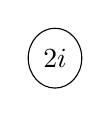
\begin{tikzpicture}\draw (0,0) ellipse (.34 and .38);\node at (0,0) {$2i$};\end{tikzpicture}}}
Par exemple, on définit le \uline{bicristal de Tate de poids \inserted{2}i}, qui est défini par le cristal de modules unité (associant à tout T sous S le Module $\underline O_T$ lui-même), et les \deleted{\unsure{appliqu}} morphismes de cristaux
\[
F=p^i\operatorname{id}_{T^i},\qquad V=p^i\operatorname{id}_{T^i}.
\]
Ainsi le bicristal de Tate de poids 2i est la puissance tensorielle i.ème du bicristal de Tate de poids 1. (NB les bicristaux de poids quelconques se multiplient tensoriellement, de \deleted{sorte} \inserted{\unsure{façon}} que les poids s'ajoutent).

1.11. Si on veut ``rendre inversible'' le bicristal de Tate $T^1$, on est obligé, qu'on le veuille ou non, de passer à une catégorie de fractions de la catégorie des cristaux de modules sur S, \inserted{[}qui entre parenthèses est une catégorie $\underline Z_p$-linéaire, (i.e. les Hom sont des $\underline Z_p$-modules ...), tout comme les catégories de p-cristaux etc qu'on en déduit\inserted{]}. Il revient donc au même de passer à une catégorie de fractions, en déclarant qu'on veut rendre notre catégorie abélienne $\underline Q$-linéaire, ou en déclarant qu'on la veut rendre $\underline Q_p$-linéaire: il faut faire le quotient par la sous-catégorie abélienne épaisse formée des objets de \deleted{p-}\unsure{torsion}, qui sont aussi des objets de p-\unsure{torsion}\inserted{\figure{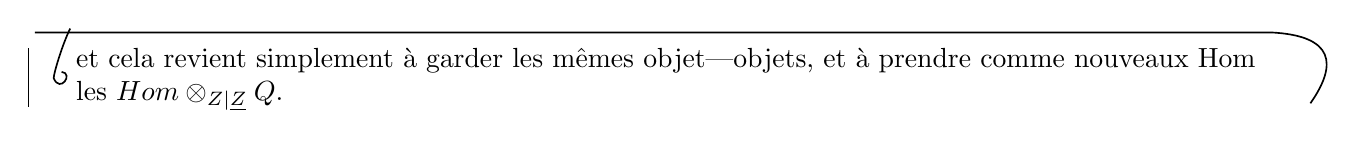
\begin{tikzpicture}
\draw[line width=.6pt] (0,0)--(15.7,0) .. controls (16.5,-.04) and (16.55,-.4) .. (16.2,-.9);
\draw[line width=.6pt] (-.08,-.2)--(-.08,-.95);
\draw[line width=.6pt] (.45,.05) .. controls (.35,-.15) and (.24,-.52) .. (.24,-.58) .. controls (.32,-.78) and (.5,-.52) .. (.34,-.5);
\node[anchor=north west,text width=15.2cm,align=left] at (.4,-.08) {et cela revient simplement à garder les mêmes \unsure{objet|objets}, et à prendre comme nouveaux Hom les $\operatorname{Hom}\otimes_{\unsure{Z|\underline Z}}Q$.};
\end{tikzpicture}}}. On trouve la catégorie des ``\uline{cristaux de modules}
\margin{8}


\scanpage{10}
\mspage{8}

\uline{à isogénie près}'', ou \uline{isogristaux}, sur S. Utilisant cette nouvelle notion, on définit comme ci-dessus la notion de p-isocristal, comme étant la donnée d'un isocristal $\underline M$ muni d'un homomorphisme $F:\underline M^{(p)}\longrightarrow\underline M$. La notion de bi-isocristal de poids i, qui serait calquée de celle de bi-cristal de poids i, n'est pas très raisonnable alors, car V doit être alors donné en termes de F comme $p^{\deleted{\unsure{2}}i}F^{-1}$. Il y a lieu plutôt d'appeler \uline{bi-isocristal} (sans précision de poids) un p-isocristal pour lequel F est un \uline{isomorphisme}, et de ne pas choisir entre les différents $p^{\deleted{\unsure{2}}i}F^{-1}$ possibles; il vaut mieux également ne pas parler ici de $p^{-1}$-isocristal, la notion intéressante étant celle de bi-isocristal, qui est manifestement \uline{autoduale} \deleted{(si $\unsure{\phi|F}$ est un foncteur contravariant de catégories fibrées sur un} \inserted{quand on se restreint aux objets de type fini:} le dual de $(\underline M,F)$ est $(\underline M,{}^tF^{-1})$, où $\underline M$ est le iso-cristal dual de M.

On peut également, bien sûr, localiser par rapport à p en partant déjà de la catégorie des bi-cristaux de poids i, on trouve les \uline{bicristaux de poids} i \uline{à isogénie près}, qui forment une catégorie abélienne $\mathrm{Is}\inserted{\mathrm{bi}}\mathrm{cr}(S,i)$, et un foncteur exact ``oubli de V''
\[
\unsure{\operatorname{Isbicr}|\operatorname{IsBicr}}(\unsure{S,i|S)i})\longrightarrow\operatorname{Isbicr}(S),
\]
à valeurs dans la catégorie $\operatorname{Isbicr}(S)$ des iso-bi-cristaux sur S. Ce foncteur est \deleted{\unsure{évidemment}} \uline{pleinement fidèle}, de sorte que \uline{les \inserted{\unsure{iso-}}bicristaux forment une généralisation commune des bicristaux de poids} i \uline{à isogénie près}. Pour préciser ce point, désignant par $\operatorname{Bicr}(S,i)$ la catégorie des bicristaux de poids i sur S, il y a lieu d'introduire des foncteurs canoniques
\[
\operatorname{Bicr}(S,i)\longrightarrow\operatorname{Bicr}(S,i+1)\longrightarrow\ldots,
\]
donnés par $(\underline M,F,V)\rightsquigarrow(\underline M,F,pV)$. Quand on localise ces foncteurs par p, on trouve des foncteurs
\[
\operatorname{IsBicr}(S,i)\longrightarrow\operatorname{IsBicr}(S,i+1)\longrightarrow\ldots.
\]
qui se trouvent être \uline{pleinement fidèles} : on peut donc considérer que, pour i croissant, la notion de ``bicristal de poids i, à isogénie près'' constitue une généralisation de plus en plus large de celle de ``cristal de Dieudonné''. La noti-
\margin{9}


\scanpage{11}
\mspage{9}

de ``bi-isocristal'' est à ce titre une \deleted{globalisation} \inserted{généralisation} qui englobe toutes les précédentes, et qui de plus a la louable vertu d'être stable par produit tensoriel\unsure{,|.} \inserted{et passage au dual.} Cela semble donc une catégorie toute indiquée \deleted{pour recevoir} comme catégorie des valeurs pour un foncteur ``cohomologie de De Rham'' convenable, lorsqu'on se décide à travailler à isogénie près.

1.12. \deleted{\unsure{Isocri|Isocr}} \uline{Exemple} \inserted{1}: \uline{Cas où} S \uline{est le spectre d'un corps parfait} k. Alors la donnée d'un cristal de modules de type fini sur k équivaut à la donnée d'un module de type fini M sur W, la formation du motif $\underline M^{(p)}$ correspond à la formation de
\[
M^{(p)}=M\otimes_W(W,f_W),
\]
où $f_W$ est l'endomorphisme de frobenius de W, \deleted{qui} et $(W,f_W)$ est la W-algèbre dé\unsure{fi}nie par $f_W$. Par suite un structure de p-cristal sur M revient à la donnée d'un homomorphisme de W-modules $M^{(p)}\longrightarrow M$, ou si on préfère, à la donnée d'un homomorphisme $f_W$\deleted{\unsure{,|-}} semi-linéaire
\[
F_M:M\longrightarrow M.
\]
Comme l'application $x\rightsquigarrow x\otimes1$ de M dans $M\otimes_W(W,f_W)$ est bijective, $f_W$ étant un automorphisme de W, on peut considérer la bijection inverse, qui est $f_W^{-1}$-semi-linéaire. Par suite, la donnée d'une $p^{-1}$-structure sur M revient à la donnée d'un homo\unsure{morphisme|morpbisme} $f_W^{-1}$-linéaire:
\[
V_{\inserted{M}}:M\deleted{\unsure{T}}\longrightarrow M.
\]
la donnée d'un couple $(F,V)$ définit sur M une structure de bi-cristal de poids i si et seulement si on a
\[
FV=VF=p^i\operatorname{id}_M.
\]
En particulier, pour $i=1$, on retrouve la notion de \uline{module de Dieudonné}: la catégorie des cristaux de Dieudonné sur k est canoniquement équivalente à celle des modules de Dieudonné \deleted{sur k} relativement à k.

La catégorie des isocristaux de \deleted{modules} type fini sur k est équivalente à la catégorie des vectoriels de dimension finie sur le corps des fractions \inserted{K}\deleted{$\unsure{W\otimes\underline Q_p|W_{\underline Q_p}}$} de W. Donc un bi\inserted{iso}cristal (de type fini) sur k s'identifie à un tel vectoriel, muni d'un $f_K^{\deleted{\unsure{-1}}}$-endomorphisme bijectif.
\margin{10}


\scanpage{12}
\mspage{10}

Toutes ces d\unsure{es}criptions sont compatibles avec les opérations tensorielles, et la formation d'images inverses pour k variable.

On peut se demander, avec la description précédente des bi-isocristaux, quels sont ceux qui sont dans l'image essentielle de $\unsure{\operatorname{Isbicr}|\operatorname{Hsbicr}}(S,i)\longrightarrow\operatorname{Isbicr}(S)$. On trouve que ce sont les couples $(E,F)$, E un vectoriel sur K et F un automorphisme semi-li\unsure{né}aire, tels que, si on pose $V=p^iF^{-1}$, pour tout $x\in E$, l'ensemble de ses transformés par les différents monômes non commutatifs en F,V soit une partie \uline{bornée} de E: c'est une pure tautologie. Pour qu'il existe un i ayant cette propriété, il faut et il suffit que pour tout $x\in E$, l'ensemble des $F^nx$ soit borné. Bien entendu, c'est là une propriété qui est stable par changement de F en pF (correspondant à la tensorisation par le bi-isocristal de Tate de poids 2), mais non par le changement de F en $p^{-1}F$ (correspondant à la tensorisa\unsure{tion|gion} par l'inverse $T^{-1}$ du bi-isocristal précédent). Comme on tient beaucoup à inverser Tate, on voit qu'il n'est pas naturel, en effet, de poser une condition de croissance sur l'ensemble des \deleted{\unsure{iétér|itér}} itérés de F. De façon précise, appelant \uline{effectifs} les bi-\unsure{is}ocristaux qui proviennent d'un objet d'un $\operatorname{Isbicr}(S,i)$, on voit que tout bi-isocristal est de la forme $T^{-i}\otimes\underline N$, avec $\underline N$ effectif: on n'a pas ajouté plus de nouveaux objets qu'il n'était absolument nécessaire !

1.13. \uline{Exemple} 2: S \uline{lisse sur un corps parfait} k. Déterminons d'abord dans ce cas les cristaux sur S, sans plus. \unsure{Tout|Wout} d'abord, sans condition de lissité, on voit à l'aide de la propriété caractéristique de W que la catégorie C introduite dans 1.0. ne change pas, essentiellement, quand on remplace $R=\operatorname{Spec}(\underline Z)$ par $R=\operatorname{Spec}(W)$. D'autre part, il résulte aussitôt des définitions que la donnée d'un \deleted{\unsure{R-}}cristal sur S, relativement à R, revient à la donnée d'un système cohérent de cristaux sur S, relatifs aux $W_n=W/p^{n+1}W$. (NB On n'a pas formulé avec la généralité qui convenait l'exemple 3 de 1.7. ! ) Théoriquement, on est donc ramené à déterminer, pour chaque n, la catégorie des cristaux sur S relatifs à $W_n$, et les foncteurs restriction entre ces catégories. D'ailleurs, il est inoffensif de se localiser sur S, \deleted{\unsure{Ceci|aussi}} par exemple de supposer au besoin S affine. Utilisant maintenant la lissité de S, on peut donc supposer que pour tout n, S se remonte en
\margin{11}


\scanpage{13}
\mspage{11}

un $S_n$ lisse sur $W_n$, de façon que ces choix se recollent (il suffit pour ceci S lisse et affine). Or, il résulte encore facilement des définitions, utilisant seulement que $S=S_0\longrightarrow S_n$ est une immersion fermée définie par un Idéal nilpotent, que le foncteur restriction des cristaux sur $S_n$ (relativement à une base quelconque -- ici on prendra $\unsure{R_n|W_n}$) vers les cristaux sur $S_0$, est une équivalence de catégories, donc un cristal sur S relativement à $\unsure{R_n|W_n}$ s'identifie à un cristal \inserted{sur $S_n$} relativement à $\unsure{R_n|W_n}$. Comme $S_n$ b est lisse sur $W_n$, il résulte de ce qui a été dit dans 1.8. que les cristaux en question s'identifient aux objets (de l'\unsure{espàce|espèce} $\underline F$ considérée) sur $S_n$, \uline{munis d'une stratification relativement à} $R_n=\operatorname{Spec}(W_n)$. Les foncteurs restrictions sur les cristaux s'expriment alors par les foncteurs restrictions correspondants pour objets stratifiés. En résumé: \uline{un cristal} \inserted{$\underline M$} \uline{sur} S \uline{s'identifie à un} \deleted{\unsure{pour|Pour}} \uline{système cohérent} $(\underline M_n)$ \uline{d'objets à stratification sur les différents} $S_n$ \uline{sur} $R_n=\operatorname{Spec}(W_n)$. Pour relier ceci à des objets qui soient plus dans la nature d'objets ``définis en caractéristique nulle'', supposons d'abord\unsure{s} que l'on puisse même relever S en un schéma X \uline{propre sur} $R=\operatorname{Spec}(W)$, hypothèse évidemment bien restrictive. On voit alors, utilisant les théorèmes de comparaison EGA III 4,5 que \uline{dans le cas de cristaux de modules dohérents sur} S, \uline{la catégorie desdits est canoniquement équivalente à la catégorie des Modules cohérents} $\underline M$ \uline{sur} X, \uline{munis d'une stratification relativement à} $R=\operatorname{Spec}(W)$. (NB Il se trouve donc, à posteriori, que cette \unsure{dernière|detnière} catégorie est essentiellement indépendante du relèvement choisi X de S). Considérant la fibre générique $X_K$ \deleted{sur} de X sur R, qui est un schéma propre et lisse sur un corps de caractéristique nulle, \unsure{on|oj} trouve donc un foncteur remarquable ``restriction'' ou ``localisation'', allant de la catégorie des cristaux de modules cohérents sur S, dans la catégorie des Modules cohérents \deleted{stratifiés} sur $X_K$, stratifiés relativement à $X_K$. Or (oubli de 1.8.) on voit \unsure{facilement} qu'un Module cohérent stratifié sur un préschéma localement de type fini sur un corps est nécessairement localement libre. De plus comme ici K est de caractéristique nulle \inserted{et $X_K$ lisse dessus}, on a signalé dans 1.8. que la notion de stratification s'explicite très simplement comme celle de ``connexion inté-
\margin{12}


\scanpage{14}
\mspage{12}

grable''. \inserted{[}Enfin, lorsque S donc $X_K$ est géométriquement connexe, et que K peut se plonger dans le corps des complexes $\underline C$, alors la notion de module cohérent à \unsure{conn|comn}\inserted{ex}ion intégrable sur $X_K$ s'interprète en termes de représentations linéaires \inserted{(complexes)} du groupe fondamental \deleted{\unsure{du|de}} transcendant de $X_{\underline C}^{\mathrm{an}}$, de façon bien connue. Si par exemple le groupe fondamental transcendant est le groupe unité, alors on conclut par descente que tout Module cohérent stratifié sur $X_K$ est trivial, ce qui en termes de S s'énonce en disant que tout cristal de modules cohérents sur S est isogène à un cristal ``con\unsure{st|ss}ant'', i.e. \deleted{image} \inserted{à un cristal} qui est l'image inverse d'un cristal sur k, (lui-même défini par un module de type fini sur W). De ceci et de la rigidité de la notion de cristal on déduit\figure{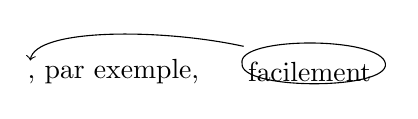
\begin{tikzpicture}[baseline=(p.base)]
\node[anchor=west,inner sep=0] (p) at (0,0) {, par exemple,};
\node[anchor=west,inner sep=0] (f) at (2.8,0) {facilement};
\draw (2.73,0.1) .. controls (2.65,0.45) and (4.5,0.45) .. (4.55,0.1) .. controls (4.6,-0.24) and (2.7,-0.24) .. (2.73,0.1);
\draw[->] (2.75,0.32) .. controls (1.7,0.55) and (0.1,0.55) .. (0.04,0.14);
\end{tikzpicture}} que tout p-cristal cohérent sur S ou tout bi-cristal de poids i donné (par exemple tout cristal de Dieudonné) \deleted{sur S} est isogène à un fourbi\deleted{\unsure{s}} de même espèce \uline{trivial}. On voit donc là un principe d'approche transcendante pour l'étude des familles de groupes formels (par exemple) en caractéristique p \ldots\inserted{]}

Quand à la notion d'isocristal (de modules cohérents) sur S, on constate aussitôt que le foncteur précédent induit un foncteur \uline{pleinement fidèle} de la catégorie de ces derniers, dans la catégorie des modules cohérents stratifiés sur $X_K$. Il s'impose évidemment d'en déterminer l'image essentielle, et pour commencer d'examiner \deleted{\unsure{préliminairement}} si par hasard ce foncteur ne serait pas une équivalence de catégories. \deleted{\unsure{(}}Cela me semble un peu $\underset{\sim\ \sim\ \sim}{\text{trop optimiste}}$, mais je ne suis sûr de rien, faute d'avoir regardé.
\margin{effectivement, ça \unsure{ne} marche pas !}
Tout ce qu'on peut dire à priori, c'est que la condition cherchée sur un\deleted{e} Module stratifié doit être\deleted{, à priori} de nature locale en les points de X qui sont maximaux dans S.

Quand on ne suppose pas S \deleted{remonté} propre\deleted{ment} et remonté globalement, mais qu'on suppose seulement qu'on a remonté S formellement, en un \uline{schéma formel} X sur \unsure{R|B}, alors il est vrai (en fait, de façon essentiellement triviale) que \uline{la catégorie des cristaux} \deleted{sur} \uline{de modules cohérents sur} S \uline{est équivalente à la catégorie des Modules cohérents sur le schéma formel} X, \uline{munis d'une stratification relativement à} $\operatorname{Specf}(W)\inserted{=R}$ (quand on transcrit de façon évidente toutes les définitions envisagées dans 1.8. dans le cadre formel). Si on veut encore,
\margin{13}


\scanpage{15}
\mspage{13}
comme il est légitime, trouver un analogue \deleted{pour} \inserted{\unsure{de}} la restriction à $X_K$ \inserted{\unsure{envisagée|envisagé}} plus haut, il faut définir $X_K$ comme \uline{l'espace rigide-analytique sur $K$ défini par le schéma formel} $X$, et considérer sur $X_K$ des Modules cohérents munis de \deleted{connexions} \uline{stratifications au sens rigide-analytique}, ou ce qui revient au même, de connexions intégrables \inserted{en ce sens}. De tels Modules sont encore nécessairement localement libres. On trouve ainsi un foncteur des cristaux de Modules cohérents sur $S$ dans les Modules cohérents stratifiés sur $X_K$, induisant un foncteur pleinement fidèle de la catégorie des isocristaux cohérents sur $S$, dans la catégorie des Modules cohérents stratifiés sur $X_K$. Comme tout à l'heure (et même plus, si on peut dire, car c'est vraiment \deleted{\unsure{si|ici}} ici la situation ``naturelle''), il s'impose de regarder quelle est l'image essentielle. On peut également se demander si les Modules cohérents stratifiés sur un espace rigide-analytique n'admettraient pas une description simple, en termes d'un groupe plus ou moins discret jouant le rôle du groupe fondamental dans la théorie transcendante sur le corps des complexes.

\deleted{\unsure{1.14.}} La description donnée \inserted{des cristaux sur $S$}, toute triviale qu'elle soit, a déjà des conséquences intéressantes pour la structure de la catégorie des cristaux \inserted{de modules} cohérents sur $S$: \deleted{\unsure{un tel cristal}} cette catégorie est noethérienne (si $S$ est noethérien i.e. de type fini sur $k$), tout objet contient donc un plus grand sous-objet de torsion, de plus \deleted{\unsure{un}} \inserted{les} objets sans torsion correspond\inserted{ent} dans la description ci-dessus \deleted{\unsure{à un}} \inserted{aux} Modules stratifiés sans torsion sur $X$, lesquels \deleted{\unsure{est}} \inserted{sont} alors automatiquement localement libres. Il est bien probable que des résultats analogues doivent être vrais, sans hypothèse du genre lissité sur $S$.

1.14. Il faut encore expliciter, dans la description générale précédente, la \deleted{donnée} foncteur $M\rightsquigarrow M^{(p)}$, pour pouvoir décrire de façon analogue les bicristaux et bi-isocristaux. De façon générale, si en plus de la donnée de $S$ sur $k$, on a un $S'$ lisse sur $k'$ parfait, et des \deleted{\unsure{homo}}morphismes $S'\longrightarrow S$ et $\operatorname{Spec}(k')\longrightarrow\operatorname{Spec}(k)$ donnant lieu à un carré commutatif, et si enfin on peut relever $S'$ formellement en $X'$, et $S'\longrightarrow S$ en $X'\longrightarrow X$, donnant un carré commutatif avec $\operatorname{Spec}W'\longrightarrow\operatorname{Spec}W$, alors la notion d'image inverse de cristaux de modules cohérents, de $S$ à $S'$, s'explicite en termes d'image inverse de Modules cohérents stratifiés, de $X$
\margin{14}


\scanpage{16}
\mspage{14}
à $X'$. Lorsque $k=k'$, $S=S'$, et que les morphismes envisagés sont les puissances $p$.èmes, on est donc conduit à chercher à \deleted{prolonger} relever ce morphisme à $X$ de façon compatible avec le morphisme $\operatorname{Specf}(W)\longrightarrow\operatorname{Specf}(W)$ déduit de $f_W$, ou ce qui revient au même, de relever le morphisme canonique $S\longrightarrow S^{(p/k)}$ en un morphisme de $R$-schémas formels $X\longrightarrow X\times_R(R,f_R)$. C'est en tous cas toujours possible si $S$ est affine, cas auquel on peut se ramener. Ayant donc ainsi un morphisme
\[
f_X:X\longrightarrow X,
\]
compatible avec $f_R$ sur $R=\operatorname{Specf}(W)$, et induisant $f_S$ sur $S$, le foncteur $\underline{M}\rightsquigarrow\underline{M}^{(p)}$ s'explicite comme l'image inverse ordinaire de Modules stratifiés sur $X$ relativement à $R$, resp. (dans le cas de isocristaux) de Modules stratifiés sur l'espace rigide-analytique $X_K$, pour le ``morphisme'' $X_K\longrightarrow X_K$ d'espaces rigide-analytiques (relatif à $f_K$ sur le corps de base !) induit par $f_X$. Bien que $f_X$ et par suite $f_{X_K}$ \unsure{soit} loin d'être unique, le foncteur envisagé qu'il définit ne dépend pas, essentiellement, des choix faits.

1.15. \uline{Bicristaux et biisocristaux sur une base quelconque}. Ne supposons plus nécessairement $S$ de caractéristique déterminée $p$. \deleted{Nous} Pour chaque nombre premier $p$, soit $S_p$ la fibre $V(p.1_{\underline{O}_S})$ de $S$ sur le point $p\underline{Z}$ de $\operatorname{Spec}(\underline{Z})$. Un bicristal de poids $i$ sur $S$ est par définition la donnée d'un cristal de modules $\underline{M}$ sur $S$, et pour chaque $p$ d'une structure de bi-cristal de poids $i$ sur la restriction $\underline{M}_p$ de $\underline{M}$ à $S_p$, définie par la donnée de $F_p,V_p$. On définit de même la notion de bi-isocristal sur $S$, étant entendu qu'un isocristal est un objet de la catégorie des isocristaux sur $S$ (comme de juste), définie à partir de la catégorie des cristaux de modules en ``localisant'' par rapport à des entiers $n>0$ arbitraires, i.e. en tensorisant les $\operatorname{Hom}$ sur $\underline{Z}$ par $\underline{Q}$. - Lorsque $S$ est de caractéristique nulle, le supplément de structure impliqué par ``bi'' est évidemment vide, tandis que si $S$ est de caractéristique $p$, on retrouve les notions de 1.10. Lorsque enfin $S$ est de type fini sur $\underline{Z}$ et domine $\operatorname{Spec}(\underline{Z})$, alors la notion envisagée est d'une nature essentiellement arithmétique, les différents $F_p$ jouant le rôle d'homomorphismes de frobenius, comme de bien entendu; dans le cas du poids 1, en
\margin{15}


\scanpage{17}
\mspage{15}
particulier, on peut considérer que le cristal avec sa bi-structure supplémentaire permet de relier entre eux les groupes formels en les diverses caractéristiques auxquels il donne naissance $\ldots$

1.16. \uline{Un retour en arrière}. La définition 1.1. et le sorite 1.3. sont un petit peu canulés. Au lieu de prendre dans 1.0. pour $C$ la catégorie des \inserted{$R$-}flèches $S\longrightarrow T$ qui $\ldots$, il faut prendre la catégorie des $R$-flèches $U\longrightarrow T$ qui $\ldots$, où $U$ est un ouvert induit non précisé de $S$. De plus, \deleted{\unsure{il}} la définition n'est guère raisonnable alors que si la catégorie fibrée envisagée $\underline{F}$ est un ``champ'' pour la topologie de Zariski sur $(\operatorname{Sch})_{/R}$, i.e. si on peut y recoller flèches et objets. Ceci est nécessaire en tous cas pour pouvoir dans 1.3. définir la notion d'image inverse, la définition que j'y ai donnée n'étant raisonnable que si $S,S'$ sont affines. Dans le cas général, il faut se localiser sur $S$ et $S'$ pour se ramener à cette situation. Autrement on bute sur des canulars idiots de nature globale, comme le fait que sans restriction sur $S'\to S$, la construction \deleted{indiquée} \inserted{envisagée} de somme amalgamée fait sortir de la catégorie des préschémas $\ldots$ Il est probable qu'il y aura bien d'autres canulars de détail dans ces notes, mais, je pense, sans conséquence !

Il est évidemment tentant de vouloir interpréter les cristaux de modules comme faisceaux de modules sur un certain site. C'est possible, en prenant le ``\uline{site cristallogène} \uline{de} $S$ \uline{sur} $R$'', qui est précisément le site dont la catégorie sous-jacente \inserted{$C$} est celle des $R$-morphismes $U\longrightarrow T$ ($U$ ouvert de $S$, $U\longrightarrow T$ immersion fermée surjective définie par Ideal nilpotent sur $T$), la topologie est celle de Zariski: on prend comme familles couvrantes ``de définition'' de $(U\longrightarrow T)$ les familles définies par des recouvrements ouverts $(T_i)$ de $T$, chaque $T_i$ muni de la structure induite, et définissant $(U_i\longrightarrow T_i)$ par $U_i=U\cap T_i$. Un faisceau d'ensembles sur ce site s'identifie à un système de faisceaux d'ensembles $F_{U\to T}$ sur les \inserted{objets} buts des objets de $C$, avec, pour toute flèche $(U\longrightarrow T)\longrightarrow(U'\longrightarrow T')$ de $C$, un homomorphisme de l'image inverse de $F_{U'\to T'}$ \deleted{sur} \deleted{dans} \inserted{sur} $T$, dans $F_{U\to T}$ (homomorphisme qui n'est pas nécessairement un isomorphisme !)\inserted{(et qui est un \unsure{isom} si $T\unsure{\longrightarrow|-}T'$ est une \unsure{imm. ouverte})}. En particulier, associ-
\margin{16}


\scanpage{18}
\mspage{16}
ant \deleted{en particulier} à tout $(U\to T)$ le faisceau $\underline{O}_T$ sur $T$, on trouve un faisceau d'anneaux $\underline{O}_C$ sur $C$. Ceci posé, les cristaux de modules (quasi-cohérents) sur $S$ s'identifient aux Modules quasi-cohérents (i.e. localement conoyau d'un homomorphisme de Modules libres) sur $\underline{O}_C$; les cristaux ``de \deleted{type} \inserted{prés.} finie'' i.e. les cristaux de Modules de présentation finie, correspondent exactement aux Modules de présentation finie sur $\underline{O}_C$.

Quand on a un $R$-morphisme $S'\longrightarrow S$, je ne vois pas de morphisme naturel correspondant entre les \uline{sites} cristallogènes correspondants à $S,S'$. Ce n'est pas bien gênant, car introduisant les \uline{topos cristallogènes} \inserted{$\operatorname{Topcr}_{S/R}$ et $\operatorname{Topcr}_{S'/R}$} définis par les sites en question, on définit par la méthode esquissée dans 1.3. un \deleted{homo}morphisme
\[
\operatorname{Topcr}_{S'/R}\longrightarrow\operatorname{Topcr}_{S/R},
\]
correspondant à la notion naturelle de ``image inverse de faisceaux'' \inserted{en sens inverse} (qui, j'avoue, devrait être définie avec le plus grand soin).

1.17. On est donc dans une situation où on peut faire marcher la machine cohomologique. Etant loin de mes bases, je n'ai pas tenté sérieusement de tirer au clair si les images directes supérieures qu'on définit ainsi, et en particulier les groupes de cohomologie du site cristallog\deleted{\unsure{raphique}}\inserted{ène}, donnent ce qu'on voudrait. Le test-clef est le suivant: \uline{si} $R$ \uline{est le spectre d'un corps}, \uline{et si} $S$ \uline{est lisse sur} $R$, \uline{et propre sur} $R$ \uline{dans le cas de la caractéristique} $p>0$, \uline{on voudrait trouver}, \uline{comme cohomologie à coefficients dans} $\underline{O}_C$ \uline{lui-même}, \uline{la cohomologie de De Rham de} $S$ \uline{relativement à} $R$.
\margin{\uline{marche en car. $0$, et \uuline{pas} en car $p>0$} (\unsure{faut|faute} d'introduire \unsure{les} puiss. div.)}
Plus généralement, sans condition sur $R$, si $f:S'\to S$ est propre et lisse, on voudrait trouver comme \inserted{``valeur en $S'$'' de} $R^if_{\mathrm{cris}\,*}(\underline{O}_{C'})$ \inserted{(cf 1.4)} le faisceau de cohomologie de De Rham $\underline{R}^if_*(\underline{\Omega}^{*}_{S'/S})$, \deleted{\unsure{et et comme connexion}} et \inserted{on voudrait} que la connexion canonique à la Gauss-Manin sur ce dernier soit celle associée à la stratification canonique provenant de la structure cristalline (cf 1.8.). L'existence d'une connexion de Gauss-Manin en cohomologie de De-Rham (que j'ai vérifié pour n'importe quel morphisme lisse), et le tapis de Washnitzer-Monsky, sont en tous cas des indications assez fortes pour conduire à penser qu'il doive exister une théorie cohomologique, en termes de cristaux, donnant de telles valeurs pour l'argument $\underline{O}_C$. Au cas où la cohomologie du site cris-
\margin{17}


\scanpage{19}
\mspage{17}
tallogène ne donnerait pas les résultats qu'il faut, on pourrait ess\inserted{a}yer (au lieu de prendre des foncteurs dérivés dans la catégorie de \uline{tous} les Modules sur le site annelé cristallog\deleted{\unsure{raphique}}\inserted{ène}) de prendre des foncteurs dérivés dans la catégorie des seuls Modules quasi-cohérents sur le site cristallogène, i.e. dans la catégorie des cristaux de modules. \unsure{?}

\uline{Chapitre} 2 \uline{La cohomologie de De Rham est un cristal}.

2.1. L'affirmation du titre n'est pour l'instant qu'une hypothèse ou un voeux pieux, mais je suis convaincu qu'elle est essentiellement correcte. Comme je l'ai dit dans 1.17., il y a pour le moment deux indications dans cette direction:

a) Le travail de Washnitzer-Monsky. Deux grosses imperfections dans leur tapis: $1^{\mathrm{o}}$ ils n'obtiennent que des invariants cohomologiques \uline{locaux} sur leur variété lisse en caractéristique $p>0$, via leurs relèvements; pour avoir un invariant global, ils doivent se limiter à la dimension 1. On peut penser que cela tient à leur manque de familiarité avec les machines cohomologiques. $2^{\mathrm{o}}$ leurs invariants sont des (faisceaux de) vectoriels sur le corps des fractions de $W$, et non sur $W$, i.e. ils n'obtiennent que des invariants ``modulo isogénie''. Il semble bien, en effet, que leur démonstration d'invariance fait intervenir de façon \deleted{ass} essentielle des dénominateurs. Il n'est pas exclu, d'après cette indication, que dans le titre du Chapitre il faille remplacer ``cristal'' par ``isocristal''\inserted{(et ``est'' par ``définit'')}. Ce serait bien dommage, mais n'exclurait pas pour autant l'existence d'une bonne théorie cohomologique pour les cristaux, qui pour un morphisme propre et lisse et le ``cristal unité'' coïnciderait \uline{modulo isogénie} avec ce que donne De Rham. Le test décisif reste celui indiqué dans 1.17, savoir: donne-t-il un résultat positif seulement en caractéristique zéro, ou en toute caractéristique ?

b) L'existence des connexions de Gauss-Manin. \deleted{Comme} J'ai vérifié pour tout morphisme lisse $f:\deleted{\unsure{S'}}\inserted{X}\longrightarrow S$ l'existence d'une connexion canonique \inserted{(absolue)} sur les $\underline{R}^if_*$ au sens de De Rham relatif, ou plus correctement, sur le complexe
\margin{18}


\scanpage{20}
\mspage{18}
$\underline{R}f_*(\underline{\Omega}^{\bullet}_{X/S})$, considéré comme objet de la catégorie dérivée $D(\underline{O}_S)$. A vrai dire, je n'ai pas vérifié pour cette connexion une condition de ``nullité de la \deleted{\unsure{torsion}} \inserted{courbure}''; c'est \deleted{vrai} vérifié en tous cas (par voie transcendante !) si $S$ est lisse, sur $R$ réduit de caractéristique nulle. [Il faut noter d'ailleurs qu'il n'y a pas d'espoir de montrer que la connexion en question provient toujours d'une stratification: c'est \uline{faux} en caractéristique $p>0$; la raison étant que la cohomologie de De Rham pour une variété algébrique non complète (par exemple affine) n'est plus du tout raisonnable, étant beaucoup trop grosse. Pour pouvoir espérer une stratification sur $\underline{R}f_*(\underline{\Omega}^{\bullet}_{X/S})$, sans restriction de caractéristique, il faut donc supposer $f$ \uline{propre}.]

c) La nécessité d'une interprétation cristallographique de la cohomologie de De Rham est également suggérée par le problème que j'avais signalé dans mon papier bleu sur De Rham: si $R$ est le spectre du corps des complexes, $S$ lisse sur $R$ et $X$ lisse et propre sur $S$, alors la théorie transcendante de la cohomologie nous fournit une suite spectrale $H^p(S^{\mathrm{an}},R^qf^{\mathrm{an}}_*(\underline{C}_{S^{\mathrm{an}}}))\Longrightarrow H^{\bullet}(X^{\mathrm{an}},\underline{C})$, dont le terme initial et l'aboutissement d'autre part ont une description purement algébrique, comme cohomologie de De Rham de $X$, et de $S$ à coefficients dans les $\underline{R}^qf_*(\underline{\Omega}^{\bullet}_{X/S})$ \uline{munis de leur connexion canonique} \inserted{\uline{intégrable}} (ce qui permet de les prendre comme coefficients dans la cohomologie de De Rham). On aimerait trouver une interprétation purement algébrique de cette suite spectrale toute entière.

2.2. Je vais préciser \deleted{\unsure{un genre d'énoncé précis}} l'affirmation du titre, en me plaçant \figure{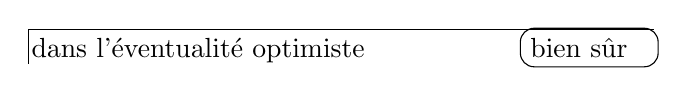
\begin{tikzpicture}[baseline=(a.base)]
\node[anchor=base west,inner sep=1pt] (a) at (0,0) {dans l'éventualité optimiste};
\node[anchor=base west,inner sep=2pt] (b) at (6.3,0) {bien sûr};
\draw (0,-0.08)--(0,0.35)--(7.95,0.35);
\draw[rounded corners=5pt] (6.25,-0.12) rectangle (8,0.37);
\end{tikzpicture}} où on n'aurait pas besoin de s'isogéniser.
\deleted{On \deleted{veut} désigne, pour abréger, par le mot ``\uline{complexe}'' \unsure{sur} un préschéma $S$, un complexe de Modules à cohomologie quasi-cohérente, considéré comme objet de la catégorie dérivée qu'on sait; Les catégories de ces complexes, pour une base variable,}
Comme les cristaux de modules sur un préschéma $S$ forment une catégorie abélienne, on peut prendre la catégorie dérivée; ses objets seront appelés simplement ``complexes de cristaux''. Un tel animal induit sur $S$, et plus généralement sur tout objet-but $T$ d'un objet $(U\longrightarrow T)$ du site cristal-
\margin{19}


\scanpage{21}
\mspage{19}
logène \inserted{$C$} de $S$, un complexe de Modules ordinaire (envisagé comme objet de la catégorie dérivée des faisceaux de Modules sur $S$, resp. $T$). Un complexe de cristaux est dit pseudo-cohérent (resp. parfait, resp. $\ldots$) si pour tout objet $(U\to T)$ de $C$, le complexe induit sur $T$ est pseudo-cohérent (resp. $\ldots$). Ceci posé, voilà la théorie qu'on voudrait: A tout morphisme lisse et propre $f:X\to S$, serait associé un complexe de cristaux \inserted{(absolu)} $\operatorname{DR}(f)$ \inserted{sur $S$}, appelé cohomologie de De Rham \inserted{cristalline} de $f$. \margin{\unsure{c}} Ce complexe doit être parfait, sa formation doit être compatible avec tout changement de base sur $S$ (l'image inverse des complexes de cristaux étant entendue, bien entendu, au sens de catégories dérivées $\ldots$), et bien sûr $\operatorname{DR}(f)$ dépend fonctoriellement (de façon cotravariante) de $X$ sur $S$. Tôt ou tard, il faudra expliciter aussi une formule de Künneth $\operatorname{DR}(f\times_Sg)\simeq\operatorname{DR}(f)\overset{L}{\otimes}\operatorname{DR}(g)$, et une formule de dualité, qui pour $f$ partout de dimension relative $d$ s'exprime comme un accouplement, définissant une autodualité, $\operatorname{DR}(f)\times\operatorname{DR}(f)\longrightarrow T^d[2d]$, où $T^d$ est le cristal de Tate de poids $2d$, et où $[2d]$ indique qu'on translate les degrés de $2d$ (attention au facteur 2 !). Enfin, on veut comme de juste un isomorphisme $\operatorname{DR}(f)(S)\simeq\underline{R}f_*(\underline{\Omega}^{\bullet}_{X/S})$, fonctoriel en $X$, compatible avec les changements de base, avec Künneth et la dualité (déjà connus pour la cohomologie de De Rham ordinaire).

Par prudence, je me suis abstenu de dire quoi que ce soit sur le cas $f$ non propre, dont il faudrait parler tout au moins si on voulait faire sérieusement le lien avec Washnitzer-Monsky.

2.3. \uline{La cohomologie de De Rham comme bi\inserted{iso}cristal}. A supposer qu'on ait une théorie du type envisagé dans 2.2., \deleted{on constate aussitôt que chaque} on trouve pour chaque entier $p$ un homomorphisme de frobenius
\[
F_p:\operatorname{DR}(f)_p^{(p)}\longrightarrow\operatorname{DR}(f)_p,
\]
où l'indice $p$ au complexe de cristaux $\operatorname{DR}(f)$ désigne la restriction à $S_p=V(p.1)$ (au sens des catégories dérivées), qui d'après les conditions de 2.2. n'est autre que $\operatorname{DR}(f_p)$, $f_p:X_p\longrightarrow S_p$ étant induit par $f$. Utilisant toujours la même condi-
\margin{20}


\scanpage{22}
\mspage{20}
tion de compatibilité avec le changement de base, on constate que $\operatorname{DR}(f_p)^{(p)}$ \deleted{\illegible{1}} n'est autre que $\operatorname{DR}(f_p^{(p)})$, où $f_p^{(p)}:X_p^{(p/S_p)}\longrightarrow S_p$ est le morphisme structural du frobeniusé relatif de $X_p$ sur $S_p$. Or on a le morphisme de frobenius $X_p^{(p/S)}\longrightarrow X$, qui est un $S$\uline{-}morphisme, et par fonctorialité de $\operatorname{DR}$ nous donne $\operatorname{DR}(f)_p^{(p)}\longrightarrow\operatorname{DR}(f)_p$ comme on voulait. Il faut prouver que cet homomorphisme est en fait une isogénie, donc que l\deleted{e}\inserted{'}isocristal défini par $\operatorname{DR}(f)$ devient, à l'aide des $F_p$, un bi-isocristal. Mais utilisant la relation de dualité écrite dans 2.2. (à vrai dire, l'écriture $T^d$ pour le cristal unité ne prend son sens que lorsque on le regarde comme muni de sa structure de \uuline{bi}-cristal naturelle, qui n'intervient qu'ici), on peut transposer $F$ en un $V$, tel que $FV=VF=p^{2d}$, ce qui prouve notre assertion.

D'ailleurs, lorsque l'on passe du cristal de De Rham $\operatorname{DR}(f)$ à l'isocristal correspondant, \deleted{et} donc des objets de cohomologie $\operatorname{DR}^i(f)$ aux isocristaux correspondants, \deleted{on voit que} il \deleted{doit être} \inserted{sera} vrai (tout comme pour les $\underline{R}^if_*$ de De Rham en caractéristique nulle) que leur formation commute à tout changement de base, de sorte que chacun des isocristaux $\operatorname{DR}^i(f)$ devient à son propre titre un bi-isocristal. Au moment de rédiger 1.10. il m'avait semblé \inserted{que}, sans mettre du iso dans le coup, \deleted{que} $\operatorname{DR}^i(f)$ devrait être \inserted{un} bi-cristal de poids $i$, mais je m'étais canulé, il faudrait pour cela une polarisation de $X$ sur $S$ qui définisse un isomorphisme (pas seulement une isogénie) de $\operatorname{DR}^i(f)$ avec $\operatorname{DR}^{2d-i}\otimes T^{-(d-i)}$, ce qui n'existe évidemment que très exceptionnellement; une fois qu'on l'a, on définit $V$ dans $\operatorname{DR}^i$ en transposant $F$ dans $\operatorname{DR}^{2d-i}$.

2.4. \uline{Cas d'un schéma abélien}. Il semble que ce ne soit guère que dans ce cas-là où il soit bien raisonnable de parler de \inserted{bi-}cristaux et non seulement de bi-isocristaux. De façon précise, $\operatorname{DR}^1(f)$ a dans ce cas une structure de bicristal, défini par les $F_p$ précédents, et des $V_p$ qui se définissent encore, par fonctorialité de $\operatorname{DR}$, à l'aide de l'homomorphisme ``Verschiebung'' $A_p^{(p/S_p)}\longrightarrow A_p$ (défini avec la généralité qui convient dans les notes de Gabriel dans SGAD). Comme
\margin{21}


\scanpage{23}
\mspage{21}
$\operatorname{DR}^1(A/S)$ est un foncteur \deleted{\unsure{additi|additif}} multiplicatif en $A$, grâce à Kunneth postulé dans 2.2., et que l'on a $FV=VF=p.\operatorname{id}$ sur les schémas abéliens en car.$p$, on en conclut les mêmes relations dans $\operatorname{DR}^1$. Cela montre donc que $\operatorname{DR}^1(A)$ est un bic\deleted{\unsure{c}}ristal de poids 1, i.e. un \uline{cristal de Dieudonné}. Lorsque $S$ est le spectre d'un corps \inserted{parfait} de caractéristique $p>0$, un tel cristal s'identifie simplement, d'après 1.12, à un module de Dieudonné sur $W=W(k)$. Bien sûr, \uline{on doit trouver que ce module n'est autre que le module de Dieudonné du groupe formel} \deleted{défini} (ou plutôt, du groupe p-divisi\unsure{ble|xble}) \uline{défini par la variété abélienne} $A$. Débarassé de l'hyperstructure axiomatico-conjectural de 2.2., \deleted{en fait} on peut exprimer ainsi la construction \deleted{ainsi} obtenue du module de Dieudonné:

1º) Soit $A$ un schéma abélien sur un schéma affine $S$. On sait que pour tout morphisme $S\longrightarrow T$ d'immersion fermée surjective, défini par Idéal nilpotent sur $T$, $A$ se prolonge en un schéma abélien $B$ sur $T$. On peut regarder la cohomologie de De-Rham ordinaire $\underline{R}^1g_*(\underline{\Omega}^{\bullet}_{B/T})$, où $g:B\longrightarrow T$ est le morphisme structural, et on sait que c'est un Module localement libre de rang $2g$, où $g$ est la dimension relative de $A$ sur $S$ donc de $B$ sur $T$. \uline{Première affirmation}: ce Module, à isomorphisme canonique près, ne dépend que \inserted{de $A$ sur $S$ et} de $S\longrightarrow T$, et pas du choix du prolongement $B$ de $A$. En d'autres termes, la donnée de $A$ sur $S$ définit un \uline{cristal} localement libre de rang $2g$ sur $S$, soit $\operatorname{DR}^1(A/S)$. C'est évidemment un foncteur additif en $A$, compatible avec le changement de base, \inserted{et définissable sans condition \unsure{affine} sur $S$ (en recollant).}

2º) Supposons que $S$ soit le spectre d'un corps parfait $k$ de car $p>0$, alors le cristal précédent s'identifie à un module libre de rang $2g$ sur $W=W(k)$. On y introduit les structures $F$ et $V$, en utilisant comme ci-dessus les homomorphismes $F:A\longrightarrow A^{(p)}$ et $V:A^{(p)}\longrightarrow A$. On trouve ainsi un module de Dieudonné \inserted{$M$}, et: \uline{Deuxième affirmation}: C'est bien celui défini par Dieudonné. En d'autres termes: si $\Lambda$ est n'importe quel anneau local artinien de corps résiduel $k$, et $B$ un prolongement de $A$ en un schéma abélien sur $\Lambda$, alors \deleted{\unsure{$H$|la}} la cohomologie de De Rham $H^1_{\operatorname{DR}}(B)=\underline{H}^1(B,\underline{\Omega}^{\bullet}_{B/\Lambda})$ est canoniquement \inserted{et fonctoriellement} isomorphe à $M\otimes_W\Lambda$, où $M$ est le module de Dieudonné classique de $A$, et où on tient compte du th. de Cohen qui munit $\Lambda$ d'une structure canonique de $W$-algèbre. (NB la \deleted{canonicité} fonctorialité de
\margin{22}


\scanpage{24}
\mspage{22}
l'isomorphisme garantira automatiquement qu'il est compatible avec $F$ et $V$).

2.5. Je n'ai pas vérifié, à vrai dire, les deux affirmations, mais n'ai pas le moindre doute qu'elles sont correctes telles quelles. Cette façon de voir le module de Dieudonné permet de plus d\deleted{e}'expliciter de façon remarquable les variations infinitésimales de structure de la variété abélienne $A$, donnée\inserted{,} en caractéristique \deleted{nulle} $p>0$, en termes du module de Dieudonné: les prolongements de $A$ en un schéma abélien $B$ sur $\Lambda$ doivent correspondre exactement aux \deleted{sous} modules quotients libres de rang $g$ de $M\otimes_W\Lambda$ qui redonnent, modulo $p$, le module quotient de rang $g$ canonique de $M\otimes_Wk=H^1_{\operatorname{DR}}(A)$, (correspondant à la filtration canonique de cette cohomologie). Plus généralement et plus précisément:

3º) Considérons, pour tout schéma abélien $A$ sur une base $S$, sur la cohomologie de De Rham $R^1f_*(\underline{\Omega}^{\bullet}_{A/S})=H^1(f)$, la filtration canonique
\[
0\longleftarrow R^1f_*(\underline{O}_A)\longleftarrow H^1(f)\longleftarrow R^0f_*(\underline{\Omega}^1_{A/S})\longleftarrow0.
\]
Donc pour tout $B$ sur $T$ comme dans 1º, on a sur \inserted{$\underline{M}(T)=$} $\operatorname{DR}^1(A/S)(T)=H^1(g)$ une filtration naturelle, ne dépendant que de la classe à isomorphisme près du relèvement choisi $B$ de $A$ à $T$, et prolongeant la filtration déjà connue de \deleted{$\operatorname{DR}^1($} $\underline{M}(S)=H^1(f)$ provenant de $A$. Ceci dit, \uline{troisième affirmation}: \uline{on obtient ainsi une correspondance biunivoque entre classes de prolongements de} $A$ \uline{à} $T$, \uline{et prolongements de la filtration donnée de} $\underline{M}(S)=\underline{M}(T)\otimes_{\underline{O}_T}\underline{O}_S$ \uline{en une filtration de} $\underline{M}(T)$. Plus précisément encore, le foncteur $B\rightsquigarrow(A,\phi)$, de la catégorie des schémas abéliens \inserted{$B$} sur $T$, dans la catégorie des schémas abéliens \deleted{sur} $A$ sur $S$, munis d'une filtration \inserted{$\phi$} de $\operatorname{DR}^1(A/S)(T)$ prolongeant celle de $\operatorname{DR}^1(A/A)(S)$ (NB il ne s'agit que de filtrations à quotients localement libres, bien sûr) est une équivalence de catégories.

Ce\deleted{s}\inserted{t} énoncé\deleted{s} est évidemment fort suggestif aussi pour des généralisations en cohomologie de De Rham de dimension supérieure, pour un morphisme lisse et projectif quelconque, tenant compte de la filtration canonique de celle ci. On voit bien en tous cas que ce dernier élément de structure n'est \uline{pas} de nature cristalline, i.e. donnée par une filtration du cristal de De Rham postulé dans 2.2., mais est au contraire dans la nature d'un élément de structure ``conti-
\margin{23}


\scanpage{25}
\mspage{23}
nu'', dont la variation doit refléter fidèlement les variations de structure du motif donnant naissance au cristal envisagé. Pour arriver à préciser ce dernier point, il faudrait des fondements un peu plus fermes de la théorie des motifs, comme de celle (certainement beaucoup plus élémentaire) des cristaux et de la cohomologie de De Rham. Une autre généralisation, (suggérée par comparaison du 3º avec S\unsure{e|E}rre-Tate, disant que si $S$ est de caractéristique $p$\inserted{$>0$}, alors étendre $A$ à $T$\inserted{,} c'est pareil qu'étendre le groupe p-divisible correspondant), concerne la théorie des groupes formels, dont il sera question au Chapitre 3. Pour préparer le terrain, je vais présenter d'une façon un peu différente le cristal $\operatorname{DR}^1(A/\unsure{S|A})$ associé à un schéma abélien, en utilisant explicitement la structure de groupe dudit.

2.6. De façon\deleted{\unsure{n|s}} générale, paraphrasant sur une base quelconque une vieille construction de Serre (c'est de lui que je l'ai apprise, du moins), on trouve que pour tout schéma abélien $A$ sur une base $S$, il y a une extension naturelle de $A$ par le fibré vectoriel $V(R^1f_*(\underline{O}_A))=V(\underline{t}_A)$, (où $A$ est le schéma abélien dual de $A$). Attention à la notation, le fibré vectoriel $V(\underline{E})$ est contravariant en $\underline{E}$, ces sections sont les homomorphismes $\underline{E}\longrightarrow\underline{O}_S$ ! L'extension en question est universelle parmi les extensions de $A$ par des fibrés vectoriels, est fonctorielle en $A$, et compatible avec changement de base. Appelons la $G(A)$. Ainsi, le faisceau de Lie de $G(A)$ est une extension
\diagram{\begin{tikzcd}[ampersand replacement=\&]
0 \arrow[r] \& R^1f_*(\underline{O}_{\unsure{S|A}})^{\vee} \arrow[r] \arrow[d,equal] \& \underline{g}(A) \arrow[r] \& R^0f_*(\underline{\Omega}^1_{A/S})^{\vee} \arrow[r] \arrow[d,equal] \& 0 \\
 \& \underline{t}_{A^*}^{\vee} \& \& \underline{t}_A \&
\end{tikzcd}}
,
qui est duale de la suite exacte envisagée dans 2.5., dont nous avons donc ici une construction indépendante en termes d'extensions de $A$ par des groupes vectoriels. On peut en profiter pour préciser encore les assertions 1º et 3º de 2.4. et 2.5. L'assertion 1º se précise en affirmant que, pour un prolongement $B$ de $A$, de $S$ à $T$, le schéma en groupes $G(B/S)$ est déterminé, à isomorphisme canonique \inserted{(et même \uline{unique})} près, par la seule donnée de $A$ et de \deleted{l'extension} $S\longrightarrow T$, indépendamment du choix particulier de prolongement $B$. En d'autres termes, on trouve un \uline{cristal}
\margin{24}


\scanpage{26}
\mspage{24.}
\uline{en schémas de groupes} \inserted{\uline{lisses}} $\underline{G}(A/S)$, et pour chaque prolongement \inserted{infinitésimal} $B$ de $A$ à un $T$, un isomorphisme canonique $\underline{G}(A/S)(T)\simeq G(B/T)$; tout ça bien sûr fonctoriel en $A$ et compatible avec changements de base. D'autre part, on peut préciser alors 3º en indiquant quel est le foncteur quasi-inverse de celui envisagé dans cet énoncé: l'extension de la filtration de $\operatorname{DR}^1(A/\unsure{S|A})(S)$ en une filtration du faisceau de Lie $\operatorname{DR}^1(A/S)(T)^{\vee}$ de $\underline{G}(A/S)(T)$ revient à étendre le sous-groupe vectoriel canonique de $\underline{G}(A/S)(S)$ en un sous-groupe vectoriel de $\underline{G}(A/S)(T)$, et l\deleted{a}'on trouve $B$ en passant simplement au quotient.

NB Je suis tombé sur la connexion canonique de $G(A/S)$ en essayant de simplifier la construction de Manin de l'application $A(\unsure{S|A})\longrightarrow\Gamma(S,\underline{O}_S)$ associée à une équation de Picart-Fuchs sur $S$, relativement à $A$. Pour ceci, il suffit de noter que localement sur $S$ toute section de $A$ sur $S$ se remonte en une section de $G=G(A/S)$ sur $S$? La donnée de la connexion de $G$ permet alors de prendre la dérivée de cette section, qui est un élément de $\Gamma(S,\underline{t}_G\otimes\underline{\Omega}^1_S)$, déterminé modulo une section de l'image du faisceau $\underline{t}^{\vee}_{A^*}$, correspondant à l'indétermination du relèvement d'\uline{u}ne section de $A$ en une section de $G$. Les équations de Picar\deleted{y}\inserted{t}-Fuchs sont définies tout juste pour arriver, d'une telle section de \deleted{\unsure{$\Gamma($|$\Gamma(S,$}} $\underline{t}_G\otimes\underline{\Omega}^1_S$ (qui en fait est un \inserted{co}\uline{cycle}, compte tenu de la connexion canonique de $\underline{t}_G$ provenant de $G$), avec l'indétermination qu'on vient de préciser, à tirer une section de $\underline{O}_S$ ... (Du moins en caractéristique nulle, cas dans lequel se place Manin de toutes façons).
\margin{25}


\scanpage{27}
\mspage{25}
Voici les résultats positifs que j'ai vérifiés dans la direction des assertions précédentes:

a) Si $S$ est de caractéristique nulle, les assertions 1º et 3º (sous la forme précisée par l'introduction du schéma en groupes $G(A)$) sont vraies.

b) Sans restrictions sur $S$, il est vrai que $G(A)$ n'a pas d'automorphismes infinitésimaux, donc si pour deux relèvements infinitésimaux \inserted{donnés} $B,B'$ de $A$, $G(B)$ et $G(B')$\deleted{\unsure{,}} sont isomorphes, l'isomorphisme\deleted{s} entre eux est unique. Donc si l'\deleted{assertion} \inserted{hypothèse} précédente est \deleted{vrai} \inserted{\unsure{vérifiée|vérifié}}, quels que soient les relèvements infinitésimaux de $A$ au dessus d'un ouvert $U$ de la base $S$, alors les $G(B)$ définissent effectivement un cristal \inserted{en groupes} sur $S$, à fortiori les $H(B)$ définissent un cristal de modules, et $G(A)$ et $H^1_{\operatorname{DR}}(A/S)$ sont\deleted{\unsure{s}} munis de stratifications absolues canoniques, fonctorielle\inserted{s}, d'ailleurs en $A$ satisfaisant aux conditions envisagées, et compatible avec tout changement de base qui invarie notre hypothèse sur $A$.
\margin{faux}

c) Les assertions 1º à 3º (sous la forme précisée par $G(A)$) sont vraies pour les relèvements infinitésimaux \uline{d'ordre} 1, ou tout au moins lorsque $T$ est de la forme $D(\underline{J})$, schémas des nombres duaux défini par un $\underline{J}$ quasi-cohérent.
\margin{\figure{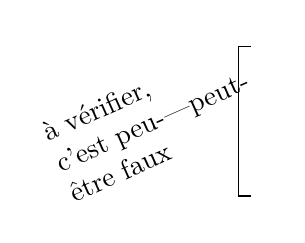
\begin{tikzpicture}
\draw (2.1,0) -- (1.95,0) -- (1.95,1.9) -- (2.1,1.9);
\node[align=left,rotate=24] at (0.85,0.95) {à vérifier,\\c'est \unsure{peu-|peut-}\\\uline{être faux}};
\end{tikzpicture}}}

2.7. Arrivé à ce point de mes brillantes conjectures, je m'aperçois avec consternation qu'elles sont fausses telles quelles, malgré les indications concordantes militant en leur faveur. De façon précise, soit $k$ un corps de caractéristique \deleted{nulle} $p>0$. Je dis qu'\uline{il n'est pas possible}, \uline{pour tout} $k$-\uline{schéma} $S$ \uline{de type fini}, \uline{de dimension} $\le\deleted{1}\inserted{0}$, \uline{avec} $S_{\text{rég}}$ \uline{régulier}, \uline{et tout schéma elliptique} \uline{$A$ sur} $S$, \uline{de mettre sur} $H^1_{\operatorname{DR}}(A/S)$ \uline{une stratification relativement à} $k$, \uline{qui soit fonctorielle en} $A$ \uline{et compatible avec les changements de base}. L'ennui, comme d'habitude, provient des courbes elliptiques de Hasse nul. Appliquant en effet les deux fonctorialités postulées, on trouve que l'homomorphisme ``frobenius'' qui va de $M^{(p)}$ dans $M$ ($M=H^1_{\operatorname{DR}}(A/S)$) serait compatible avec la stratification. Si alors $s\in S$ est un point correspondant à un $A_s$ de Hasse nul, i.e. tel que frobenius sur $H^1_{\operatorname{DR}}(A_s)$ soit de carré nul, on en conclurait aisément, grimpant sur les voisinages infinitésimaux de $s$, que la même propriété serait vraie aux points voisins de $s$, ce qui est évidemment faux p.ex. pour la famille modulaire.
\margin{\figure{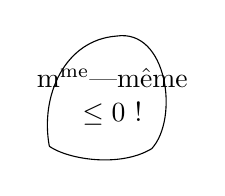
\begin{tikzpicture}
\draw (0,0.15) .. controls (-0.12,0.8) and (0.2,1.5) .. (0.85,1.55) .. controls (1.5,1.65) and (1.65,0.5) .. (1.3,0.12) .. controls (0.9,-0.12) and (0.25,-0.02) .. (0,0.15);
\node[align=center] at (0.8,0.78) {\unsure{m\textsuperscript{me}|même}\\$\le0$ !};
\end{tikzpicture}}}
\margin{26}


\scanpage{28}
\mspage{26}
Ceci montre que décidément, il faut en rabattre, et que dans le titre du Chapitre et les considérations de 2.2., c'est à condition de prendre partout des isocristaux qu'il reste une chance d'une théorie du genre de celle envisagée précédemment. Il est fort possible d'ailleurs que la notion de isocristal que j'ai adoptée est encore trop restrictive, en ce sens que dans la description de 1.13. il faudra peut-être prendre des stratifications en caractéristique nulle qui ne se prolongeraient pas nécessairement sur le schéma formel sur $W$ = vecteurs de Witt tout entier. C'est une analyse soigneuse du calcul-clef de Washnitzer-Monsky qui devrait permettre de tirer cette question au clair.
\margin{\figure{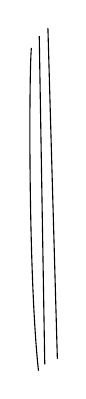
\begin{tikzpicture}
\draw (0,0) .. controls (-0.13,1.2) and (-0.12,3.8) .. (-0.09,4.1);
\draw (0.08,0.08) -- (0.01,4.25);
\draw (0.24,0.15) -- (0.12,4.35);
\end{tikzpicture}}}

2.8. Il se pose la question, d'autre part, pour quels schémas abéliens les énoncés 1º et 3º de 2.4, 2.5. et 2.6. sont valables, en dehors du cas déjà signalé: $S$ de caractéristique nulle.
\figure{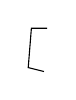
\begin{tikzpicture}\draw (0.2,0.55) -- (0,0.55) -- (-0.04,0.05) -- (0.16,0);\end{tikzpicture}}
\deleted{J'aurais assez tendance à croire que si $A$ est une VA définie sur un corps $k$ de car.$p>0$, alors ce qu'on veut (savoir l'indépendance de $G(B)$ d'un relèvement infinitésimal choisi $B$ de $A$) est vrai, pour tout anneau artinien de corps résiduel $k$, \uline{si et seulement si} $A$ est ``ordinaire'' i.e. a sur la clôture algébrique de $k$ le nombre maximum de points d'ordre $p$. Notes qu'il n'est pas nécessaire de supposer $k$ parfait (la question est manifestement géométrique), donc le groupe \deleted{formel} \inserted{p-divisible} de $A$ sur $k$ ne se décompose pas nécessairement en produit d'un étale par un infinitésimal. On aurait alors, pour de telles VA au moins, la description très explicite des relèvements infinitésimaux en termes du relèvement d'une filtration d'un module à la Dieudonné. Cette conjecture semble raisonnable car on a fait ce qu'il fallait pour éliminer des ennuis comme dans l'exemple de 2.7., d'autre part cela s'harmonise fort bien avec le tapis Serre des relèvements canoniques \inserted{et des modules} de variétés abéliennes du type ``ordinaire''.

Il serait évidemment tentant d'espérer qu'un énoncé du même type serait vrai pour une base quelconque, pourvu que toutes les fibres de $A/S$ soient des VA ordinaires. Mais cela est certainement faux avec cette généralité, même pour des schémas elliptiques, essentiellement toujours pour les même rai-\inserted{sons.}}
\margin{Faux, \unsure{ce} n'est \uline{jamais} vrai en car $p>0$ !}
\margin{\figure{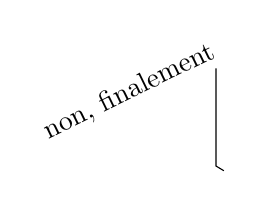
\begin{tikzpicture}
\draw (2.25,0) -- (2.15,0.06) -- (2.15,1.3);
\node[rotate=26] at (1.05,1.0) {non, \unsure{finalement}};
\end{tikzpicture}}}
\margin{27}


\scanpage{29}
\mspage{27}
\deleted{Pren\deleted{\unsure{n}}ons en effet un schéma \inserted{$S$} modulaire à échelons \deleted{$S$} pour variations de courbes elliptiques, et localisons en $\underline{Z}_p$, soit encore $S$ le schéma lisse sur $\underline{Z}_p$ obtenu. On a sur $S$ le Module loc libre de rang 2 $H^1_{\operatorname{DR}}(A/S)$, et quand on enlève de $S$ le nombre fini de points fermés correspondants à Hasse nul, on aurait une stratification \deleted{absolue sur} rel. à $\underline{Z}_p$ sur ce Module. Pour des raisons de pureté évidentes, celle-ci se prolongerait au dessus de $S$ tout entier, d'où une stratification sur le $H^1_{\operatorname{DR}}$ de la famille modulaire de courbes elliptiques, en caractéristique $p$. Celle-ci serait alors compatible avec frobenius (car elle l'est dans le complémentaire de l'ensemble fini des points de Hasse nul), ce qui contredit nos réflexions de 2.7.}

Il n'est pas exclu entièrement, cependant, que en restant en car.$p>0$, l'énoncé sur la non-variation \deleted{\unsure{de $G(A)$}} infinitésimale de $G(A)$ avec $A$, $A$ partout ordinaire, soit vrai. Cela impliquerait que sur l'ouvert des valeurs ``ordinaires'' de l'invariant, le $H^1_{\operatorname{DR}}$ a une stratification canonique, mais celle-ci ne se prolongerait pas à la courbe modulaire toute entière. Mais je dois dire que ce drôle de comportement, où on aurait une stratification naturelle en car.$p$ et une autre en car. 0, sans qu'elles veuillent se recoller, semble assez canularesque.

\inserted{[}Les considérations précédentes font bien ressortir la nature ``infinie'' de la notion de stratification, par contraste avec celle de connexion, malgré les trompeuses apparences de la caractéristique nulle. Ainsi, sur le $H^1_{\operatorname{DR}}$ de la famille modulaire sur $\underline{Z}$ \deleted{\unsure{pade|par}} \inserted{de} schémas elliptiques, il y a \deleted{sur} \inserted{au dessus de} la fibre générique $S_{\underline{Q}}$ de $S$ une stratification naturelle, mais nous venons de voir (ou presque ...) que cette\deleted{b} stratification ne s'étend pas en une stratification sur $S_U$, $U$ un ouvert non vide de $\operatorname{Spec}(\underline{Z})$. (Le ``presque'' provient du fait qu'il n'est pas absolument clair si la stratification qu'on obtiendrait ainsi en car.$p$ serait respectée par frobenius; il faut absolument tirer au clair cet exemple particulier !). C'est en un sens assez moral, puisque pour nous la \inserted{module à} stratification doit jouer dans une large mesure le rôle d'un faisceau $\ell$-adique, dont il partage
\margin{28}


\scanpage{30}
\mspage{28}
également les propriétés de rigidité.\inserted{]}

Pour en revenir à l'alinéa précédent, concernant un schéma abélien ``ordinaire'' en car. $p>0$, s'il n'est pas exclu que le $H^1_{\operatorname{DR}}$ admette une stratification canonique fonctorielle, il me semble eependant exclu, malheureusement, que celle-ci provienne d'un cristal \deleted{sur $S$} de modules sur $S$, i.e. que ceci reste vrai en remplaçant $S$ par toute extension infinitésimale, pas néc de car.$p$, \inserted{(tout-au moins} en admettant que la connexion associée à la stratification en question soit la connexion de Gauss-Manin\inserted{)}. En effet, appliquant une telle hypothèse au schéma modulaire $S$ sur $\underline{Z}_p$ précédent, dont on enlèverait les points de Hasse nul d'abord\inserted{, d'où $S'$}, on conclurait sauf erreur que \deleted{sur $S$ tout entier,} la stratification qu'on a en caractéristique nulle sur $H^1_{\operatorname{DR}}$ se prolongerait à $S$ tout entier, car elle se \inserted{``}recollerait'' en un sens évident avec la \deleted{connexion} stratification qu'on aurait \deleted{sur le} \inserted{au dessus du} complété p-adique de $S'$ (ce qui doit impliquer le prolongement sur $S$ de façon assez formelle). Mais alors on aurait en car.$p$ une stratification du $H^1_{\operatorname{DR}}$ au dessus du schéma modulaire tout entier, Hasse nul inclus, ce qui est absurde comme on l'a déjà remarqué. Il faut en conclure, hélas, que si les isocristaux, et le cas échéant les modules stratifiés même en caractéristique \deleted{nulle} $p>0$, ont des chances d'être des outils convenables pour l'étude de familles de variétés abéliennes, celle de cristal elle-même semble irrémédiablement trop fine, même en se restreignant à des familles de VA ``ordinaires'' en car $p>0$. Elle peut tout au mieux \unsure{de|se} prêter au cas d'un schéma de base réduit à un point, spectre d'un corps pas nécessairement parfait, et on peut alors espérer les résultats les plus satisfaisants en se bornant aux VA ordinaires? - Pour que la notion de cristal elle-même puisse être utilisée pour des schémas abéliens sur des bases plus générales, il semble donc qu'il faille imposer aux familles envisagées des restrictions très sérieuses, consistant à imposer la variation infinitésimale du $G(A)$. Cela semble assez proche du point de vue de Serre, qui étudie les variations de VA (éventuellement à multiplication complexe donnée) en imposant à priori l'espace tangent (et l'action de la MC dessus) ...
\margin{29}


\scanpage{31}
\mspage{29}
\uline{Chapitre} 3\deleted{\unsure{2|4}} \uline{Remarques sur les groupes} p-\uline{divisibles}.

3.1. Bien sûr, en même temps que pour les VA, je dois en rabattre sur les groupes formels. Je veux simplement signaler que la construction de $G(A)$ dans 2.6. doit pouvoir se paraphraser sans difficulté pour un groupe p-di\inserted{vi}sible $\phi$ sur un préschéma $S$ à caractéristiques résiduelles égales au même $p$. En effet les homomorphismes de ce groupe\deleted{s} dans le groupe formel associé à $\underline{G}_a$ sont triviales (en particulier, $\phi$ n'a pas d'automorphismes infinitésimaux). D'autre part (sauf erreur) le faisceau en \deleted{groupes} \inserted{modules} des $H^2$ de $\phi$ à valeurs dans le groupe formel \uline{a}ssocié à $\underline{G}_a$ (au sens du complexe du groupe $\phi$, variante formelle), est un Module localement libre de rang $g^*$, où $g^*$ est la dimension du groupe dual de $\phi$, soit $\phi^*$; plus précisément, ce Module doit être canoniquement isomorphe à $\underline{\operatorname{Lie}}(\phi^*)$\inserted{$=\underline{t}_{\phi^*}$}. \inserted{(}Tout ceci est suggéré par les résultats de Tate et Lubin sur les modules de groupes formels; je dois avouer d'ailleurs que je n'ai pas essayé de tirer au clair ce qu'il faut entendre, dans ce contexte, par ``le groupe formel associé à $\underline{G}_a$'', et s'il y a lieu de prendre le groupe formel purement infinitésimal.\inserted{)} Il s'impose alors de paraphraser la construction de Serre, en regardant l'extension \deleted{canonique} universelle de $\phi$ par un groupe formel vectoriel, qui sera ici le groupe formel (covariant) de $\underline{t}_{\phi^*}$. Désignant par $G(\phi)$ cette extension, son algèbre de Lie $H(\phi)$ sera une extension
\[
(*)\qquad 0\longrightarrow\underline{t}_{\phi^*}^{\vee}\longrightarrow\underline{H}(\phi)\longrightarrow\underline{t}_{\phi}\longrightarrow0.
\]
Bien entendu, $G(\phi)$ et par suite $\underline{H}(\phi)$ seront fonctoriels en $\phi$, et compatibles avec changement de base. Alors qu'il est certainement vrai, dans un sens qu'il conviendrait de préciser, que \deleted{\unsure{$\underline{H}(\phi)$}} $G(\phi)$ varie ``moins que $\phi$'', quand on fait varier $\phi$ infinitésimalement dans une famille, il n'est pas vrai pour autant que $G(\phi)$ soit indépendant de telles variations (à l'exception, probablement, de celles du premier ordre), i.e. puisse être considéré comme provenant d'un cristal en groupes \deleted{p-divisibles} \inserted{$\pm$ formels}. Cela sera le cas\deleted{,} seulement, sans doute, quand $\phi$ sera extension d'un groupe \deleted{\unsure{formel}} ind-étale par un groupe p-divisible torique, \inserted{et $S$ réduit à un point (?).} Dans le cas général, il semble intéressant d'étudier les variations
\margin{30}


\scanpage{32}
\mspage{30}
infinitésimales de $\phi$, quand on se fixe celles de $G(\phi)$ à l'aide d'un cristal en groupes $\underline{G}$.

3.2. En tous cas, l'extension $(*)$ semble un invariant intéressant du groupe p-divisible envisagé. Il subsiste, par passage à la limite, en passant \deleted{\unsure{du|à}} au cas où $S$ est \deleted{un schéma formel noethérien} par exemple le spectre d'un anneau $A$ noethérien j-adique séparé et complet, où $J$ est un idéal tel que $A/J$ soit à caractéristiques résiduelles égales à $p$. On trouve par exemple un bon invariant quand $A$ est un anneau de valuation discrète complet, éventuellement d'inégales caractéristiques, à caractéristique résiduelle $p$. Dans le cas où le groupe formel\deleted{,} réduit a la structure triviale \deleted{en} mentionnée plus haut dans 3.1., et que le corps résiduel $k$ est parfait, d'où un module de Dieudonné $M$ sur $W$ (de rang $g+g'$), il semble donc, d'après la remarque faite dans 3.1., que la donnée d'un relèvement du groupe p-divisible qu'on a sur $k$ en un groupe p-divisible sur $A$, soit entièrement équivalente à la donnée d'un relèvement de la filtration de $M\otimes_Wk$ donnée par $(*)$, en une filtration de type $(g,g^*)$ de $M\otimes_WA$, \deleted{Comme} Il serait bien intéressant d'essayer de déterminer, en termes d'une telle donnée, quel est le module de Tate correspondant à la fibre générique de $\phi$ ! On aimerait préciser également, pour des groupes p-divisibles plus généraux, quelle quantité d'information est liée à l'extension $(*)$\inserted{,} qui remplace ici le $H^1$ de De Rham.
\margin{31}


\scanpage{33}
\margin{Réduction des courbes elliptiques et $T_p(E)$}
\margin{(cf. aussi livre de Serre ``Abelian $l$-adic representations'')}
\margin{32}


\scanpage{34}
Courbes elliptiques sur un \deleted{anneau de} corps local à car. résiduelle $p>0$: étude infinitésimale.

$A$ anneau de val. discrète complet, corps des fractions $K$, corps résiduel $k$ de car $p>0$.

$E_K$ courbe elliptique sur $K$, \deleted{\unsure{d'où un grp Module|d'où un grp Modèle}}
\figure{\begin{tikzpicture}\draw[->] (0,0.3) -- (0,0);\end{tikzpicture}}

1º) \uline{$K$ de car 0} i.e. $T_p(E_{\overline{K}})_{\text{ét}}$ \uline{de rang 2} \deleted{\unsure{libre}}.
\margin{\unsure{[}et $T_p(E_{\overline{K}})_{\text{ét}}=T_p(E_{\overline{K}})$]}

On veut étudier les structures possibles pour ce module galoisien.

a) $E_K$ a ``bonne réduction'' i.e. $E$ provient d'un schéma elliptique $E$ sur $A$, \uline{et} $E_k$ est ``ordinaire''.

Alors $T_p(E_K)$ est \inserted{can.} extension d'un \deleted{module} \inserted{$L$} de rang 1, \inserted{\uline{m. n. ramifié}}, par un \deleted{autre} module de la forme
\[
\deleted{\operatorname{Hom}}\quad L^{\vee}\otimes T_p(G_m)=L^{\vee}[1].
\]
\margin{\diagram{\begin{tikzcd}[ampersand replacement=\&,column sep=large]
0\arrow[r]\&L^{\vee}(1)\arrow[r,phantom,"{\unsure{\text{---}|\longrightarrow}}" description]\&T_p(E_K)\arrow[r]\&L^{\unsure{*|\vee}}\arrow[r,phantom,"{\unsure{\text{---}|\longrightarrow}}" description]\&\unsure{\cdot|0}
\end{tikzcd}}}
De plus, l'extension, \deleted{qui} est donnée par un élément de
\[
H^1(K,\deleted{\unsure{L^{\vee}\otimes L^{\vee}|\operatorname{Hom}(L,L^{\vee})}}L^{-2}\otimes_{Z_p}T_p(G_m)),
\]
qui dans le cas où $A$ est à corps résiduel sép. clos (donc $L$ trivial sur $A$) s'identifie à
\[
H^1(K,T_p(G_m))\otimes_{Z_p}L_0^{-2}
\simeq\left(\varprojlim\unsure{K^*/\deleted{\unsure{Z|\otimes}}{\inserted{K^*}}^{p^n}|K^*\otimes Z/p^n}\right)\otimes_{Z_p}L_0^{-2}
\simeq\operatorname{Hom}(L_0^2,\widehat{K^*}).
\]
\margin{$L_0$: valeur en $k$}

\margin{33}


\scanpage{35}
\unsure{Et|A} cet \deleted{extension provient en fait} élément est en fait ``bien ramifié'' i.e. est dans le sous-groupe
\[
\operatorname{Hom}_{Z_p}(L^2,\underbrace{A^{**}}_{\text{\unsure{Eins-einheiten|1-unités}}})\simeq L^{-2}\otimes_{Z_p}A^{**}.
\]

[\uline{NB.} \unsure{Ça fait donc qu'on a un invariant|On voit donc qu'on a un invariant} à déterminer \uline{mod \deleted{multiplication} \inserted{exponentiation} par un carré de \deleted{\unsure{un|u}} \inserted{unités} $p$-adiques} \dots]

\margin{N.B. L'extension $T_p(E_{\unsure{K|\overline K}})$ peut être triviale (relèvements de Serre) ou non. Cas intéressant: \unsure{si|s'il} est d'ordre fini \dots}
\margin{En tous cas, \unsure{on aura|on a} une opération \uline{abélienne} [dans le cas \unsure{gén.|précédent}]}

b) $E_K$ a bonne réduction, et $E_k$ est ``hypersingulière'' i.e. est non ordinaire. J'ai envie de conjecturer que alors la représentation de $\pi_1(K)$ dans $T_p(E_{\overline K})$ est $\unsure{\frac12|Q}$-simple, voire que l'image de $\pi_1(K)$ dans $\operatorname{Aut}(T_p(E_{\overline K}))$ est un sous-groupe ouvert \dots ??
\margin{\figure{\begin{tikzpicture}\draw (0.7,3) .. controls (0.2,1.5) and (0.2,0.6) .. (0.9,0);\node at (0,1.4) {?};\end{tikzpicture}}}

$(a'+b')$ $E_K$ n'a pas \inserted{\unsure{néc.|néc?}} bonne réduction, mais l'invariant de $E$ est entier, i.e. après extension finie de $K$, on obtient bonne réduction. Ceci splitte en deux cas, a') réduction ordinaire après ext. de la base $K$, i.e. quand on a un invariant ordinaire. Alors l'opération de $\unsure{\pi^1(K)|\pi_1(K)}$ est ``métabélienne''. b') quand on est hypersingulier. Mais \deleted{\unsure{cq|que}} si la conjecture dans b) est valable, les conclusions de cette conjecture valent aussi dans le cas b').
\margin{NB.}
\margin{34}


\scanpage{36}
que cet élément a une image \uline{non nulle} dans $Z_p$, donc que l'extension ne provient pas d'une extension de groupes $p$-divisibles \uline{sur $A$}.

\uline{Question} Quel est l'élément obtenu de $Z_p$ ! est-ce tjrs un entier, voire un entier $>0$ ?

2º) \uline{Cas} $\operatorname{car}K\unsure{>|\ne}0$ \uline{donc} $\operatorname{car}K=p$

\deleted{\unsure{Cela|Ce cas}} Il y a lieu d'étudier $T_p(K)$, qui ne s'explicite plus en général exclusivement en termes de modules galoisiens.

A) Cas $j$ entier (bonne réduction). a) \unsure{Si|si} quand on est ordinaire, alors $E_K$ est ordinaire, donc
\figure{\begin{tikzpicture}\fill (0,0) circle (0.025);\draw[line width=0.6pt] (0.07,0)--(1.2,0);\fill (0.27,0) ellipse (0.08 and 0.025);\fill (1.2,0) ellipse (0.05 and 0.025);\end{tikzpicture}}
$T_p(E_K)$ est une extension d'un $L_K$ par $L_K^{\vee}\otimes T_p(G_m)$, et l'extension est donnée par un invariant dans $L^{-2}\otimes A^{**}$ (pas \unsure{nulle|nul} dans $L^{-2}\otimes$
\margin{(\unsure{si|qui} $k$ alg. clos)}
\figure{\begin{tikzpicture}\draw[->] (0,-0.35) .. controls (-0.1,0.1) and (0.2,0.15) .. (1.5,0.3) -- (4.3,0.65);\end{tikzpicture}}
\margin{35}


\scanpage{37}
\uline{NB} Si l'invariant $j$ est entier, alors on peut conjecturer que \deleted{la réduction de} $E_K$ a bonne réduction ssi il en est de $\unsure{\overline{\mathrm m}|=}$ $T_p(E_K)$, le grp $p$-divisible associé.
\margin{?}

c) L'invariant $j$ n'est pas entier.

Alors le \uline{modèle de \uline{Néron}} \inserted{$\unsure{\overline E|E}$} est tel que $E_k^0$ est une \inserted{forme de} $G_m$. Par suite, on conclut que dans ${}_{p^{\unsure{\nu|n}}}\unsure{\overline E|E}$ il y a un sous-groupe canonique \deleted{fini de} forme de $\mu_{p^{\unsure{\nu|n}}}$.
\margin{[qui n'est pas fini sur $A$ en gén]}
\figure{\begin{tikzpicture}\draw (0,-0.35) .. controls (0.15,0.2) and (0.15,0.2) .. (0.7,0.25)--(5,0.25) .. controls (5.3,0.25) and (5.4,0.3) .. (5.45,0.35);\end{tikzpicture}}

On trouve ainsi dans $T_p(E_K)$ un sous-groupe, qui est une forme \uuline{finiment} tordue de $T_p(G_m)$.
\margin{[donc un $T_p(G_m)$ défini au signe près]}
\figure{\begin{tikzpicture}\draw (0,-0.3) .. controls (0.1,0.2) and (0.2,0.2) .. (0.6,0.25) -- (4.5,0.4) .. controls (4.8,0.45) and (5,0.4) .. (5.2,0.25);\end{tikzpicture}}

Donc si $k$ est sép. clos, on trouve que $T_p(E_K)$ admet un sous-module isomorphe (de façon \uline{canonique} mod signe] à $T_p(G_m)\inserted{{}=Z_p(1)}$, quotient étant nécessairement isomorphe à $Z_p$ [car $\det T_p(E_K)\simeq Z_p(1)$].
\figure{\begin{tikzpicture}\draw[->] (0,-0.3) .. controls (0.15,0.2) and (0.8,0.1) .. (1.2,0.55);\end{tikzpicture}}

L'extension est ici déterminée par un élément canonique de $\widehat{K^*}$ ext. de $Z_p$ [\unsure{provenant|provient} de $K^*/A^*$] par $A^{**}$. Je conjecture
\margin{36}

